% aistats version
\documentclass[twoside]{article}

\usepackage[accepted]{aistats2026}
% Packages copied from main.tex preamble
\usepackage[utf8]{inputenc}
\usepackage[T1]{fontenc}
\usepackage{url}
\usepackage{microtype}
\usepackage{textcomp}
\usepackage{lmodern}
\usepackage[english]{babel}
\usepackage{lipsum}
\usepackage{graphicx}
\usepackage{adjustbox}
\usepackage{scalerel,stackengine,amsmath}
\usepackage{subcaption}
\captionsetup[figure]{skip=-12pt}
\usepackage{tikz}
\usetikzlibrary{positioning, calc}
\usepackage{datetime}
\usepackage[ruled,linesnumbered]{algorithm2e}
\SetKwComment{Comment}{$\triangleright$ }{}
\RestyleAlgo{ruled}
\usepackage{accents}
\usepackage{xcolor,color}
\usepackage{parskip}
\usepackage{amssymb,amsmath,amsthm,amsfonts,mathtools, mathrsfs,bbold}
\usepackage[colorlinks=true, urlcolor=blue, linktoc=all]{hyperref}
\usepackage{thmtools}
\usepackage{stmaryrd}
\usepackage{multirow}
\usepackage{booktabs}
\usepackage{alphabeta}
\usepackage{thm-restate}
\usepackage{nicefrac}
\usepackage[capitalise,nameinlink,noabbrev]{cleveref}

% Commands and definitions copied from main.tex preamble
\newcommand*\circledaux[1]{\tikz[baseline=(char.base)]{\node[shape=circle,draw,inner sep=0.8pt] (char) {#1};}}
\NewDocumentCommand{\circled}{ m o }{\IfNoValueTF{#2}{ \circledaux{#1} }{ \stackrel{\circledaux{#1}}{#2} }}
\newcommand{\R}{\mathbb{R}}
\newcommand{\ones}{\mathbb{1}}

\makeatletter
\def\Hy@raisedlink@left#1{%
    \ifvmode
        #1%
    \else
        \Hy@SaveSpaceFactor
        \llap{\smash{%
        \begingroup
            \let\HyperRaiseLinkLength\@tempdima
            \setlength\HyperRaiseLinkLength\HyperRaiseLinkDefault
            \HyperRaiseLinkHook
        \expandafter\endgroup
        \expandafter\raise\the\HyperRaiseLinkLength\hbox{%
            \Hy@RestoreSpaceFactor
            #1%
            \Hy@SaveSpaceFactor
        }%
        }}%
        \Hy@RestoreSpaceFactor
        \penalty\@M\hskip\z@ 
    \fi
}
\makeatother

\newcommand\linktoproof[1]{{\normalfont[{\hyperlink{proof:#1}{$\downarrow$}}]}}
\newcommand\linkofproof[1]{\textbf{of \cref{#1}. }\newtarget{proof:#1}}

\newcommand{\bigomega}[1]{\Omega( #1 )}
\newcommand{\bigomegal}[1]{\Omega\left( #1 \right)}
\newcommand{\bigo}[1]{O( #1 )}
\newcommand{\bigol}[1]{O\left( #1 \right)}

\newcommand{\jmlrBlackBox}{\rule{1.5ex}{1.5ex}}
\providecommand{\BlackBox}{\jmlrBlackBox}
\newcommand{\jmlrQED}{\hfill\jmlrBlackBox\par\bigskip}
\providecommand{\proofname}{Proof}
\renewenvironment{proof}{\par\noindent{\bfseries\upshape \proofname\ }}{\jmlrQED}

\crefname{equation}{Eq.}{Eqs.}
\newcommand{\mP}{\mathcal{P}}
\newcommand{\mQ}{\mathcal{Q}}
\newcommand{\mA}{\mathcal{A}}
\newcommand{\mF}{\mathcal{F}}
\newcommand{\mX}{\mathcal{X}}
\newcommand{\verts}[1]{\mathcal{V}_{#1}}
\newcommand{\conv}[1]{\mathsf{conv}\left(#1\right)}
\newcommand{\aff}[1]{\mathsf{aff}\left(#1\right)}
\newcommand{\faces}[1]{{\mathsf{faces}^\ast}\left(#1\right)}
\newcommand{\facets}[1]{\mathsf{facets}\left(#1\right)}
\newcommand{\dist}[1]{\mathsf{dist}\left(#1\right)}
\newcommand{\proj}{\mathsf{Proj}}
\NewDocumentCommand{\pw}{o m}{\mathop{\delta\IfValueT{#1}{^{#1}}_{#2}}}
\NewDocumentCommand{\vf}{o m}{\mathsf{vf}\IfValueT{#1}{^{#1}}_{#2}}
\NewDocumentCommand{\diam}{o m}{D\IfValueT{#1}{^{#1}}_{#2}}
\newcommand{\innp}[1]{\left\langle #1 \right\rangle}
\newcommand\allbf[1]{{\textbf{#1}}}

\DeclareMathOperator*{\argmin}{\mathrm{arg\,min}}
\DeclareMathOperator*{\argmax}{\mathrm{arg\,max}}
\DeclarePairedDelimiter\ceil{\lceil}{\rceil}
\DeclarePairedDelimiter\floor{\lfloor}{\rfloor}
\newcommand{\norm}[1]{\| #1 \|}
\newcommand{\defi}{\stackrel{\mathrm{\scriptscriptstyle def}}{=}}
\newcommand{\defiin}{\stackrel{\mathrm{\scriptscriptstyle def}}{\in}}

\newtheorem{theorem}{Theorem}[section]
\newtheorem{lemma}[theorem]{Lemma}
\newtheorem{remark}[theorem]{Remark}
\newtheorem{proposition}[theorem]{Proposition}
\newtheorem{definition}[theorem]{Definition}
\newtheorem{corollary}[theorem]{Corollary}
\newtheorem{fact}[theorem]{Fact}
\newtheorem{example}[theorem]{Example}
\newtheorem{assumption}[theorem]{Assumption}

\hypersetup{colorlinks=true, linkcolor=blue, filecolor=magenta, urlcolor=blue, citecolor=blue}

\let\epsilon\varepsilon
% style=authoryear
%\usepackage[natbib, maxcitenames=3, maxbibnames=99, style=authoryear, hyperref, backref, useprefix=true, uniquename=false, doi=false,url=false,eprint=false]{biblatex} % useprefix is for `van', `von' etc. ;

\usepackage[
    natbib,
    backend=biber,
    maxcitenames=3,
    minalphanames=3,
    maxbibnames=99,
    style=authoryear,%alphabetic,
    hyperref,
    backref,
    useprefix=true,
    uniquename=false,
    doi=false,
    url=false,
    eprint=false
]{biblatex} % useprefix is for `van', `von' etc. ;








\usepackage{csquotes}               % Strongly recommended for biblatex
%\nocite{*}
\bibliography{refs}        %use a bibtex bibliography file refs.bib
%\bibliography{biblio_giommazz}   

%\bibliographystyle{plainnat}  %use the plain bibliography style

% ==== Add links to author names when citing
%\DeclareCiteCommand{\cite}
%  {\usebibmacro{prenote}}
%  {\usebibmacro{citeindex}%
%   \printtext[bibhyperref]{\usebibmacro{cite}}}
%  {\multicitedelim}
%  {\usebibmacro{postnote}}
%
%\DeclareCiteCommand*{\cite}
%  {\usebibmacro{prenote}}
%  {\usebibmacro{citeindex}%
%   \printtext[bibhyperref]{\usebibmacro{citeyear}}}
%  {\multicitedelim}
%  {\usebibmacro{postnote}}
%
%\DeclareCiteCommand{\parencite}[\mkbibparens]
%  {\usebibmacro{prenote}}
%  {\usebibmacro{citeindex}%
%    \printtext[bibhyperref]{\usebibmacro{cite}}}
%  {\multicitedelim}
%  {\usebibmacro{postnote}}
%
%\DeclareCiteCommand*{\parencite}[\mkbibparens]
%  {\usebibmacro{prenote}}
%  {\usebibmacro{citeindex}%
%    \printtext[bibhyperref]{\usebibmacro{citeyear}}}
%  {\multicitedelim}
%  {\usebibmacro{postnote}}
%
%\DeclareCiteCommand{\citeauthor}
%  {\usebibmacro{prenote}}
%  {\ifciteindex
%     {\indexnames{labelname}}
%     {}%
%   \printtext[bibhyperref]{\printnames{labelname}}}
%  {\multicitedelim}
%  {\usebibmacro{postnote}}
%
%\DeclareCiteCommand{\footcite}[\mkbibfootnote]
%  {\usebibmacro{prenote}}
%  {\usebibmacro{citeindex}%
%  \printtext[bibhyperref]{ \usebibmacro{cite}}}
%  {\multicitedelim}
%  {\usebibmacro{postnote}}
%
%\DeclareCiteCommand{\footcitetext}[\mkbibfootnotetext]
%  {\usebibmacro{prenote}}
%  {\usebibmacro{citeindex}%
%   \printtext[bibhyperref]{\usebibmacro{cite}}}
%  {\multicitedelim}
%  {\usebibmacro{postnote}}
%
%\DeclareCiteCommand{\textcite}
%  {\boolfalse{cbx:parens}}
%  {\usebibmacro{citeindex}%
%   \printtext[bibhyperref]{\usebibmacro{textcite}}}
%  {\ifbool{cbx:parens}
%     {\bibcloseparen\global\boolfalse{cbx:parens}}
%     {}%
%   \multicitedelim}
%  {\usebibmacro{textcite:postnote}}
%=========================

% ==== Add links to the titles of citing papers, instead of having the text with the URL there
% add these options to biblatex [doi=false,url=false]{biblatex}
% to disable other links. We also need colorlinks with hyperref

\newbibmacro{string+doiurlisbn}[1]{%
  \iffieldundef{doi}{%
    \iffieldundef{url}{%
      \iffieldundef{isbn}{%
        \iffieldundef{issn}{%
          #1%
        }{%
          \href{http://books.google.com/books?vid=ISSN\thefield{issn}}{#1}%
        }%
      }{%
        \href{http://books.google.com/books?vid=ISBN\thefield{isbn}}{#1}%
      }%
    }{%
      \href{\thefield{url}}{#1}%
    }%
  }{%
    \href{https://doi.org/\thefield{doi}}{#1}%
  }%
}

\DeclareFieldFormat{title}{\usebibmacro{string+doiurlisbn}{\mkbibemph{#1}}}
\DeclareFieldFormat[article,incollection,inproceedings]{title}%
    {\usebibmacro{string+doiurlisbn}{#1}}
    %{\usebibmacro{string+doiurlisbn}{\mkbibquote{#1}}}
\usepackage{todonotes}
\newif\ifTODO 

% \TODOtrue
%\ifanonsubmission \TODOfalse \fi
\TODOfalse

\definecolor{aquamarine}{rgb}{0.5, 1.0, 0.83}

\newcommand{\Dav}[1]{\ifTODO \todo[inline,author=DM, caption={}, color=yellow]{#1} \fi}
\newcommand{\Pac}[1]{\ifTODO \todo[inline,author=PC, caption={}, color=magenta]{#1} \fi}
\newcommand{\Eli}[1]{\ifTODO \todo[inline,author=EW, caption={}, color=magenta]{#1} \fi}
\newcommand{\Gab}[1]{\ifTODO \todo[inline,author=GI, caption={}, color=aquamarine]{#1} \fi}
\newcommand{\Seb}[1]{\ifTODO \todo[inline,author=SP, caption={}, color=green]{#1} \fi}

\newcommand{\dav}[1]{\ifTODO \todo[size=\scriptsize, color=yellow]{DM: #1}{} \fi}
\newcommand{\pac}[1]{\ifTODO \todo[size=\scriptsize, color=magenta]{PC: #1}{} \fi}
\newcommand{\eli}[1]{\ifTODO \todo[size=\scriptsize, color=magenta]{EW: #1}{} \fi}
\newcommand{\gab}[1]{\ifTODO \todo[size=\scriptsize, color=aquamarine]{GI: #1}{} \fi}
\newcommand{\seb}[1]{\ifTODO \todo[size=\scriptsize, color=green]{SP: #1}{} \fi}

\newcommand{\gabrev}[1]{\textcolor{black}{#1}}
\newcommand{\gabrebuttal}[1]{\textcolor{red}{#1}}

\ifTODO
% Make the paper wider if ifTODO is set so that the notes fit
\paperwidth=\dimexpr \paperwidth + 6cm\relax
\oddsidemargin=\dimexpr\oddsidemargin + 3cm\relax
\evensidemargin=\dimexpr\evensidemargin + 3cm\relax
\marginparwidth=\dimexpr \marginparwidth + 3cm\relax
\fi

\usepackage{xparse}
\usepackage{xargs} % define commands with multiple arguments with default a value http://www.texfaq.org/FAQ-twooptarg

\newcommand\newlink[2]{\hyperlink{#1}{\normalcolor #2}}
\makeatletter
\newcommand\newtarget[2]{\Hy@raisedlink{\hypertarget{#1}{}}#2}
\makeatother


\newcommand{\PL}{\newlink{def:acronym_polyak_lojasiewicz}{PL}}
\newcommand{\QG}{\newlink{def:acronym_quadratic_growth}{QG}}
\newcommand{\FW}{\newlink{def:acronym_frank_wolfe}{FW}}
\newcommand{\AFW}{\newlink{def:acronym_away_frank_wolfe}{AFW}}
\newcommand{\LMO}{\newlink{def:acronym_linear_minimization_oracle}{LMO}}



\newcommand{\w}[1]{\operatorname{\delta}_{#1}}
\newcommand{\what}{\operatorname{\bar{\delta}}}
\newcommand{\X}{\mathcal{X}}

\newcommand{\wface}[2]{\operatorname{\Delta}_{#1}(#2)}
\newcommand{\whatface}[2]{\operatorname{\bar{\Delta}}_{#1}(#2)}


%% Config caption names:
%\renewcommand{\lstlistingname}{Algorithm}

% Wrapper for pseudocode
\usepackage{algorithm}
%\usepackage{algpseudocode}
\usepackage{algcompatible}
\algnewcommand{\lst}{\texttt{lst}}
\algnewcommand{\slst}{\texttt{slst}}
\algnewcommand{\SEND}{\textbf{send}}

\newsavebox{\algleft}
\newsavebox{\algright}

\renewcommand{\algorithmiccomment}[1]{\hfill  $\diamond$ #1}

\renewcommand{\algorithmicrequire}{\textbf{Input:}}
\renewcommand{\algorithmicensure}{\textbf{Output:}}

\makeatletter
\newcounter{algorithmicH}% New algorithmic-like hyperref counter
\let\oldalgorithmic\algorithmic
\renewcommand{\algorithmic}{%
  \stepcounter{algorithmicH}% Step counter
  \oldalgorithmic}% Do what was always done with algorithmic environment
\renewcommand{\theHALG@line}{ALG@line.\thealgorithmicH.\arabic{ALG@line}}
\makeatother


% ========================================================
\makeatletter
\newenvironment{breakablealgorithm}
  {% \begin{breakablealgorithm}
   \begin{center}
     \refstepcounter{algorithm}% New algorithm
     \hrule height.8pt depth0pt \kern2pt% \@fs@pre for \@fs@ruled
     \renewcommand{\caption}[2][\relax]{% Make a new \caption
       {\raggedright\textbf{\ALG@name~\thealgorithm} ##2\par}%
       \ifx\relax##1\relax % #1 is \relax
         \addcontentsline{loa}{algorithm}{\protect\numberline{\thealgorithm}##2}%
       \else % #1 is not \relax
         \addcontentsline{loa}{algorithm}{\protect\numberline{\thealgorithm}##1}%
       \fi
       \kern2pt\hrule\kern2pt
     }
  }{% \end{breakablealgorithm}
     \kern2pt\hrule\relax% \@fs@post for \@fs@ruled
   \end{center}
  }

%\newcommand{\theHalgorithm@line}{\thealgorithm.\arabic{algorithm@line}}

\makeatother


% If your paper is accepted, change the options for the package
% aistats2026 as follows:
%
%\usepackage[accepted]{aistats2026}
%
% This option will print headings for the title of your paper and
% headings for the authors names, plus a copyright note at the end of
% the first column of the first page.

% We also include a `preprint' option for non-anonymous preprints. 
% Change the options for the package aistats2026 as follows:
%
%\usepackage[preprint]{aistats2026}
%
% This option will print headings for the title of your paper and
% headings for the authors names, but does not print the copyright and 
% venue note at the end of the first column of the first page.

% If you set papersize explicitly, activate the following three lines:
%\special{papersize = 8.5in, 11in}
%\setlength{\pdfpageheight}{11in}
%\setlength{\pdfpagewidth}{8.5in}

% If you use the natbib package, activate the following three lines:
%\usepackage[round]{natbib}
%\renewcommand{\bibname}{References}
%\renewcommand{\bibsection}{\subsubsection*{\bibname}}

% If you use BibTeX in apalike style, activate the following line:
%\bibliographystyle{apalike}

\begin{document}

% If your paper is accepted and the title of your paper is very long,
% the style will print as headings an error message. Use the following
% command to supply a shorter title of your paper so that it can be
% used as headings.
%
%\runningtitle{I use this title instead because the last one was very long}

% If your paper is accepted and the number of authors is large, the
% style will print as headings an error message. Use the following
% command to supply a shorter version of the author names so that
% they can be used as headings (for example, use only the surnames)
%
%\runningauthor{Surname 1, Surname 2, Surname 3, ...., Surname n}

\twocolumn[

\aistatstitle{Linear Convergence of the Frank-Wolfe Algorithm over Product Polytopes}

% \aistatsauthor{
% Gabriele Iommazzo \And
% David Mart\'inez-Rubio \And
% Francisco Criado \AND
% Elias Wirth \And
% Sebastian Pokutta
% }

% \aistatsaddress{
% Zuse Institute Berlin\\
% %Berlin,
% Germany
% \And
% Signal Theory and Communications Department\\
% %Carlos III University
% UC3M\\
% %Madrid,
% Spain
% \And
% Departamento de Matem\'aticas\\
% CUNEF Universidad\\
% %Madrid,
% Spain
% \AND
% Berlin Institute of Technology\\
% %Berlin,
% Germany
% \And
% Technische Universit\"at Berlin\\
% and Zuse Institute Berlin\\
% %Berlin,
% Germany }

\aistatsauthor{
Gabriele Iommazzo$^{1}$ \And
David Mart\'inez-Rubio$^{2}$ \And
Francisco Criado$^{3}$ \AND
Elias Wirth$^{4}$ \And
Sebastian Pokutta$^{1,5}$
}

\aistatsaddress{
$^{1}$ Zuse Institute Berlin, Germany \quad
$^{2}$ Carlos III University, Madrid, Spain \quad
$^{3}$ CUNEF Universidad, Madrid, Spain\\
$^{4}$ Berlin Institute of Technology, Germany \quad
$^{5}$ Technische Universit\"at Berlin and Zuse Institute Berlin, Germany
}

]

\begin{abstract}
We study the linear convergence of Frank-Wolfe algorithms over product polytopes. We analyze two condition numbers for the product polytope, namely the \emph{pyramidal width} and the \emph{vertex-facet distance}, based on the condition numbers of individual polytope components. 
As a result, for convex objectives that are $\mu$-Polyak-\L{}ojasiewicz, we show linear convergence rates quantified in terms of the resulting condition numbers.
We apply our results to the problem of approximately finding a feasible point in a polytope intersection in high-dimensions, and demonstrate the practical efficiency of our algorithms through empirical results.
\end{abstract}



















%%%%%%%%%%%%%%%%%%%%%%%%%%%%%%%%%%%%%%%%%%%%%%%%%%%%%%%%%%%%
% ------------------------------

\eli{ Some thoughts:
1. Since the characterization of the product pyramidal width is our main contribution, this should be highlighted more. the proofs of linear convergence are tiny variations of existing works in \citep{LJ15, wirth2024fast, GH15}.
2. Whoever wrote the proofs of the linear convergence theorems should very precisely articulate what was changed from existing works. The audience either knows the other proofs, then they only want to know the tricky change or they dont. Then, they need to be pointed to the easier/more general proof in the literature.
3. Do we know why we cannot do this affine-invariantly? The proof should still be affine-invariant as the algorithm remains affine-invariant. see \citep{wirth2024fast}.

DM: agree with 1 and 2. About 3, the constants of smoothness and PL are characterized for the original setting, without any affine transformation, so in this case we can quantify convergence. Most likely an affine invariant statement can be said as well, for the resulting abstract quantities
}


% At each step, this scheme would: a) compute an \LMO{} to check approximate feasibility over the intersection of the polytope constraints and a halfspace corresponding to a level set of the objective function; b) treat the \LMO{} of each polytope in the intersection individually as a black-box operator.
% Specifically, consider computing the \LMO{} $\min_{x \in \mP}\langle c, x \rangle$ over a polytope $\mP$.
% $\mP$ can be any polytope, including one defined as the product of several polytopes with multiple constraints. 
% We examine hyperplanes $Q_i$ orthogonal to $c$ representing level sets of the linear objective function, and the corresponding halfspaces $\mQ_i$. 
% Our method optimizes the \LMO{} by recursively solving, for $i = 1, \dots, T$ an approximate feasibility problem over $\mP \cap \mQ_i$, employing BPFW updates over $\mP \cap \mQ_i$.
% Initially, $Q_1$ is scaled such that $\mQ_1$ fully includes $\mP$, and $Q_2$ such that $\mQ_2$ completely excludes $\mP$. 
% For $i > 2$, binary search is employed on $\mQ_i$ to find a feasible point in $\mP \cap \mQ_i$ that improves the objective $c$. 
%The recursion would require $O(\log(\|c\|_{\infty}/\epsilon))$ \LMO{} calls to return an $\epsilon$-approximate solution.


\section{Introduction}\label{s:intro}

Frank-Wolfe algorithms (\newtarget{def:acronym_frank_wolfe}{\FW{}}), also known as Conditional Gradient methods, are widely used first-order optimization algorithms. They are particularly suited for constrained convex problems $\min_{x\in\X} f(x)$, for a convex compact set $\X$, where linear minimization over $\X$ is used to keep the iterates feasible. The simplicity of this family of methods, along with its projection-free nature, make it especially appealing in large-scale settings, where projections can be costly. This is often the case when the feasible set is a polytope \citep{BCC+23}.

More concretely, \FW{} methods compute iterates as combinations of extreme points in the feasible set $\mX$ returned by a linear minimization oracle (\newtarget{def:acronym_linear_minimization_oracle}{\LMO{}}):
\begin{equation}
g \mapsto \argmin_{x \in \mX} \innp{g, x} \tag{LMO}
\label{eq:lmo}
\end{equation}
on $\mX$, where $g$ is some vector, usually the current gradient of the objective function or an approximation thereof.
After computing \eqref{eq:lmo}, the standard \FW{} method takes a step from the current iterate in the direction of the \LMO{} solution.
In many scenarios, \eqref{eq:lmo}
is a cheaper alternative to the quadratic optimization problem that projections consist of, cf. \citep{Jag13}, and can be computed even when $\mX$ is defined implicitly, such as a convex hull of a set of points.

The convergence behavior of \FW{} methods is strongly influenced by the geometry of the constraint set, that of the function, and the location of the unconstrained minimizer. While sublinear rates are typical in general convex and smooth settings, it is known that linear convergence can be achieved under additional assumptions, such as global optimizers being in the interior of $\X$ \citep{wolfe1970convergence,guelat1986some}, strong convexity of the feasible set along with all global optimizers being outside of it \citep{levitin1966constrained}, or strong convexity of $f$ for $\X$ being a polytope having some positive condition number. This last assumption holds for one of several different notions of conditioning that have been defined \citep{lacoste2013affine,GH15,LJ15,BS15,penya2016vonneumann,PR18}, % the penya2016vonneumann paper uses a conditioning called the relative width
among which there is the pyramidal width and the vertex-facet distance that we use in this paper, cf. \cref{s:conditioning_convergence}.

A few works extend the applicability of the algorithms to larger classes of functions such as the ones satisfying the Polyak-Łojasiewicz (\newtarget{def:acronym_polyak_lojasiewicz}{\PL{}}) condition, as opposed to strong convexity \citep{BS15,BCC+23}.
We quantify the implications of our condition number results in terms of linear convergence rates for our applications. 

Importantly, we note that much of the aforementioned theory remains confined to the setting of single polytopes, with limited understanding of how favorable properties like good condition numbers might extend and compose in more structured domains. In this work, we focus on optimization over \emph{product polytopes}.

This setting arises naturally in machine learning applications, specially via the feasibility problem for the intersection of several feasible sets, such as in image representation in computerized tomography \citep{CCC+09}, compressed sensing \citep{CCP12},
%It has also been studied in general for closed convex sets and it arises in a broad range of applications 
% Now the following are applications for the intersection of convex bodies that may not be polytopes
and including signal processing and statistical estimation \citep{SY98,CP10proximal}, image recovery \citep{Com96}, absolute value equations \citep{ACT23}, matrix completion \citep{RSV12} and robust PCA \citep{MA18}, SVMs \citep{LJS+13} and clustering \citep{BRZ23}.

A natural question is whether the good conditioning of individual polytopes can be lifted to the product domain in a way that still allows for linear convergence guarantees. We provide a surprising positive answer as the main contribution of this work: \emph{the product of well-conditioned polytopes inherits a form of good conditioning}, that enables linear convergence of \FW{} algorithms for smooth, convex, \PL{}-objectives by using either the pyramidal width or the vertex-facet distance.

Positive polytope condition numbers, such as the pyramidal width or the vertex-facet distance, typically capture how well the directions found by the \LMO{} in the polytope align with the idealized direction $x^\ast - x_t$ (from an iterate $x_t$ towards a minimizer $x^\ast$) relative to the direction of the gradient that was used for the \LMO{}, cf. \cref{a:linconv_pw}. Our findings imply that this alignment does not degrade much when considering a product polytope, with respect to the individual components.

We apply our results to the aforementioned important primitive in large-scale optimization: approximately finding a feasible point in the intersection of several polytopes or certifying that such intersection is empty. In other words, the problem of interest is, given $k \geq 2$ polytopes $\mP_i$,
\begin{equation}
\text{find } x \in \bigcap_{i=1}^k \mathcal{P}_i\,, \tag{P}
\label{prob:cfp}
\end{equation}
% closed convex sets in $\R^n$,
if it exists, or determine that the intersection is empty. An  \emph{$\epsilon$-approximate} solution of \eqref{prob:cfp} consists of finding a point whose Euclidean distance to the intersection is less than $\epsilon$, or determining that no such point exists. Finding an approximate feasible point in the intersection of $k$ polytopes can be turned into an approximate solver for linear programming over such intersection as feasible set, by performing a binary search objective value, see, e.g., \citep{DVZ22} and references therein.

For the above task, we consider the Away Frank-Wolfe (\newtarget{def:acronym_away_frank_wolfe}{\AFW{}}) algorithm \citep{GM86} (see \cref{algo:AFW} in \cref{a:algos}) over the Cartesian product, where we have a variable for each polytope and minimize an objective that penalizes each of the pairwise distances between the $k$ variables, cf. \eqref{prob:intersection_k}. Our objective is convex, smooth and satisfies the \PL{} inequality. Naturally, this approach uses the \LMO{} of the resulting product polytope, that is, the product of the corresponding  \LMO{} outputs for each polytope component, which can be computed in parallel.

Our technical contributions are the following.

\paragraph{Contributions} 
\begin{itemize}
    \item Regarding polytope condition numbers, we show that, if the \textit{pyramidal widths} of two polytopes $\mathcal{P}_1$ and $\mathcal{P}_2$ are $\delta_{\mathcal{P}_1}$ and $\delta_{\mathcal{P}_2}$, that of the product is exactly $\delta_{\mathcal{P}_1} \delta_{\mathcal{P}_2} /\sqrt{\delta_{\mathcal{P}_1}^2 + \delta_{\mathcal{P}_2}^2}$. This yields a pyramidal width $\delta_\mathcal{P} = \bigomega{\frac{1}{\sqrt{k}}\min_{i\in[k]} \delta_{\mathcal{P}_i}}$ for the product $\mathcal{P} = \prod_{i\in[k]} \mathcal{P}_i$ of $k$ polytopes.
    
    Our proof uses the \textit{affine pyramidal width}, which we introduce as a new equivalent characterization of the pyramidal width that is easier to work with in our proofs. Similarly, for the \textit{vertex-facet distance}, we show $\vf{\mP} = \min_{i\in[k]} \vf{\mP_{i}}$. 

   \item As a consequence of studying these two polytope condition numbers, we can quantify linear rates of convergence for the \AFW{} algorithm optimizing convex, smooth functions satisfying the \PL{} inequality over a product polytope, which inherits its conditioning from the components. 
   \item We apply our results to the problem of approximately finding a feasible point in the intersection of several polytopes, by minimizing \eqref{prob:intersection_k}, a convex, smooth and \PL{} objective.
   \item We substantiate our theoretical findings with empirical evidence, demonstrating the algorithm's applicability across large-scale optimization tasks.
\end{itemize}

The novel characterization of the pyramidal width as defined by the affine pyramidal width is of independent interest, and we believe that it can offer new insights into the optimization over polyhedral sets.


% ------------------------------
%%\section{Other Related Work} \label{s:literature}
%%\Dav{TODO, this still needs a lot of work. And there is too much content that is not so relevant }
%%
%% Some works study lower bounds for some of the polytope condition numbers condition numbers for several domains of interest \citep{wirth2023approximate, CFK23}. 
%%
%% BUT HEAVILY SUMMARIZE: To solve the convex feasibility problem \eqref{prob:cfp} for the intersection of closed, convex sets, most algorithms make use of projection operators onto the components $\mathcal{P}_i$, each consisting of a quadratic minimization problem. For $k=2$ sets, \eqref{prob:cfp} was initially tackled by von Neumann \citep{Von49} using an alternating projection algorithm, which was further studied by \citep{Gin18}.
%%Under favorable circumstances, e.g., intersecting a polytope and a hyperplane, this algorithm converges in finitely many steps.
%%However, this does not generally hold for two polytopes \citep[Example 5.2]{BBS21}.
%%Without additional assumptions, projection-based methods produce a solution 
%%% one such point 
%%%in $O(1/\epsilon^q)$ iterations with $q >0$ \citep{BS16,BC11,BPW23}, that is, 
%%with \emph{sublinear} rates \citep{BS16,BC11,BPW23}.
%%Linear rates have been achieved in several settings 
%%with additional conditions on the intersection \citep{GPR67}, on the distance between
%%an iterate and the intersection (proportional to the largest distance between that iterate and the sets) \citep{BB93,BB96,BT03}, on the alignment between the sets \citep{DIL15,BLM21}; see also \citep{BBS21}.
%%
%%%To this line of work belongs, for instance, the cyclic block-coordinate \FW{} algorithm \citep{BPS15},
%%%cycling through blocks one at a time.  An implementation of this algorithm adapted to solve the intersection problem for two compact, convex sets is presented in \citep{BPW23}.  These methods obtain sublinear convergence rates over product domains.  To the extent of our knowledge, the only exception is the block-coordinate \FW{} algorithm analyzed in \citep{BRZ23} for objectives satisfying the Kurdyka-Łojasiewicz property over product domains, which attains linear rates, although relying on a costly subroutine that limits its practical applicability.  Finally, \citep{GPL18} consider convex objectives over the product of compact convex sets, with one linear constraint linking the variables in the sets, that is relaxed within an augmented Lagrangian scheme. The resulting objective satisfies the \PL{} inequality (see \cref{def:pl}), and is optimized via \FW{}, computing full updates over the product set.  This methodology can be used to solve \eqref{prob:cfp}, although under the restrictive assumptions that the intersection contains an open set and $k=2$, as their formulation for $k > 2$ would need to add several terms to the Lagrangian objective, which is not considered in the current formulation with just one linear constraint.  Moreover, the iterates of the \FW{} algorithm in \citep{GPL18} are not always guaranteed to be feasible.
%%
%% A line of papers study \FW{} affine-invariant convergence rates  \citep{wirth2025accelerated, pena2023affine}, in particular exploiting the facial distance.
%%
%% The study of accelerated \citep{garber2015faster, KDP20, wirth2023acceleration, wirth2025accelerated} and linear \citep{LJ15,TTP22, pena2023affine, wirth2024fast} rates lies at the heart of \FW{} research. To derive these linear rates, three key premises \citep{PR18} appear throughout the literature.
%%%
%%The first premise involves a positive \emph{condition number of the polytope}.
%%%that is bounded away from zero, and considers the gradient of the objective function at the current iteration.
%%The condition number is used to establish an inequality comparing (A) the alignment of the gradient with the direction taken by the algorithm, obtained by the \LMO{} with the gradient as direction, and (B) the alignment of the gradient with the idealized direction $x_t - x^\ast$, cf. \cref{thm:scaling_ineq}. 
%%%
%%The second premise is an \emph{objective-function growth} condition from the minimizers.
%%%an \emph{error bound on the objective or on its solution set}.
%%The standard assumption in this case is strong convexity \citep{GM86,LJ15,GH15,TTP22}, although weaker conditions have been successfully applied (see, e.g., \citep{BS15,LJ15,wirth2024fast}).
%%The third premise is a condition that guarantees we can obtain descent on the objective, such as smoothness.
%%
%%%\Eli{ TODO:
%%%I added the linear convergence rates part. 
%%%It is not exactly clear to me though how you guys picture section 2 and 4 and intro meshing together. there seems to be a lot of overlap in the focus of these sections.
%%%DM: Alright thx
%%%}

\section{Other related work} \label{s:literature}

\paragraph{Polytope condition numbers}  
A line of research has established nontrivial lower bounds for polytope condition numbers in key domains \citep{wirth2023approximate,CFK23}. Recent works have further refined affine-invariant convergence analyses by exploiting facial distance to obtain improved Frank–Wolfe rates \citep{wirth2025accelerated,pena2023affine}.

\paragraph{Convex feasibility via projections.}  
For the convex feasibility problem, classical methods make use of projections as opposed to linear minimization oracles, including von Neumann’s alternating projections and its extensions \citep{Von49,Gin18}, and solve the intersection problem by repeatedly projecting onto each set. In general these approaches achieve only sublinear convergence \citep{BS16,BC11,BPW23}, though linear rates can be recovered under additional regularity or transversality assumptions on the intersection \citep{GPR67,BB93,BB96,BT03,DIL15,BLM21,BBS21}.

\paragraph{Frank–Wolfe for feasibility and block‐coordinate variants.}  
Several works applied \FW{}‐type methods to the convex feasibility problem. Early distance‐minimization schemes by \citep{Wil68,Wol76} use FW methods without providing convergence rates. More recent block‐coordinate FW algorithms \citep{BPS15,BRZ23} exploit product‐structure by cycling or randomly selecting blocks, but without global linear rates unless combined with costly subroutines.
An augmented‐Lagrangian FW approach under a PL condition was proposed in \citep{GPL18} for two blocks, though it requires stringent feasibility assumptions and does not easily extend to larger $k$.
\gabaistats{
However, while this line of work is closely related to ours, its guarantees should be interpreted with caution as their proofs contain a flaw, as discussed in {\citep[Appendix~A]{GLS23}}.
To the best of our knowledge, the first corrected analysis (though for a more limited variant) of the setting considered in \citep{GPL18} appears in {\citep[Section~6.2]{SMF20}}.}

\paragraph{FW convergence and fast convergence rates.}  
At the core of Frank–Wolfe research is the study of fast \citep{garber2015faster,KDP20,wirth2023acceleration,wirth2025accelerated} and affine‐invariant linear rates \citep{LJ15,TTP22,pena2023affine,wirth2024fast}. To derive linear rates, three key premises \citep{PR18} appear throughout the literature.

The first premise involves a positive \emph{condition number of the polytope}.
%that is bounded away from zero, and considers the gradient of the objective function at the current iteration.
The condition number is used to establish an inequality comparing (A) the alignment of the gradient with the direction taken by the algorithm, obtained by the \LMO{} with the gradient as direction, and (B) the alignment of the gradient with the idealized direction $x_t - x^\ast$, cf. \cref{thm:scaling_ineq}. 
%

The second premise is an \emph{objective-function growth} condition from the minimizers.
%an \emph{error bound on the objective or on its solution set}.
The standard assumption in this case is strong convexity \citep{GM86,LJ15,GH15,TTP22}, although weaker conditions have been successfully applied (see, e.g., \citep{BS15,LJ15,wirth2024fast}).

The third premise is a condition that guarantees we can obtain descent on the objective, such as smoothness. Our work also makes sure of these three premises in order to achieve linear convergence rates.

% ------------------------------
\section{Notation and Preliminaries}\label{s:preliminaries}

We denote the set of vertices of an $n$-dimensional (bounded) polytope $\mP$ by $\verts{\mP}$, the convex hull and affine hull of its vertices by $\conv{\mP}$ and $\aff{\mP}$, %respectively,
the set of its proper faces by $\faces{\mP}$, and the set of its facets by $\facets{\mP}$.
%Recall that 
A face
%\dav{afaik if you refer to objects that are not $n-1$ dimensional, they are call facets, not faces. GI: I would keep the term ``face'', see below} 
is \emph{proper} if it is neither $\mP$ itself nor the empty set.
Facets are proper ``maximal'' faces, in the sense that they are not contained in any other face, so they have dimension $n-1$.

Throughout, we let $\|\cdot\|$ be the Euclidean norm and 
$\dist{\mP, \mQ} \defi \min_{x \in \mP, y \in \mQ} \|x - y\|$ for nonempty polytopes $\mP, \mQ \subseteq \R^n$. 
%Recall that for $x \in \R^n$ and a polytope $\mQ$, the Euclidean projection $\proj_\mQ(x) \defi \argmin_{y \in \mQ} \|x - y\|$ is unique by strict convexity of the optimization problem.
Further, we use the shorthand $\diam{\mP} \defi \max_{v, w \in \mathcal{P}} \|v - w\|$ to denote the \emph{diameter} of a polytope $\mathcal{P}$.
We also denote the Kronecker product of two matrices $A, B$ by $A \otimes B$.

We address the problem $\min_{x \in \mP} f(x)$ of minimizing a convex, smooth and \PL{} function over a polytope via \FW{} methods.
We denote its solution set by $\Omega^\ast \defi \argmin_{x \in \mX} f(x)$ and an arbitrary point in $\Omega^\ast$ by $x^\ast$.
%, that we assume to be nonempty.
% to solve it and let
%$ h_t \defi f(x_t) - f(x^\ast) $
%be the \emph{primal gap} at iteration $t$ of a \FW{} algorithm.

Further, let $[k] \defi \{1, 2, \dots, k\}$. We denote the %$k \times k$ identity matrix by $I_k$ and the $k$-dimensional vector of ones by $\ones_k$.
$m \times m$ identity matrix by $I_m$ and the $m$-dimensional vector of ones by $\ones_m$.
We make use of the Cartesian product of $k$ $n$-dimensional polytopes $\Pi_{i \in [k]} \mP_i \defi \mP_1 \times \cdots \times \mP_k \subset \R^{n \times k}$ denoting its components by upper indices $x = (x^1, \dots, x^k)$, where each $x^i \in \mP_i$ is said to be a \emph{block variable}.
In the following, we will consider blocks $I_t = \{i\}$, for some $i \in [k]$, and the partial gradients $\nabla^i f(x) \defi (\nabla f(x))^i$ of a differentiable function $f$ over block $i \in [k]$.
%Recall that
A face is a product of faces in this setting. 

We will work with the following function regularity conditions, where the differentiability assumption over non-open sets $\mX$ is to be understood as differentiability in an open set containing $\mX$.

%We consider functions $f$ that are differentiable in a set $\mX$, with the following properties:

\begin{definition}[\textbf{Convexity and $L$-smoothness}]\label{def:conv_smooth}
    Let $\mX \subseteq \R^n$ be a convex set and $f : \R^n \rightarrow \R$ differentiable in $\mX$. The function $f$ is convex (resp. $L$-smooth) in $\mX$ if $\circled{1}$ holds for all $x, y \in \mX$ (resp. $\circled{2}$):
\[
    0 \circled{1}[\leq] f(x) -  f(y) - \innp{\nabla f(y), x - y} \circled{2}[\leq] \frac{L}{2}\left\| x - y\right\|^2.
    \vspace{0.3cm}
\] 
\end{definition}
Under convexity, $L$-smoothness is equivalent to $\|\nabla f(x) - \nabla f(y)\| \le L\|x - y\|$, cf. \citep{Bec17}.
    
\begin{definition}[\textbf{Polyak-Łojasiewicz (PL) condition}]
\label{def:pl}
Let $\mX \subseteq \R^n$ be a set over which we minimize a function $f : \R^n \rightarrow \R$, differentiable in $\mX$.
Assume the solution set $\Omega^\ast$ exists and is nonempty, and let the minimum function value be $f^\ast \defi f(x^\ast)$, for $x^\ast \in \Omega^\ast$.
We say that $f$ is $\mu$-\PL{} in $\mX$ if, for all $x \in \mX$, 
\[
\frac{1}{2} \|\nabla f(x)\|^2 \geq \mu (f(x) - f^\ast).
\] 
\end{definition}

A well-known fact is that, under convexity, $\mu$-\PL{} is equivalent to the so-called $\mu$-quadratic growth condition (\newtarget{def:acronym_quadratic_growth}{\QG{}}), which is $f(x) - f^\ast \geq \frac{\mu}{2}\min_{x^\ast\in\Omega^\ast }\norm{x-x^\ast}^2$ for every $x\in \R^n$, cf. \citep{KNS16}.


% ------------------------------
\section{Conditioning of Product Polytopes and Convergence}\label{s:conditioning_convergence}
In this section, we develop our theory providing bounds for how our polytope condition numbers of interest behave when considering product polytopes. At the end of this section we quantify the linear rates of convergence that ensue from our results.

We start by studying the pyramidal width and show that, if each subpolytope $\mP_i$ is well-conditioned in terms of pyramidal width lower bounds, then the product polytope $\mP$ is also well-conditioned.
Note that several equivalent definitions of the pyramidal width can be found in the literature. We make use of the one given by \citep{PR18}, 
%\citep[Theorem 2]{PR18}
where it is termed \emph{facial distance}, while the original notions can be found in \citep{lacoste2013affine}. See also \citep{BS15, LJ15}. 
\eli{ if we rely on their characterization, i think we should call the objects we work with facial distances and not pyramidal width. we literally define things via the face. i strongly feel that we should make a final pass and change things to facial distance, it is the more descriptive term.

SOMEONE ELSE:
This change can be good and it's very easy to do. However, which term is more widely used? The CG book uses the pyramidal width term.

EW: Let's leave it then for now.
}

%\Dav{Say something like we clearly have the lemma below}
%\begin{lemma}
%\linktoproof{lemma:pyrwidth_mPmQ_ub}\label{lemma:pyrwidth_mPmQ_ub}
%Let $\mP$ and $\mQ$ be two polytopes, and $\pw{\mP}$ and $\pw{\mQ}$ their pyramidal widths.
%Then, it holds that $\pw{\mP \times \mQ} \le \min\{\pw{\mP}, \pw{\mQ}\}$.
%\end{lemma}

%We define the pyramidal width using another constant, also known as \emph{facial distance}, which was shown to be equivalent to the pyramidal width {\citep[Theorem 2]{PR18}} but has a definition that is more convenient to work with:
For a polytope $\mathcal{P}$ and one of its faces $f$, we write $P^f\defi\conv{\verts{\mP}\setminus \verts{f}}$. 

\begin{definition}[\textbf{Pyramidal width \citep{PR18}}]\label{def:pyrwidth}
Let $\mP$ be a polytope, with at least two vertices and let $f$ be a face of $\mP$. We define the \emph{pyramidal width in $f$} $\wface{f}{\mP}$ of $\mP$ as the distance between $f$ and $\mP^f$. The \emph{pyramidal width} $\w{\mP}$ of $\mP$ is the minimum of $\wface{f}{\mP}$ over all faces $f$ of $\mP$. That is,
\begin{equation}\label{eq:pyrwidth_X}
\pw{\mP} \defi \min_{f \in \faces{\mP}} \dist{f, \conv{\verts{\mP} \setminus f}}.
    \vspace{0.3cm}
\end{equation}
\end{definition}

In order to achieve linear rates with FW algorithms, it is enough to obtain lower bounds for the pyramidal width $\delta_{\mP}$ of the domain $\mP$.
For a product polytope, $\mP = \prod_{i\in[k]}\mP_i$, we trivially have that $\delta_{\mP} \leq \min_{i\in[k]}\{\delta_{\mP_i}\}$ from the definition. 
In the sequel, we will show
%that
a lower bound that is only a minor polynomial factor away from this upper bound, depending on $k$.
%It is also evident from the definition that the following lower bound holds.
% \begin{lemma}
% \linktoproof{lemma:pyrwidth_mPmQ_ub}\label{lemma:pyrwidth_mPmQ_ub}
% Let $\mP$ and $\mQ$ be two polytopes, and $\pw{\mP}$ and $\pw{\mQ}$ their pyramidal widths.
% Then, it holds that $\pw{\mP \times \mQ} \le \min\{\pw{\mP}, \pw{\mQ}\}$.
% \end{lemma}
%We will also rely on the following variant of the pyramidal width, which is equivalent to the definition above.
To that end, we introduce the following variant of the pyramidal width, %which we
and show it is equivalent to the definition above.
\begin{definition}[\textbf{Affine pyramidal width}]
  Let $\mP$ be a polytope, and let $f$ be a face of $\mP$. The \emph{affine pyramidal width} of $\mP$ in $f$ is the distance between $\aff{f}$ and $\mP^f$. We denote it by $\whatface{f}{\mP}$.
%
  The \emph{affine pyramidal width} $\what_{\mP}$ of $\mP$ is the minimum of $\whatface{f}{\mP}$ over all faces $f$ of $\mP$. That is,
\begin{equation}\label{eq:affine_pyrwidth_X}
    \what_{\mP} \defi \min_{f \in \faces{\mP}} \dist{\aff{f}, \conv{\verts{\mP} \setminus f}}.
    \vspace{0.3cm}
\end{equation}
\end{definition}

Observe that, in these two definitions, one never considers the trivial faces $\emptyset$ and $\mP$. Allowing either would yield an infinite pyramidal width under the convention that the distance between a set and the empty set is infinity. Since $\mP$ is at least $1$-dimensional, a nontrivial face exists so the pyramidal width is finite.

We note 
%though
that $\whatface{f}{\mP}$ is not always equal to $\wface{f}{\mP}$. Our claim only applies to $\w{\mP} = \what_{\mP}$, that is, to the minimum over all faces for each respective quantity.

%We first show that the pyramidal width is always realized in the relative interior of a face, which implies that the two definitions above yield the same quantity.
%However, the affine pyramidal width that we introduced will be more convenient for our compositional proofs in product polytopes.
\gabaistats{
\cref{lemma:affine_pyramidal_width} states a key structural property of a polytope, i.e., that the point realizing the affine pyramidal width lies in the relative interior of the corresponding face.
This immediately implies that the affine variant is equivalent to the classical pyramidal width, as stated by \cref{cor:affinepyr_sameas_pyr}.
However, The affine pyramidal width is also better suited for our compositional arguments in product polytopes: in fact, this equivalence allows us to work with the affine pyramidal width in the proof of \cref{thm:pyrwidth_mPmQ} while still obtaining the classical pyramidal width for the product. 
}
% Indeed, having proved that the point realizing the minimum distance lies in the relative interior of the corresponding face readily implies that the two pyramidal width notions coincide.


\begin{lemma}\linktoproof{lemma:affine_pyramidal_width} \label{lemma:affine_pyramidal_width}
  Let $\mP$ be a full-dimensional polytope in $\R^n$ for $n\geq 1$, and let $f$ be a face of $\mP$ that achieves the minimum affine pyramidal width. Let $p$ be a point of $\aff{f}$ that realizes the minimum distance.
%
  Then, $p$ is in the relative interior of $f$.
\end{lemma}

\begin{corollary}[\textbf{Widths equivalence}]\label{cor:affinepyr_sameas_pyr}
  Let $\mP$ be a polytope. Then,
  \[
    \w{\mP} = \what_{\mP}.
    \vspace{0.3cm}
  \]
\end{corollary}
\begin{proof}
    For every face $f$ of $\mP$, we %straightforwardly
    directly have $\whatface{f}{\mP}\leq \wface{f}{\mP}$ from the definition,%. Hence,
    so $\what_{\mP}\leq \w{\mP}$. Now, let $f$ be a face of $\mP$ with minimum affine pyramidal width. Then, by \cref{lemma:affine_pyramidal_width}, $\wface{f}{\mP}=\whatface{f}{\mP}$. Hence, $\w{\mP}=\what_{\mP}$.

\end{proof}



The pyramidal width $\pw{\mP,\mQ}$ of the Cartesian product $\mP \times \mQ$ of two polytopes is characterized as follows. In the proof, we find specific faces that realize this distance and prove its optimality, yielding an equality.


\begin{theorem}[\textbf{Pyramidal width of the product}]
\linktoproof{thm:pyrwidth_mPmQ}\label{thm:pyrwidth_mPmQ}
Let $\pw{\mP}$ and $\pw{\mQ}$ be the pyramidal widths of polytopes $\mP, \mQ \subseteq \mathbb{R}^n$. Then, 
%
\begin{equation}\label{eq:pyrwidth_mPmQ}
\pw{\mP \times \mQ} = \sqrt{\frac{\pw[2]{\mP}\pw[2]{\mQ}}{\pw[2]{\mP} + \pw[2]{\mQ}}}\,.
    \vspace{0.3cm}
\end{equation}
\end{theorem}

\gabaistats{
\cref{thm:pyrwidth_mPmQ} directly implies a lower bound $\pw{\mP} = \bigomega{\frac{1}{\sqrt{k}}\min_{i\in[k]} \pw{\mP_i}}$ for the pyramidal width of the product polytope $\mP = \prod_{i\in[k]} \mP_i$ if $\delta_{\mP_i}$ is the pyramidal width of $\mP_i$, see \cref{cor:pyr_width_lb_for_k_polytopes}.
Further, our lower bound matches the trivial upper bound $\pw{\mP} \leq \min_{i\in[k]}\{\pw{\mP}_i\}$ up to a factor of $\sqrt{k}$ (in other words, the pyramidal width of the product can deteriorate by at most $\sqrt{k}$), so our bounds are tight.
}
%Compare this lower bound with the trivial upper bound $\pw{\mP} \leq \min_{i\in[k]}\{\pw{\mP}_i\}$: the upper bound is essentially tight when one pyramidal width is much smaller than the others.


%In the following, we use the shorthand $\pw{i:j}$ for $\pw{\mP_i \times \mP_{i+1} \times \cdots \times \mP_j}$.  

% \begin{remark}\label{remark:pyrwidth_k
% Extending \cref{thm:pyrwidth_mPmQ} to a $k$-Cartesian product $\Pi_{i \in [k]}$ is straightforward. To compute the facial distance $\pw{1:k}$ of $\Pi_{i \in [k]}$, we apply \cref{thm:pyrwidth_mPmQ} iteratively, ``aggregating'' two polytopes at a time. 
% Thus,
% $
% \pw{1:k} = \sqrt{\theta_k^2 \pw[2]{1:\floor{k/2}} + (1-\theta_k)^2 \pw[2]{\ceil{k/2}:k}}\,.
% $
% For instance,
% $
% \pw{1:3} = \sqrt{\theta_1^2 \theta_2^2 \pw[2]{\mP_1} + \theta_1^2(1 - \theta_2)^2 \pw[2]{\mP_2} + (1 - \theta_1)^2 \pw[2]{\mP_3}}.
% $
% \end{remark}
%Let $\mP \defi \mP_1 \times \cdots \times \mP_k$ be a product polytope. We have 
%\[
%    \pw{\mP} \geq  \frac{1}{2^{\frac{1}{2}\ceil{\log_2 (k+1)}}} \min_{i \in [k]} \{\pw{\mP_i}\} = \Omega\left(\frac{1}{\sqrt{k}}\right) \min_{i \in [k]} \{\pw{\mP_i}\}.
%\] 
%\end{corollary}


% \begin{remark}\label{remark:pw_cube_simplex}
% Consider the $n$-dimensional hypercube $[0,1]^n \defi \{x \in \R^n : 0 \leq x_i \leq 1, \, i \in [n]\}$, with pyramidal width $\pw{[0,1]^n} = \frac{1}{\sqrt{n}}$, see \cref{example:pw_hypercube}. 
% It can be quickly verified that the lower bound from \cref{thm:pyrwidth_mPmQ} is optimal for the hypercube obtained as the product of any two $n_1$-and $n_2$-dimensional hypercubes, yielding $\pw{[0,1]^{n_1+n_2}} = \frac{1}{\sqrt{n_1+n_2}}$. 
% %The case for $k > 2$ then follows from the result for $k = 2$.
% \end{remark}


%Assume a suitable normalization for the facet defining hyperplanes of $\mP$.

We also derive rates that rely on the vertex-facet distance, which is defined as in the following, where now the vertices of the polytope play a crucial role.

\begin{definition}[\textbf{Vertex-facet distance \citep{PR18}}]\label{def:vfd}
Let $\mP$ be a nonempty polytope with at least two vertices. We define the vertex-facet distance of $\mP$ as
    \vspace{0.1cm}
\[
\vf{\mP} \defi \min_{F_\mP \in \facets{\mP}} \dist{\aff{F_\mP}, \verts{\mP}\setminus F_\mP},
\]
    \vspace{0.1cm}
where $\verts{\mP}$ is the set of vertices of $\mP$.
\end{definition}

%In the following, we use the shorthand $\vf{i:j}$ for $\vf{\mP_i \times \mP_{i+1} \times \cdots \times \mP_j}$.
Since this polytope condition number only depends on distances between facets and vertices, it behaves better on product polytopes.
Notably, unlike the pyramidal width, it does not suffer a polynomial-factor decrease relative to the minimum component condition number.


\begin{proposition}[\textbf{Vertex-facet distance of the product}]\linktoproof{prop:vfd_PxQ_bounds}\label{prop:vfd_PxQ_bounds}
Let $\mP \defi \mP_1 \times \cdots \times \mP_k$ be a product polytope. We have $\vf{\mP} = \min_{i \in[k]}\left\{\vf{\mP_i}\right\}$.
\end{proposition}

An interesting fact, proven in \citep[Theorem 2.22]{RS22},  is that for a polytope $\mP$ with at least two vertices, the following %inequality
holds: $\vf{\mP} \ge \pw{\mP}$.


%\Eli{I gave it a shot, but this will need some streamlining. where exactly do we deal with the other two premises? Gab: they are analyzed in section 6 for the specific application we address here of the polytope-intersection problem}

%\Eli{I would just get rid of the vertex-facet distance part honestly. in the entire paper. What exactly does the vertex-facet distance case give us that we dont get from the pyramidal width? It was shown to be essentially equivalent to the pyramidal width in \citep{PR18}. I dont have a good intuition for it that would still justify studying it. how about you guys? cutting it would also reduce the necessary workload, no?
%Gab: I don't know...On the one hand, it actually works on less generic objectives os it's less interesting, on the other hand it's one more condition number that we know exactly how to characterize in the product (although the characterization is extremely easy). Dav: I agree with Gabriele in that it's one more condition number that is not completely reducible to the pyramidal width and for it we can also show things work nicely for the product}


% ------------------------------
\subsection{Linear Convergence}\label{s:convergence}

In this section, we examine the convergence behavior of the \AFW{} algorithm, when it is run to minimize a \PL{} objective over a product polytope.
The following quantifies the linear rates of convergence that are obtained depending on the pyramidal widths or the vertex-facet distances of the individual polytopes in the product.

\begin{proposition}[\textbf{Linear rates via the product's pyramidal width}]
\label{prop:linconv_pw}\linktoproof{prop:linconv_pw}
For $i\in[k]$, let $\mP_i$ be a polytope with pyramidal width $\pw{\mP_i}$. 
The \AFW{} algorithm obtains an $\epsilon$-minimizer of a convex, $L$-smooth and $\mu$-\PL{} objective over $\Pi_{i \in [k]}\mP_i$ in at most 
    \vspace{0.2cm}
\[
t= \bigol{\frac{L\diam{\mP}^2}{\mu \alpha_{\pw{}}^2} \log\left(\frac{L\diam[2]{\mP}}{\epsilon}\right)}
\vspace{0.3cm}
\] 
iterations, where $\diam[2]{\mP}$ is the diameter of $\Pi_{i \in [k]}\mP_i$, and $\alpha_{\pw{}} \defi \frac{1}{\sqrt{2}^{\ceil{\log_2 (k+1)}}}\min_{i \in [k]} \{\pw{\mP_i}\}$.
%
%\[
%    h_t \leq \frac{L\diam[2]{\mP}}{2}\left(1 - \frac{\mu}{8L\diam[2]{\mP}}\alpha_{\pw{}}^2\right)^{\lceil (t-1)/2 \rceil} \text{ for all } t\geq 1
%%\left(1 - \alpha_{\pw{}}\right)^{\lceil (t-1)/2 \rceil}\,,
%\]
\end{proposition}

%\dav{Maybe note that in this case essentially we get a rate that is the one of the worst polytope, times $k$ since we have a square in the pyramidal width, and then also the squared diameter is the sum of squared diameters so it can be multiplied by $k$.}

We quantify linear convergence rates by using the composition of vertex-facet distances in the product by making use of the analysis in \citep{BS15}. The authors did not state their results for \PL{} functions, but their proofs work in this case.

\begin{proposition}[\textbf{Linear rates via the product's vertex-facet distance}]
\label{prop:linconv_vf}\linktoproof{prop:linconv_vf}
For $i\in[k]$, let $\mP_i$ be a polytope with vertex-facet distance $\vf{\mP_i}$. 
The \AFW{} algorithm obtains an $\epsilon$-minimizer of a convex, $L$-smooth,  $\mu$-\PL{} objective $f(x)$ over $\Pi_{i \in [k]}\mP_i$
%And consider a convex, $L$-smooth and $\mu$-\PL{} objective $f(x) \defi g(Ex)$, where $E \defi \Lambda^{1/2}Q^T$ and $\Lambda, Q$ are the diagonal and orthogonal matrices defining an eigendecomposition of $M_k$.
%The \AFW{} algorithm obtains an $\epsilon$-minimizer of $f$ over $\Pi_{i \in [k]}\mP_i$
    in at most 
    \vspace{0.2cm}
\[
t= O\left(\min\left\{ \frac{32L\diam{\mP}^2N^2}{\mu \alpha_{\vf{}}^2}, 4 \right\}\log\left(\frac{f(x_0)-f(x^\ast)}{\epsilon}\right)\right)
\] 
\vspace{0.2cm}
iterations
%$C \defi \max_{x \in \mP} \|\nabla f(x)\| \max_{x_1, x_2 \in \mP}\|Q\Lambda^{1/2}x_1 - Q\Lambda^{1/2}x_2\|$, $\alpha_{\vf{}} \defi \min_{i \in [k]}\{\vf{\mP_i}\}$
where $N$ is a constant associated with a procedure performed at the end of each iteration of the \AFW{} algorithm, described in \cref{a:algos}.
%Then, for any $t \geq 1$:
%\[
%h_t \leq C \left(1 - \min \left\{ \frac{\mu}{16 L \diam{\mP}^2 N^2}\alpha_{\vf{}}^2, \frac{1}{2} \right\}\right)^{(t-1)/2},
%\]
% 
\end{proposition}

% \Dav{@Gabriele, people do not understand a thing in the following sentence `the implementation of the representation procedure`. Also, this remark is something for the experimental section. If you want to say what N is then just say what it is and keep the implementation details in the experimental section. Gab: I completely removed the remark and integrated it a bit better into \cref{a:algos}. I did not change the bit about $N$ in \cref{prop:linconv_vf}, leaving it generic}


% \begin{theorem}\label{thm:lin_conv_cfp_fw}\linktoproof{thm:lin_conv_cfp_fw}
% Consider the polytope $\mP = \Pi_{i \in [k]} \mP_i$ with facial distance $\pw{\mP}$ and diameter $D_\mP$. 
% Let $f$ be the $L$-smooth and $2k$-QG objective function of the convex feasibility problem over $k$ polytopes, defined in \cref{prob:intersection_k}, and consider the sequence $\{x^i\}_{i=0}^T \subset \mP$ obtained by running the BPFW algorithm \cref{algo:BPFW} over $\mP$ to solve it. 
% Then:
% \[
% h_t \leq h_0 \exp\left(-c_{f,\mP}T\right)\,,
% \]
% where $c_{f,\mP} \defi \frac{1}{2}\min\left\{ \frac{1}{2}, \frac{1}{8(k-1)}\sqrt{\frac{k}{2}}\frac{\pw{\mP}^2}{D_\mP^2} \right\}$.
% \end{theorem}

\section{The approximate feasibility problem for a polytope intersection}\label{s:polytope_intersection}

\Dav{Slightly mention some context here although the main related work should go in the related work section}

In this section, we present the objective that we can optimize in order to approximately solve the feasibility problem \eqref{prob:cfp} for polytopes. We have a variable for each polytope component and we penalize the variables being far from each other:
    \vspace{0.3cm}
\begin{equation}\label{prob:intersection_k}
    f(x) \defi \frac{1}{2k} \sum_{i=1}^{k-1} \sum_{j=i+1}^k \|x^i - x^j\|^2\, \text{ for } x \in \mP,
    \vspace{0.3cm}
\end{equation}
where $\mP \defi \Pi_{i \in [k]} \mP_i$, and each $\mP_i$ is a polytope of dimension $n$ so $x = (x^1, x^2, \ldots, x^k) \in \R^{nk}$.
Note that $f(x) = \frac{1}{2k} \innp{M_k x, x}$, with $M_k \defi (k I_{k} - \ones_{k} \ones_{k}^T) \otimes I_n$.

%\begin{equation}\label{eq:f_intersection_matrix}
%M_k = \begin{pmatrix}
%k-1 & -1 & \cdots & -1 \\
%-1 & k-1 & \ddots & \vdots \\
%\vdots & \ddots & \ddots & -1 \\
%-1 & \cdots & -1 & k-1
%\end{pmatrix} \in \R^{nk \times nk}\,.
%\end{equation}

Now we establish several properties of the objective function of \cref{prob:intersection_k} that show that we can apply the theory in \cref{s:conditioning_convergence} to determine linear convergence rates for our application.

\begin{proposition}[\textbf{Convexity, smoothness, and PL of \eqref{prob:intersection_k}}]\linktoproof{prop:lsmooth_cvx_pl_intersection_k}\label{prop:lsmooth_cvx_pl_intersection_k}
    For $i \in [k]$, let $\mP_i \subseteq \R^n$ be convex sets and $\mP \defi \Pi_{i \in [k]} \mP_i$.
    The function $f(x) \defi \frac{1}{2k} \sum_{i=1}^{k-1} \sum_{j = i+1}^k\|x^i -x^j\|^2$ in \eqref{prob:intersection_k} is convex, $1$-smooth, and  $1$-\PL{} over $\mP$.
\end{proposition}

We note that, due to the $1$-\PL{} property and convexity, our objective also satisfies the $1$-quadratic growth condition. Thus, if the intersection of polytopes is non-empty, the optimum value for the objective in \eqref{prob:intersection_k} is $0$, and reaching an $\frac{\epsilon}{2k}$ minimizer of $f$ implies that each of our $k$ variables is an $\epsilon$-approximate feasible point. Note that this factor appears in a logarithmic factor in the convergence rates. 
On the other hand, if the intersection is empty, we can run the algorithm until we observe that the function value is larger than a primal-dual gap that is computed by the algorithm and is decreasing with linear rates, which guarantees that the optimal value is strictly positive, cf. \cref{a:algos}.

\dav{We should actually be more explicit about the primal-dual measure, and in fact for the vertex facet case we did not dothe primal-dual proof. The one of the pyramidal width is sketched in  \citep{martinez2025beyond}. It should be done after the deadline and it is also a nice addition to the theory of the paper.}



% ------------------------------
\section{Experiments}\label{s:experiments}

%In this section, we evaluate several algorithms for solving the problem in \cref{prob:intersection_k} on \gabaistats{several product polytopes,} showcasing their practical performances.% and the differences among the explored options.
In this section, we evaluate \gabaistats{the practical performances of} several algorithms for solving the problem in \cref{prob:intersection_k} \gabaistats{with different product polytopes.}

\begin{figure*}[!t]
\centering
%\hspace*{-0.075\textwidth} % Shift the image 5% of the text width to the left
%\begin{adjustbox}{center}

\includegraphics[width=0.98\textwidth]{./figures/plot_ni_k2_n20000_i1000_s240389_cvxho_anc_t20250511_212230_fromlogs}
%  \end{adjustbox}
\caption{%C-BC-FW, F-FW, and F-AFW
FW variants, run for up to $1\,000$ iterations on two non-intersecting point-cloud polytopes in $\R^{20\,000}$.}
\label{fig:k2n20000_pc_ni}
\end{figure*}

\begin{figure*}[!t]
\centering
%\hspace*{-0.075\textwidth} % Shift the image 5% of the text width to the left
%\begin{adjustbox}{center}
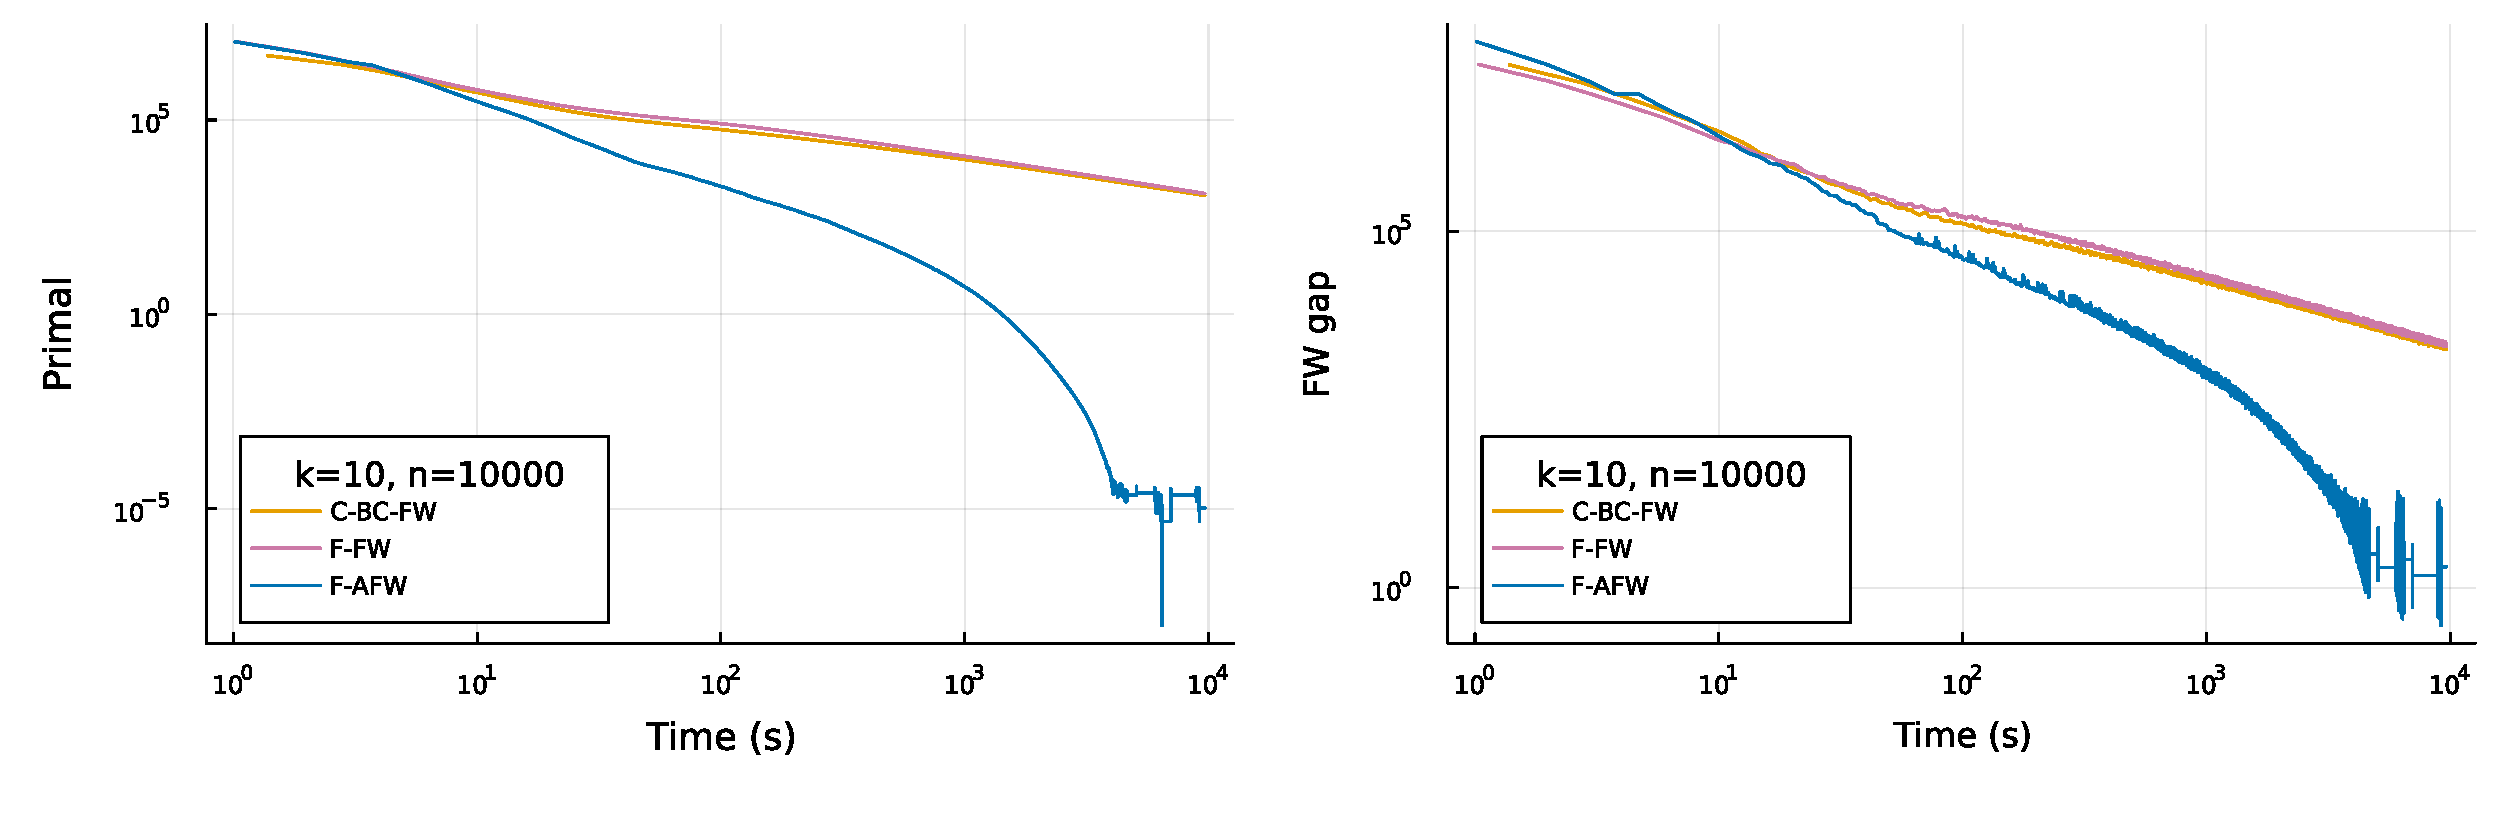
\includegraphics[width=0.98\textwidth]{./figures/plot_ni_k10_n10000_npub20000_unif_i10000_s240389_cvxho-mat_a-p1_p2_segment-0.5_ref-vertex_t20260328_082154}
%\end{adjustbox}
\caption{%C-BC-FW, F-FW, and F-AFW
FW variants, run for up to $10\,000$ iterations on ten non-intersecting point-cloud polytopes in $\R^{10\,000}$.}
\label{fig:k10n10000_pc_ni}
\end{figure*}

\begin{figure*}[!t]
\centering
%\hspace*{-0.075\textwidth} % Shift the image 5% of the text width to the left
%\begin{adjustbox}{center}
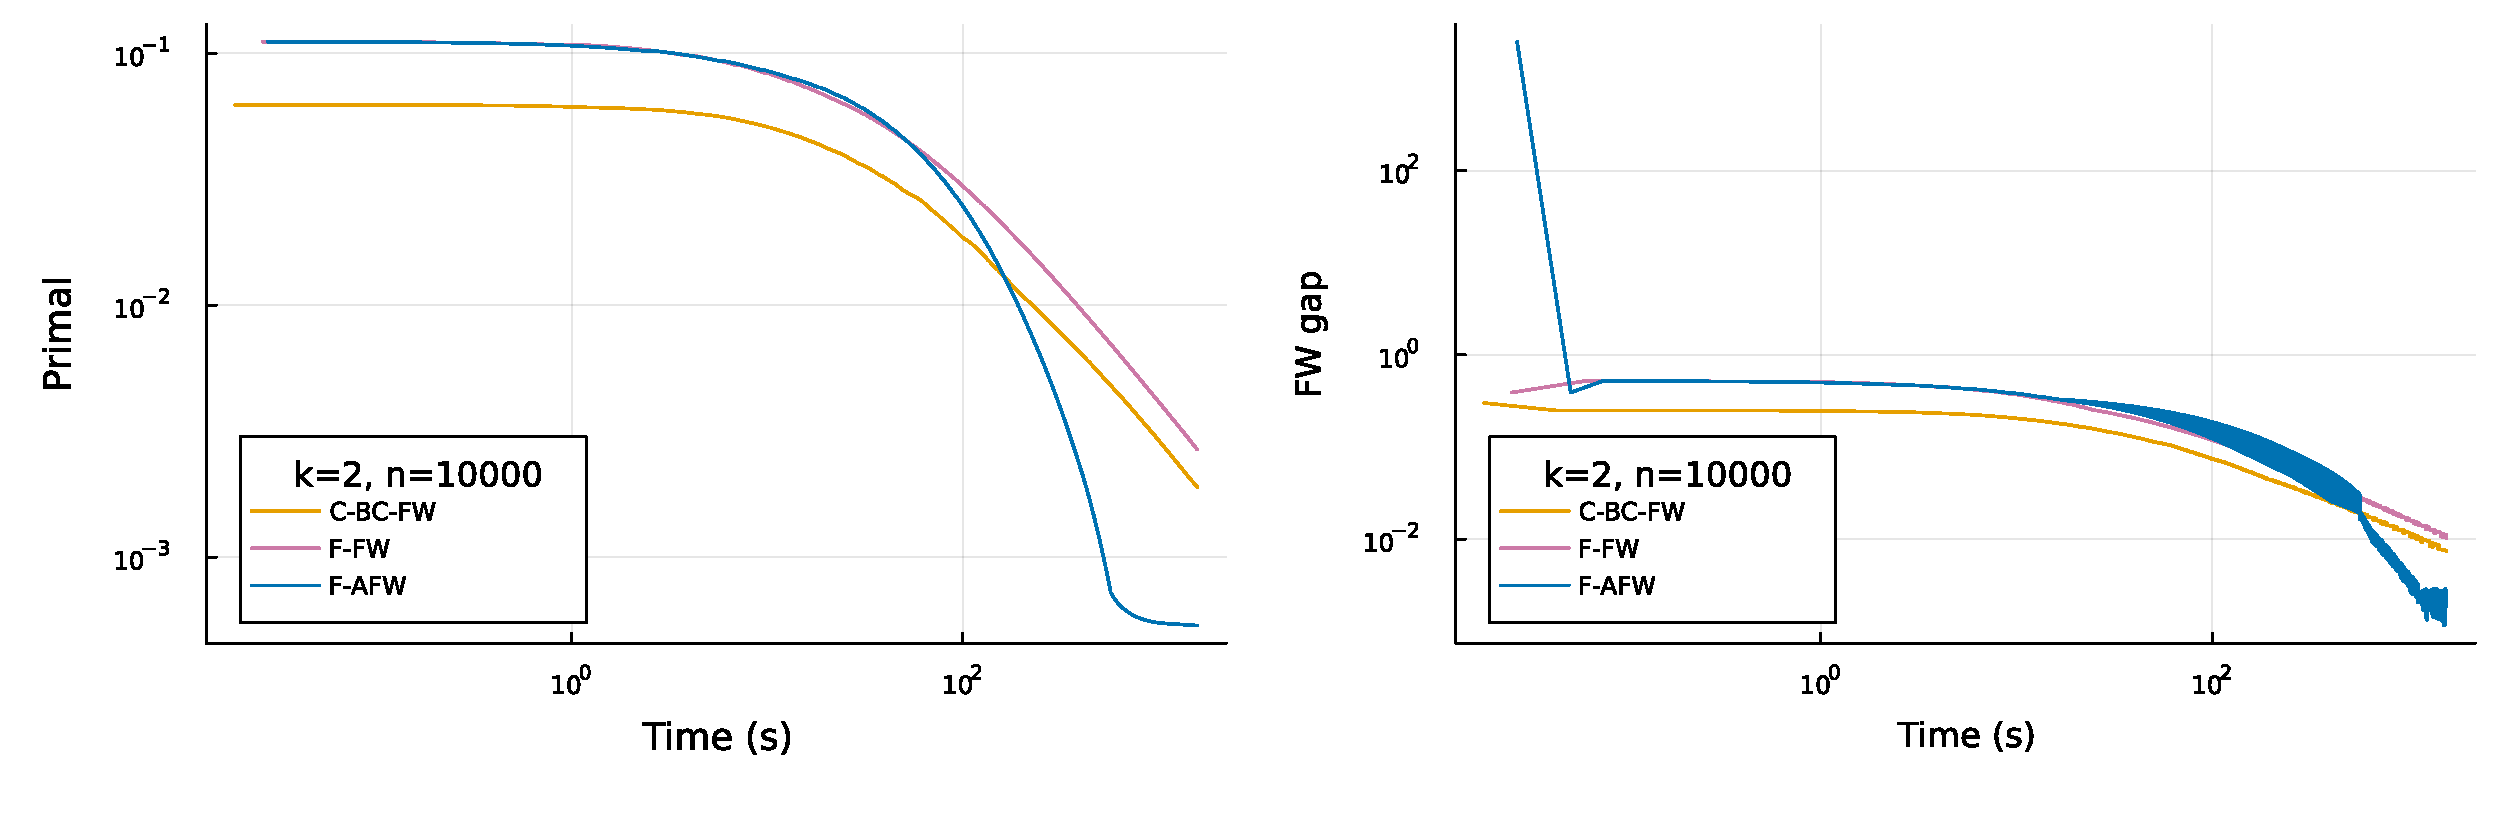
\includegraphics[width=0.98\textwidth]{./figures/plot_i_vf_k2_n10000_i80000_s42_a0p1_b0p3_d0p45_tp-mid_sep-0p5_t20260324_022349}
%\end{adjustbox}
\caption{%C-BC-FW, F-FW, and F-AFW
FW variants, run for up to $80\,000$ iterations on two intersecting vertex-facet polytopes in $\R^{10\,000}$.}
\label{fig:k2n10000_vf_i}
\end{figure*}

\begin{figure*}[!t]
\centering
%\hspace*{-0.075\textwidth} % Shift the image 5% of the text width to the left
%\begin{adjustbox}{center}

\includegraphics[width=0.98\textwidth]{./figures/plot_i_k2_n20000_i1000_s240389_cvxho_anc_t20250511_212230_fromlogs}
%\end{adjustbox}
\caption{%C-BC-FW, F-FW, and F-AFW
FW variants, run for up to $1\,000$ iterations on the two polytopes from \cref{fig:k2n20000_pc_ni}, translated to intersect.}
\label{fig:k2n20000_pc_i}
\end{figure*}


Each instance is constructed by generating $k$ polytopes.
Here we report results for settings with $k = 2, 10$ polytopes in $\R^n$, with up to $n = 20\,000$. We present more plots, corresponding to additional setups in \cref{a:extra_experiments}. 
%vertices per polytope. 
We generate two kinds of problems: one where the polytopes do not intersect (cf. \cref{fig:k2n20000_pc_ni,fig:k10n10000_pc_ni}) and another where they do (cf. \cref{fig:k2n20000_pc_i,fig:k2n10000_vf_i}). 
\gabaistats{Moreover, we test two polytope setups, that we call ``point-cloud'' and ``vertex-facet'' throughout.}
In the point-cloud setup \gabaistats{(cf. \cref{fig:k2n20000_pc_ni,fig:k10n10000_pc_ni,fig:k2n20000_pc_i})}, each polytope is generated as the convex hull of a list of points that are sampled uniformly at random from mutually disjoint intervals for every coordinate $i \in [n]$.
%\Dav{maybe point to the slides of sebastian's paper that did the same to generate polytopes. But maybe not, it'd be a weird thing to reference }
%\dav{``Further, we note that, for all instances, we compute \LMO{}s that perform a single linear pass over the point list, evaluating one dot product per point.'' DM: if you want to add this detail, do it in the appendix}
For each polytope, we draw the number of points uniformly at random in $[n, 2n]$. This choice keeps each polytope ``reasonably challenging'' to optimize over.
%, while ensuring that the cost of the oracle remains manageable for all runs. 
In \cref{a:extra_experiments}, we also report an example with two disjoint polytopes in $\R^{10\,000}$ built from $100\,000$ vertices, an order of magnitude larger: the convergence behavior of the tested algorithms in that instance is essentially unchanged, and only the absolute time to convergence increases, reflecting a higher cost for the \LMO{}.
%We then computed the convex hull of these points to form each polytope.\dav{but how many vertices do you have then in the end for the polytope? people are going to wonder}
\gabaistats{In the vertex-facet setup (cf. \cref{fig:k2n10000_vf_i}), we only consider the case $k =2$, and the polytopes are generalizations of an $\ell_\infty$-ball and of an $\ell_1$-ball, respectively.}
%In the latter case, 
Then, we shift the aforementioned polytopes %$\mP_1, \mP_2, \dots, \mP_k$
so they 
% have one vertex in common, ensuring a non-empty intersection.
have non-empty intersection. 
Concretely, \gabaistats{in the point-cloud setup} we shift $\mP_2$ until one of its vertices coincides with a vertex $v$ of $\mP_1$; we then move $\mP_2$ towards the barycentre of $\mP_1$ (the average of its vertices); finally, we translate all remaining polytopes so they share $v$. 
\gabaistats{Instead, in vertex-facet intersections only a single vertex of the generalized $\ell_1$-ball touches the interior of a facet of the generalized $\ell_\infty$-ball.}

Our experiments compare the \FW{} and \AFW{} algorithms, cf. \cref{a:algos}, with different heuristic variants. 
% For each, \FW{} and \AFW, We implement three types of algorithms: (1) ``full'' (F-\FW{} and F-\AFW{}), that at each iteration computes a single \LMO{} over the entire product polytope $\mP$ and maintains a single \emph{active set} in the product, which is a set of previously computed extreme points stored such that the current iterate can be written as a convex combination of such points, (2) ``full block-coordinate'' (F-BC), where we also compute the full \LMO{} but treat each component independently with a separate active set to represent the variable for that component, and (3) ``cyclic block-coordinate'' (C-BC) where at each iteration we only compute the \LMO{} of one component and update the corresponding variable only.
We implement two types of algorithms: ``full'' (F-\FW{} and F-\AFW{}), that at each iteration computes a single \LMO{} over the entire product polytope $\mP$ and maintains a single \emph{active set} in the product - i.e., a set of previously computed extreme points stored such that the current iterate can be written as a convex combination of such points - and ``cyclic block-coordinate'' (C-BC), where at each iteration we only compute the \LMO{} of one component and update the corresponding variable and active set only.
% In particular, in the full block-coordinate approach (F-BC-FW, F-BC-AFW), all $k$ \LMO{}s are evaluated independently and in parallel in each iteration\dav{note here that F-FW is the same as F-BC-FW since FW doesn't have an active set and say that because of this, we do not have one of those algorithms in the plots and do that}. The product of these solutions is an \LMO{} for the product, but we note that the block-coordinate AFW algorithm stores and uses the so-called away vertices \textit{for each polytope}, as opposed to the full AFW that directly works with the product polytope.
%On the other hand, in the cyclic block-coordinate regime (C-BC-\FW{}), the variables corresponding to each block are updated sequentially. 
%To our knowledge, the only existing competitive FW-based method for the set-intersection problem is \cref{algo:alm} from \citep{BPW23}, which implements exactly C-BC-FW for the case $k=2$. % this is something for the related work.
At each iteration $t$, F-\AFW{} optimizes over the active set to find an away vertex, and updates the set, see \cref{algo:AFW}. 
An away vertex $a_t$ allows the algorithm to choose to move in the direction guaranteeing more progress, namely, taking an \emph{away step} from $x_t$ in the direction $x_t - a_t$, or taking a \emph{\FW{} step} from $x_t$ towards the \LMO{} solution.
% In these two phases, active set optimization and update, F-BC-\AFW{} exploits the feasible set structure through block decompositions and block updates.

All algorithms were run with a standard line search, see \cref{a:algos}.
%\dav{Gabriele, the line search is not specified or discussed in \cref{a:algos} and it should}
%In the short-step setting, the step-size is determined using the smoothness constant $L = 2$, as established in \cref{prop:lsmooth_cvx_pl_intersection_k}. 
\gabaistats{For each experimental setup, we ran every \FW{} variant until the \FW{} gap dropped below $1e-07$ or until a setup-specific iteration budget was reached, whichever occurred first. }

In the plots, we report the following metrics to quantify algorithmic performance over iterations: the primal gap $f(x_t)-\min_{x\in\mP}f(x)$, and also the so-called \FW{} gap $\max_{x \in \mathcal{P}} \innp{\nabla f(x_t), x_t - x}$ \citep{BCC+23}. 
While the former cannot be calculated in general, since one does not usually know the minimum objective value a priori, the latter is a standard measure for \FW{} algorithms, since it is an upper bound on the former while at the same time being computable.
Therefore, the \FW{} gap results in a stopping criterion that can be used to guarantee $\epsilon$-optimality has been reached.
We thus used it as a stopping criterion in our experiments, if they already converged, cf. \citep{Jag13}.
Both metrics in the figures below are plotted against
%recorded as functions of the iteration count and as a function of
the elapsed wall-clock time, in seconds, \gabaistats{measured within the corresponding \FW{} routine, using logarithmic scales on both axes.}

\gabaistats{Note that the \FW{} gap is not guaranteed to decrease monotonically but its minimum across iterations decreases linearly, see the plots.
Furthermore, we remark that small non-monotonic fluctuations of the primal gap in the tail of \cref{fig:k10n10000_pc_ni} are numerical artifacts caused by finite-precision effects and the approximate computation of the reference optimum.}

The implementation was carried out fully in Julia (Version 1.9.4) and, in particular, we relied on the \href{https://github.com/ZIB-IOL/FrankWolfe.jl}{\texttt{FrankWolfe.jl}} package (Version 0.5.0, MIT License) for the algorithmic part.
All runs were executed on Slurm compute nodes equipped with Intel Xeon Gold 6\,342 processors, each providing 96 logical cores, and approximately 512GiB RAM, interconnected via Infiniband.
We requested $k$ cores per task in Slurm via \texttt{\#SBATCH\ --cpus-per-task=k}, and then set \texttt{export JULIA\_NUM\_THREADS=\$SLURM\_CPUS\_PER\_TASK} so that Julia's \FW{} routines used exactly $k$ threads.
The code for reproducing the results in this section \gabaistats{is available at TODO: URL}.% will be made publicly available upon publication and can be found in the supplementary material.

% \cref{fig:k2n20000,fig:k2n20000_pc_ni} showcase the superiority of the block-coordinate implementations over the traditional full-product approaches, as well as the benefits of employing \AFW{} variants, in speeding up convergence.
% Notably, our computational results provide empirical confirmation of the our theoretical linear rates for \AFW{} in several scenarios, converged consistently faster than F-\FW{}, F-BC-\FW{} and C-BC-\FW{}, in all settings, on disjoint polytopes.
%
%We found a consistent hierarchy across all experimental settings. F‑BC‑\AFW{} is always fastest, even in the most challenging case with ten polytopes, see \cref{fig:k2n20000_pc_ni}. F‑\AFW{} is the runner-up, even though its advantage over the remaining methods considerably decreases as $k$ increases, especially in terms of FW gap, cf. \cref{fig:k5n10000} and \cref{fig:k2n20000_pc_ni}.  Even as the number of polytopes grows, \AFW{} maintains a clear edge over the other variants, although this advantage gradually diminishes, particularly in terms of the measured \FW{} gap. 
All in all, we found a consistent hierarchy across all experimental settings. 
We observe that the full \AFW{} variant enjoys the best performance among the tested algorithms:
%, although the underlying theoretical analysis and linear rates remain invariant\dav{not true! we only have theory for the F-AFW algorithm} for F-\AFW{} and F-BC-\AFW{}, 
% This is likely due to F-BC-\AFW{} having an improved management of the active set. At each iteration $t$, \AFW{} optimizes over the active set, to find an away vertex, and updates the set, see \cref{algo:AFW}. 
\gabaistats{away steps not only accelerate the algorithm in practice in high-dimensional product polytope setting, }
%This not only accelerates the algorithm in practice in high-dimensional settings,
but are key for our linear convergence analysis, as the plots show.
% F‑BC-\AFW{} is always fastest, even in the most challenging case with ten polytopes, see \cref{fig:k2n20000_pc_ni}. F‑\AFW{} is the runner-up, even though its advantage over the remaining methods considerably decreases as $k$ increases, especially in terms of FW gap, cf. \cref{fig:k5n10000} and \cref{fig:k2n20000_pc_ni}.
Even as 
%the number of polytopes grows,
$k$ and $n$ grow, \AFW{} maintains a clear edge over the other variants\gabaistats{, although
%this advantage gradually diminishes, particularly in terms of the measured \FW{} gap. 
a larger iteration budget is needed for the linear regime to emerge.}
% The \FW{}-based variants have similar performance, with F‑BC‑\FW{} coming third, and  F‑\FW{} and C‑BC‑\FW{} performing the worst. 
Instead, the algorithmic performance of the tested \FW{}-based variants F-\FW{} and C-BC-\FW{} is very similar, and it yields worse convergence than F-\AFW{}. 
Surprisingly, on our instances, the cyclic block‑coordinate \FW{} strategy offers no practical gain over the full \FW{} variant, even with large $k$.

% For the case of intersecting polytopes in \cref{fig:k2n10000_pc_i} and others in \cref{a:extra_experiments}, the problem becomes easier and the difference among algorithms becomes narrower.
% We also note that the convergence happens to be faster across all algorithms for the non-intersecting setting.
% Compare \cref{fig:k2n10000_pc_i}, reporting algorithmic performances on the same polytopes used in \cref{fig:k2n20000_pc_ni} but made to intersect, and see the experiments in \cref{a:extra_experiments}, where we showcase more problems with non-empty intersection.
\gabaistats{
For the intersecting point-cloud instances, the empirical separation among the algorithms appears less pronounced than in the non-intersecting case.
In particular, comparing \cref{fig:k2n20000_pc_i}, reporting algorithmic performances on the same polytopes used in \cref{fig:k2n20000_pc_ni} but translated so as to create a non-empty intersection, we observe that the curves in the intersecting case are closer to each other, suggesting a smaller performance gap.
%Since these instances are obtained by translation, this effect should not be attributed to a change in global domain-geometric quantities such as the pyramidal width of the product polytope.
In these instances, a high-dimensional intersection yields a high-dimensional optimal set containing many points.
This can make optimal-face identification less effective in practice. It is also is consistent with less favorable local conditioning near the attained optimum, say on the optimal face, which plausibly reduces the empirical advantage of \AFW{} over \FW{}.

By contrast, in the vertex-facet construction the intersection is a single point by design, so the optimal set is isolated and the associated optimal face is geometrically much ``sharper''.
In this setting, a larger face-dependent pyramidal-width-type constant is consistent with the clearer linear regime observed for \AFW{}.

Additional examples showing similar behavior are reported in \cref{a:extra_experiments}.
We also note that the convergence happens to be faster across all algorithms for the non-intersecting, point-cloud setting.
}

% We remark that, although exact line search ensures a nonincreasing primal gap (see \cref{a:algos}), our plots exhibit slight oscillations near convergence. These slight perturbations are due to minor numerical errors in the \texttt{Goldenratio} line search implementation in the \texttt{FrankWolfe.jl} package, that we chose for our runs, where finite‐precision (\texttt{Float64}) rounding can introduce small errors. In practice, these minor oscillations do not change the overall convergence pattern, which still aligns with theoretical guarantees.
%
We note that we also experimented with a stochastic block-coordinate \FW{} variant, which differs from C-BC-\FW{} by selecting blocks in random order instead of cyclically. In our tests, its primal and FW gap trajectories were almost exactly the same as those of C-BC-\FW{}, so we decided to omit it from our figures.

%\cref{fig:k2n20000,fig:k2n20000_pc_ni}
The plots showcase the superiority of
%the block-coordinate implementations over the traditional full-product approaches, as well as the benefits of
employing \AFW{} variants in speeding up convergence.
Most importantly, \emph{our computational results provide empirical confirmation of our theoretical linear rates for \AFW{}} in several scenarios, as this algorithm converged \gabaistats{at least as fast, and often} consistently faster, than F-\FW{}
%, F-BC-\FW{}
and C-BC-\FW{} in all settings.% on disjoint polytopes.

\section{Conclusion}

In this work, we have shown that the product of well‐conditioned polytopes inherits a robust notion of conditioning, both in terms of pyramidal width and vertex–facet distance, which in turn guarantees linear convergence of the Away Frank-Wolfe method under standard assumptions.

Our analysis yields explicit bounds on the resulting condition numbers of the product domain, and thus on the convergence rate, as a function of the individual polytope components.

We then applied this theory to the classical convex-feasibility problem over intersections of polytopes by minimizing a smooth, convex, Polyak-Łojasiewicz objective over the Cartesian product. We provided empirical results that strongly corroborate our findings.

% ------------------------------
\section*{Acknowledgements}
The research in this paper was partially supported through the Research Campus Modal funded by the German Federal Ministry of Education and Research (fund numbers 05M14ZAM,05M20ZBM) and the Deutsche Forschungsgemeinschaft (DFG) through the DFG Cluster of Excellence MATH+.
David Martínez-Rubio was partially funded by the project IDEA-CM (TEC-2024/COM-89).
Francisco Criado was supported by grant PID2022-137283NB-C21.


\clearpage
%\vspace{2cm}
\printbibliography[heading=bibintoc] %


%{\small
%%\bibliographystyle{unsrt}%apalike%splncs04
%\bibliographystyle{apalike}%apalike%splncs04
%\bibliography{biblio_giommazz}
%}



















%%%%%%%%%%%%%%%%%%%%%%%%%%%%%%%%%%%%%%%%%%%%%%%%%%%%%%%%%%%%
\clearpage
\section*{Checklist}


% %%% BEGIN INSTRUCTIONS %%%
% The checklist follows the references. For each question, choose your answer from the three possible options: Yes, No, Not Applicable.  You are encouraged to include a justification to your answer, either by referencing the appropriate section of your paper or providing a brief inline description (1-2 sentences). 
% Please do not modify the questions.  Note that the Checklist section does not count towards the page limit. Not including the checklist in the first submission won't result in desk rejection, although in such case we will ask you to upload it during the author response period and include it in camera ready (if accepted).

% \textbf{In your paper, please delete this instructions block and only keep the Checklist section heading above along with the questions/answers below.}
% %%% END INSTRUCTIONS %%%


\begin{enumerate}

\item For all models and algorithms presented, check if you include:
  \begin{enumerate}

\item A clear description of the mathematical setting, assumptions, algorithm, and/or model.

[Yes]
Notation is described in \cref{s:preliminaries}. All assumptions on convexity, smoothness and the Polyak–Łojasiewicz condition, listed in \cref{s:preliminaries}, are stated in our linear convergence theorems appearing in \cref{s:convergence}. The minimal hypotheses on the polytopes whose condition numbers we examine appear in \cref{s:conditioning_convergence}. All of the full proofs are given in \cref{a:proofs}, except for the very short one of \cref{cor:affinepyr_sameas_pyr}, that is located in the main paper.
The examined Frank–Wolfe variants are described in \cref{a:algos}.


\item An analysis of the properties and complexity (time, space, sample size) of any algorithm.

[Yes]
We analyze linear convergence rates for Away-FW over product polytopes under PL, with rates expressed via the polytope condition numbers known as pyramidal width and the vertex–facet distance. Notably, we quantify these condition numbers for product polytopes and connect them to iteration complexity in \cref{s:conditioning_convergence}, \cref{s:polytope_intersection}, \cref{a:linconv_pw}, and \cref{a:linconv_vfd}.

\item (Optional) Anonymized source code, with specification of all dependencies, including external libraries.

[Yes]
The data and code is available in the supplementary material. We will publish all code, data, and logs in a publicly accessible GitHub repository, including (i) the complete \texttt{Julia} package source for generating instances and running the experiments (including \texttt{Project.toml} and \texttt{Manifest.toml} files pinning all dependency versions), fully commented to assist both expert and beginner users in understanding the code, (ii) all \texttt{.CSV} logs used to generate the paper's plots, alongside scripts for parsing and plotting, (iii) comprehensive \texttt{README} files with step-by-step instructions for installing the package, reproducing the experiments both locally or on a SLURM-managed server, and re-generating all plots.

\end{enumerate}

\item For any theoretical claim, check if you include:
\begin{enumerate}
\item Statements of the full set of assumptions of all theoretical results.

[Yes]
Assumptions on convexity, smoothness, PL condition, and polytope structure are stated with each result; see \cref{s:preliminaries}, \cref{s:conditioning_convergence}, and \cref{s:polytope_intersection}
\item Complete proofs of all theoretical results.

[Yes]
Full proofs appear in \cref{a:proofs}. The short proof of \cref{cor:affinepyr_sameas_pyr} is kept in the main text.
\item Clear explanations of any assumptions.

[Yes] Assumptions are motivated and discussed alongside the main theorems and their proofs.
\end{enumerate}

\item For all figures and tables that present empirical results, check if you include:
\begin{enumerate}
\item The code, data, and instructions needed to reproduce the main experimental results (either in the supplemental material or as a URL).

[Yes]

\cref{s:experiments} and \cref{a:extra_experiments} describe dataset generation, parameter settings ($k$, $n$, maximum number of iterations for the tested algorithms, their step size strategy and termination criterion), and the hardware and software environment. 
In particular, all datasets are synthetically generated with the procedure described in the paper, and more documentation can be found directly in the code. The full code to reproduce these experiments will be made available upon publication and is attached in the supplementary material.
The manuscript also includes pseudocode in \cref{a:algos}. 
\item All the training details (e.g., data splits, hyperparameters, how they were chosen).

[Yes]
We report the experimental-configuration details that serve as training details for optimization studies: (i) instance-generation protocols for intersecting and disjoint product polytopes, with all parameter values and random seeds; (ii) algorithmic hyperparameters for each Frank–Wolfe variant, including step-size policy and away-step selection; (iii) stopping criteria (maximum iterations and Frank–Wolfe gap threshold); and (iv) software/hardware environment. Because instances are synthetically generated, train/validation/test splits are not applicable; comparability is ensured via fixed seeds and replicated runs. See \cref{s:experiments} and \cref{a:extra_experiments}.
\item A clear definition of the specific measure or statistics and error bars (e.g., with respect to the random seed after running experiments multiple times).

[Yes]
We quantify run-to-run variability by including additional plots, pertaining to instances generated with different random seeds, in \cref{a:extra_experiments}. These supplementary figures closely mirror the behavior of the tested algorithms that is already shown in the main paper, and confirm our theoretical findings. This approach, namely, providing additional figures which plot performance curves across multiple seeds, serves the purpose of confirming the statistical significance of our claims.

\item A description of the computing infrastructure used. (e.g., type of GPUs, internal cluster, or cloud provider).

[Yes]
Experiments were run on SLURM-managed nodes with Intel Xeon Gold 6\,342 CPUs (96 logical cores) and \mbox{$\sim$512\,GiB} RAM over InfiniBand; we specify threading and SLURM settings (\texttt{cpus-per-task} and \texttt{JULIA\_NUM\_THREADS}) in \cref{s:experiments}.
\end{enumerate}

\item If you are using existing assets (e.g., code, data, models) or curating/releasing new assets, check if you include:
\begin{enumerate}
\item Citations of the creator If your work uses existing assets.

[Yes]
We cite \texttt{FrankWolfe.jl} and all prior theoretical results underpinning our analysis.
\item The license information of the assets, if applicable.

[Yes]
We state that the \texttt{FrankWolfe.jl} is MIT license and include license details for any external packages used.
\item New assets either in the supplemental material or as a URL, if applicable.

[Yes]
We release an anonymized code archive in the supplementary material. A public repository will be posted on GitHub upon publication with code, logs, and scripts.
\item Information about consent from data providers/curators.

[Not Applicable]
All data are synthetic and generated as described. No external providers or human data are involved.
\item Discussion of sensible content if applicable, e.g., personally identifiable information or offensive content.

[Not Applicable]
The work contains no sensitive content or personally identifiable information. Synthetic instances contain only randomly generated numeric data.
\end{enumerate}

\item If you used crowdsourcing or conducted research with human subjects, check if you include:
\begin{enumerate}
\item The full text of instructions given to participants and screenshots.

[Not Applicable]
The paper involves no crowdsourcing or human subjects.
\item Descriptions of potential participant risks, with links to Institutional Review Board (IRB) approvals if applicable.

[Not Applicable]
No human studies were conducted.
\item The estimated hourly wage paid to participants and the total amount spent on participant compensation. 

[Not Applicable]
No participants were recruited.
\end{enumerate}

\end{enumerate}



\clearpage
\appendix
\thispagestyle{empty}

% Supplementary material: To improve readability, you must use a single-column format for the supplementary material.
\onecolumn
\aistatstitle{Supplementary Material}

% --------------------
\section{Proofs}\label{a:proofs}

% --------------------
\subsection{Pyramidal width}\label{a:pw}

\cref{fact:cart_prod_kpolytopes} contains some simple known facts about polytopes, that serve as a warm-up and will be useful in the sequel.

\begin{lemma}[\textbf{Cartesian product of $k$ polytopes}]\label{fact:cart_prod_kpolytopes}
The Cartesian product $\mP = \Pi_{i \in [k]} \mP_i$ of $k$ polytopes, each in $\R^n$ for some $n \in \mathbb{N}_{>0}$, is a polytope of dimension $kn$.
In particular, $\verts{\mP} = \Pi_{i \in [k]}\verts{\mP_i}$.
Further, if $F_\mP \in \faces{\mP}$, then  $F_\mP$ is the product of faces of all the individual polytopes, i.e., $\forall i \in [k]$ there exist $F_{\mP_i} \in \faces{\mP_i}$ such that $F_\mP = \Pi_{i \in [k]} F_{\mP_i}$.
\end{lemma}

\begin{proof}
For all $i \in [k]$, we denote the $i$-th polytope by $\mP_i \defi \{x \in \R^n : A_{\mP_i} x \le b_{\mP_i}\}$, where $A_{\mP_i} \in \R^{m_{\mP_i} \times n}$ and $b_{\mP_i} \in \R^{m_{\mP_i}}$. 
Compactness and convexity are inherently preserved in the Cartesian product, so
\[
\begin{array}{rcl}
\Pi_{i \in [k]} &=& \{(x^1, \dots, x^k) \in \R^n\times\cdots \times\R^n\,:\, x^1 \in \mP_1, \dots, x^k \in \mP_k\}\\
&=& \{(x \in \R^{kn}\,:\, \forall i \in [k]\,,\, A_{\mP_i} x^i \le b_{\mP_i}\}\,.
\end{array}
\]
By linearity of the constraints and independence of each block $i \in [k]$,
%of constraints only involves one polytope at a time,
% \[
% \mP_1 \times \cdots \times \mP_k = \left\{x \in \R^{kn} \,:\: 
% \left(\begin{array}{cccc}
% A_{\mP_1} & 0 & \cdots & 0 \\
% 0 & A_{\mP_2} & & \vdots \\
% \vdots & & \ddots & 0 \\
% 0 & \cdots & 0 & A_{\mP_k} \\
% \end{array}\right)
% \begin{pmatrix}
%     x_1\\
%     \vdots\\
%     x_k
% \end{pmatrix} \le \begin{pmatrix}
%     b_{\mP_1} \\
%     \vdots\\
%     b_{\mP_k}
% \end{pmatrix}\right\}\,,
% \]
the product is still a polytope described by a constraint matrix in $\R^{(m_{\mP_1}+\dots+m_{\mP_k})\times kn}$ with diagonal blocks $A_{\mP_i}$, for $i \in [k]$, and right-hand side coefficients $b_{\mP_i} \in \R^{m_{\mP_1}+\dots+m_{\mP_k}}$.
Moreover, since $\forall i \in [k]$, $\mP_i = \conv{\mP_i}$ and $\conv{\Pi_{i \in [k]}\mP_i} = \Pi_{i \in [k]}\conv{\mP_i}$, then $\verts{\mP} = \Pi_{i \in [k]}\verts{\mP_i}$.
% We show that the lemma is valid for two polytopes $\mP$ and $\mQ$. 
% Denote by $\text{conv}(\verts(\mP)$ and $\text{conv}(\verts(\mQ)$ the convex hull of $\mP$ and $\mQ$, respectively, and by $\Delta_{n-1}$, is given by $\Delta_{n-1} = \{z \in \R^n : z_i \ge 0, \text{ for } i \in [n],\, \|z\|_1 = 1\}$ the standard $(n-1)$-simplex.
% We use the definition of polytopes as the convex hull of their vertices, i.e., $\mP = \text{conv}(\verts(\mP)$ and $\mQ = \text{conv}(\verts(\mQ)$, and $\mP \times \mQ = \text{conv}(\verts(\mP) \times \text{conv}(\verts(\mQ)$. So
% \begin{equation}
% (x,y) = \left(\sum_{i=1}^{|\verts(\mP|} \lambda_i v_i, \sum_{j=1}^{|\verts(\mQ|} \mu_j w_j\right) \in \text{conv}(\verts(\mP) \times \text{conv}(\verts(\mQ)\,,
% \label{eq:convconv_mPmQ}
% \end{equation}
% for $v_i \in \verts(\mP$, $w_j \in \verts(\mQ$, $\lambda, \mu \in \Delta_{n-1}$. We will show that $\text{conv}(\verts(\mP) \times \text{conv}(\verts(\mQ) = \text{conv}\left(\verts(\mP \times \verts(\mQ\right)$.
% If $(x',y') \in \text{conv}\left(\verts(\mP \times \verts(\mQ\right)$, then $(x',y') = \sum_{i=1}^{|\verts(\mP|}\sum_{j=1}^{|\verts(\mQ|} \gamma_{ij} (v_i, w_j)$, where $\gamma \in \Delta_{|\verts(\mP| + |\verts(\mQ| - 1}$.
% Expanding and summing over the appropriate indices yields $(x',y') = (\sum_{i=1}^{|\verts(\mP|}v_i \sum_{j=1}^{|\verts(\mQ|}\gamma_{ij}, \sum_{j=1}^{|\verts(\mQ|}w_j \sum_{i=1}^{|\verts(\mP|}\gamma_{ij})$, where each $\sum_{i=1}^{|\verts(\mP|}\sum_{j=1}^{|\verts(\mQ|}\gamma_{ij}$ sums up to 1, thus contributing to a convex combination within $\mP$ and $\mQ$, based on their respective indices. Renaming the sums as $\sum_{j=1}^{|\verts(\mQ|}\gamma_{ij} = \lambda_i$ and $\sum_{i=1}^{|\verts(\mP|}\gamma_{ij} = \mu_j$ for clarity, we get \cref{eq:convconv_mPmQ} indicating that $\text{conv}(\verts(\mP \times \verts(\mQ)$ is equivalent to $\text{conv}(\verts(\mP) \times \text{conv}(\verts(\mQ)$, thus completing the proof.
% Extending this proof to encompass $k$ polytopes employs the same steps, albeit with heavier notation, so we skip it here for ease of readability. 
Finally, a polytope face is the set of points optimizing some linear functional over the polytope.
Consider the linear functional defined by $n = (n^1, \ldots, n^k) \in \R^k$.
A point $(p^1, \ldots, p^k) \in \mP$ optimizes the linear functional defined by $n$ if and only if, each $p^i$ optimizes the linear functional defined by the corresponding $n^i$ over $\mP_i$, as a linear program in the product is solved in each component independently. 
If, for all $i \in [k]$, we denote the faces defined by that condition as $F_i \subseteq \mP_i$, the set of points optimizing $n$,is exactly $F_1 \times F_2 \times \cdots \times F_k \subset \mP_1 \times \mP_2 \times \cdots \times \mP_k$, i.e., a face $F_\mP$ of $\mP$.
\end{proof}


\begin{proof}\linkofproof{lemma:affine_pyramidal_width}

Suppose that $p$ is not in the relative interior of $f$. Then $p$ might be in the exterior or in the boundary of $f$.
%
Choose one facet $g$ of $f$ such that $\aff{g}$ separates
$p$ from the interior of $f$ ($p$ could lie exactly in $\aff{g}$ if $p$ is in the relative boundary of $f$). We will show that $\whatface{g}{\mP}<\whatface{f}{\mP}$, which would be a contradiction.

\begin{figure}[ht!]
\centering
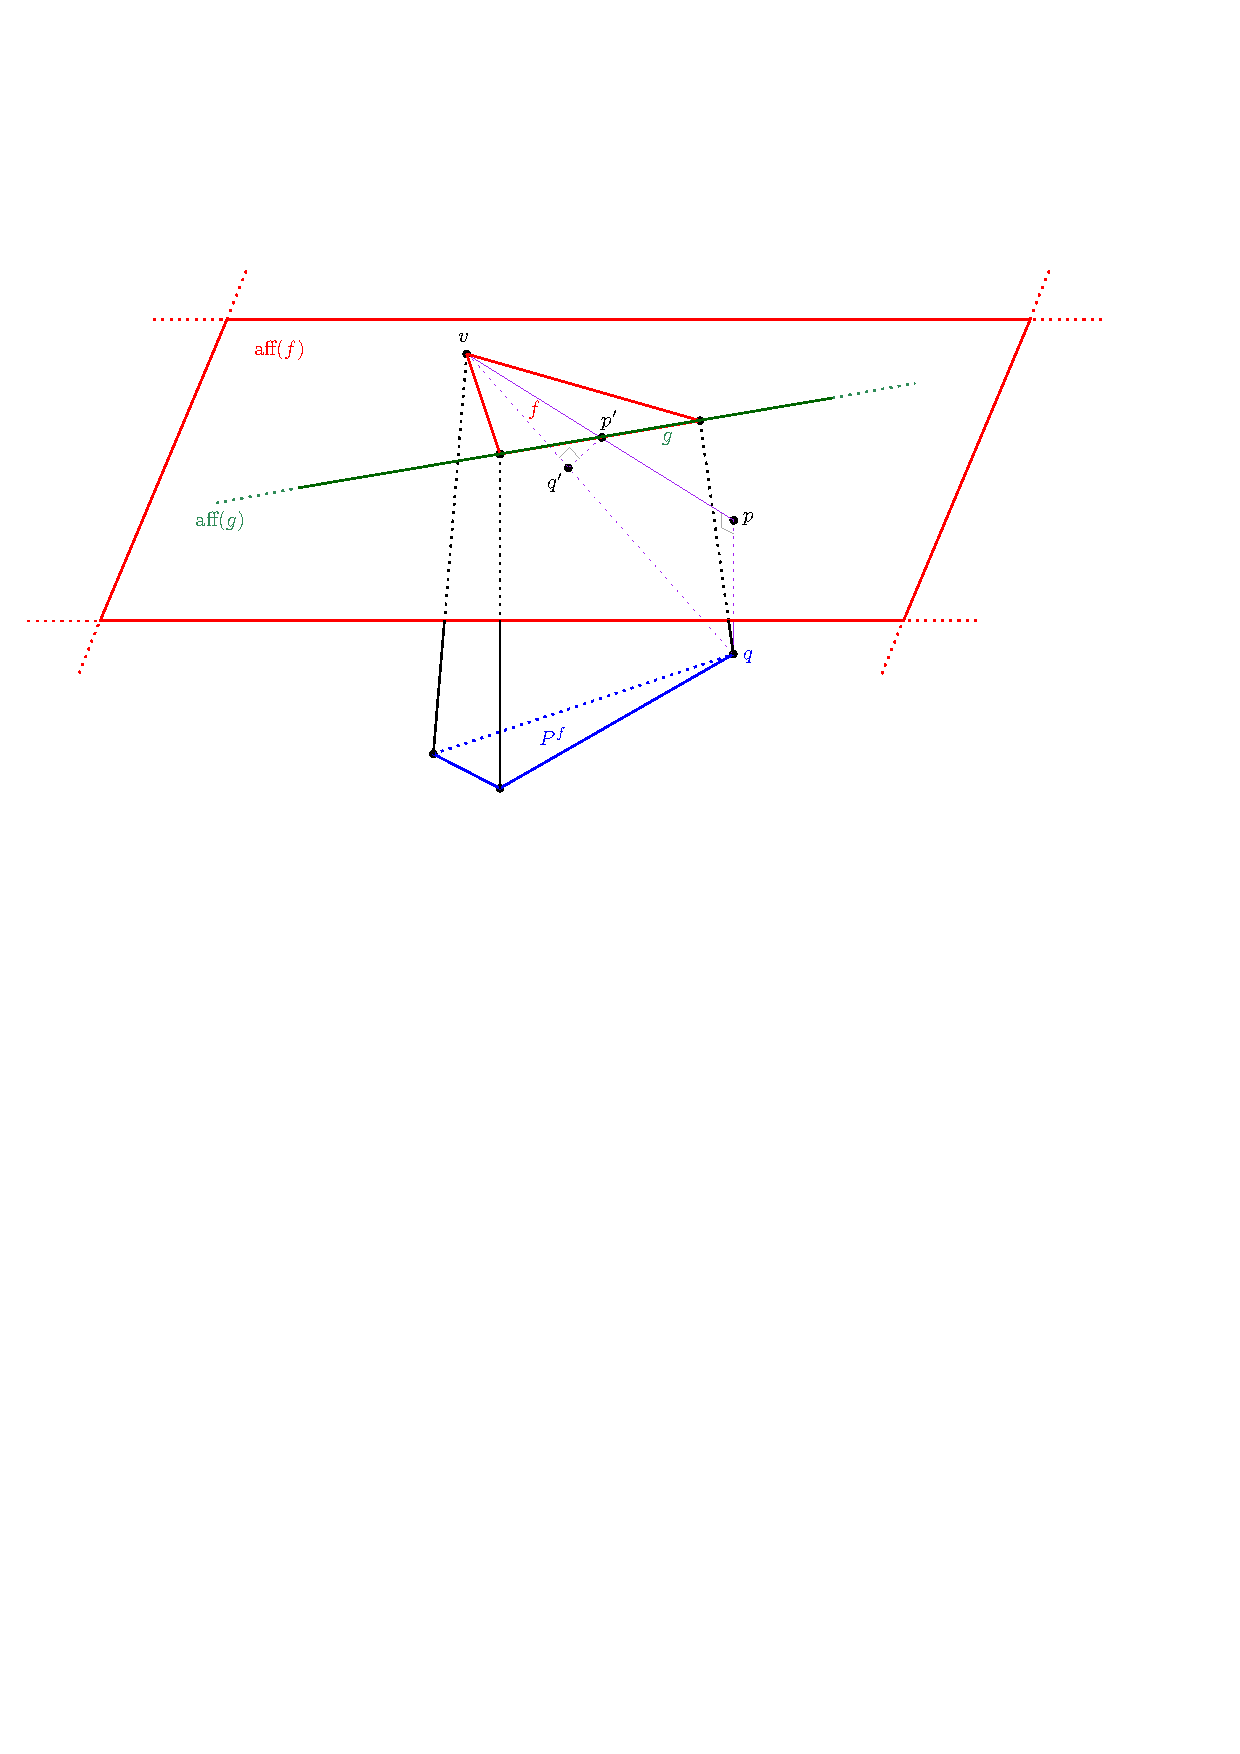
\includegraphics[width=0.8\textwidth]{figures/bpcg.pdf}
\caption{\gabrev{To prove that $\dist{\aff{g}, [q,v]} < \dist{\aff{f},q}$, we looking at the right triangle $v,p,q$ and compare $\dist{p',q'}$ with $\dist{p,q}$.}
% We are proving that $\dist{\aff{f},q}>\dist{\aff{g}, [q,v]}$ In the right triangle $v,p,q$, we are comparing $\dist{p',q'}$ with $\dist{p,q}$. Observe that the triangle $v,p,q$ is a right triangle and $\dist{p', q'}$ is at most the height over its hypotenuse. Then, $\dist{p',q'}<\dist{p,q}$.
}
\label{fig:relint_pw}
\end{figure}

Since $g$ is a face of $f$, there is some vertex $v$ of $f$ that is not a vertex of $g$, which means $v\not\in \aff{g}$. Let $p'$ be the intersection of the segment $[p,v]$ with the affine subspace $\aff{g}$. This intersection exists and is unique because $\aff{g}$ separates $p$ and $v$, $[p,v]$ is $1$-dimensional, and $\aff{g}$ is $1$-codimensional as a subspace of $\aff{f}$.

Let $q$ be the point of $\mP^f$ that is closest to $p$. Finally, let $q'$ be the point of the segment $[v,q]$ that is closest to $\aff{g}$. By construction, $q'\in \mP^g$. \gabrev{Observe from \cref{fig:relint_pw} that, in the right triangle $v,p,q$, the segment corresponding to $\dist{p',q'}$ is at most as long as its height $\dist{p,q}$ over the hypotenuse, giving the key inequality:
}
%
% We have that:
\[ \whatface{g}{\mP} \leq \dist{\aff{g},q'} \leq \dist{p',q'} < \dist{p,q} = \whatface{f}{\mP}. \]
\end{proof}

In the sequel we will use $\w{\mP}$ to denote both the affine pyramidal width and the pyramidal width. However, we will use the definition of affine pyramidal width to prove the following theorem.

%\begin{theorem}
%  Let $\mP_1$ and $\mP_2$ be full-dimensional polytopes in $\R^n$ and $\R^m$ respectively with $n,m\geq 1$. Then,
%  \[
%    \w{\mP_1\times \mP_2} = \frac{1}{\sqrt{\frac{1}{\w{\mP_1}^2}+\frac{1}{\w{\mP_2}^2}}}.
%  \]
%\end{theorem}

\begin{proof}\linkofproof{thm:pyrwidth_mPmQ}
  We will first prove the upper bound by explicitly constructing the face of the product that achieves the affine pyramidal width we claim, as well as the points that achieve the minimum distance. In the second part of the proof, we will prove that no other face of the product can have a smaller affine pyramidal width.

  Let $f_1$ be a face of $\mP_1$ such that $\w{\mP_1}=\whatface{f_1}{\mP_1}$. Let $p_1\in f_1$, $q_1\in \mP_1^{f_1}$, and $\delta_1\in \R$ be such that $\dist{p_1,q_1}=\delta_1=\w{\mP_1}$. Note that we know that $p_1\in f_1$ and not just $p \in \aff{f_1}$ because of \cref{lemma:affine_pyramidal_width} and the optimality of $f_1$. We define $f_2$, $p_2$, $q_2$, and $\delta_2$ analogously. 

  Let
  \begin{align*}
    p&=(p_1,p_2), \\
    q&=(p_1,q_2)\frac{\delta_1^2}{\delta_1^2+\delta_2^2} + (q_1,p_2)\frac{\delta_2^2}{\delta_1^2+\delta_2^2}. \end{align*} 

  We have that $p\in f_1\times f_2$ by construction. Now, we also have $q\in \left(\mP_1\times \mP_2\right)^{f_1\times f_2}$. Indeed, $q$ is a convex combination of the points $(p_1,q_2)$ and $(q_1,p_2)$. The point $(p_1,q_2)$ is in $f_1 \times \mP_2^{f_2}$, which is a subset of $\left(\mP_1\times \mP_2\right)^{f_1\times f_2}$. Analogously, $(q_1,p_2)$ is also in $\left(\mP_1\times \mP_2\right)^{f_1\times f_2}$. Thus, their convex combination is also in $\left(\mP_1\times \mP_2\right)^{f_1\times f_2}$.
 
  Now, let us compute $\dist{p,q}$, which is an upper bound for $\w{\mP_1\times \mP_2}$:
  \begin{align*}
    \dist{p,q} &= \left\| (p_1, p_2) - \left((p_1,q_2)\frac{\delta_1^2}{\delta_1^2+\delta_2^2} + (q_1,p_2)\frac{\delta_2^2}{\delta_1^2+\delta_2^2}\right) \right\| \\
                  &= \left\| \left(\left(p_1 - q_1\right)\frac{\delta_2^2}{\delta_1^2+\delta_2^2}, \left(p_2 - q_2\right)\frac{\delta_1^2}{\delta_1^2+\delta_2^2} \right) \right\| \\
                  &= \sqrt{\frac{\left(\delta_2^2+\delta_1^2\right)\delta_1^2\delta_2^2}{\left(\delta_1^2+\delta_2^2\right)^2}}\\
                  &= \frac{1}{\sqrt{\frac{1}{\delta_1^2}+\frac{1}{\delta_2^2}}}.
  \end{align*}

  Now let us prove the lower bound. This time, let $f_1$ and $f_2$ be \emph{arbitrary} faces of $\mP_1$ and $\mP_2$ and denote $\what_1 \defi \whatface{f_1}{\mP_1}$ and $\what_2 \defi \whatface{f_2}{\mP_2}$.

  Since $\dist{\aff{f_1},\mP_1^{f_1}} = \what_1$ and $\dist{\aff{f_2},\mP_2^{f_2}} = \what_2$, by the Hyperplane Separation Theorem there are linear functionals:

  \begin{align*}
      \begin{aligned}
    \pi_1:&\R^n \to \R, &\pi_1(x) = \langle u_1, x \rangle + c_1,      \\
    \pi_2:&\R^m \to \R, &\pi_2(y) = \langle u_2, y \rangle + c_2,
      \end{aligned}
  \end{align*} 
  such that $\pi_1(x) = \what_1$, $\pi_2(y) = \what_2$ for all $x\in \aff{f_1}$ and $y\in \aff{f_2}$, and $\pi_1(x) \leq 0$, $\pi_2(y) \leq 0$ for all $x\in \mP_1^{f_1}$, $y\in \mP_2^{f_2}$. Furthermore $|u_1|=|u_2|=1$. Observe that $\pi_1$, $\pi_2$ are constant over $\aff{f_1}$ and $\aff{f_2}$ respectively. Indeed, for example if $\pi_1$ were not constant over $\aff{f_1}$ then $\pi_1(\aff{f_1})=\R$ so $\pi_1$ would not be a separating functional.

  We define the linear functional:
  \begin{align*}
    \pi: \R^{n+m} \to \R, \quad \pi(x,y) = \frac{\frac{\pi_1(x)}{\what_1}+\frac{\pi_2(y)}{\what_2}-1}{\sqrt{\frac{1}{\what_1^2}+\frac{1}{\what_2^2}}}= \left\langle \frac{\left(\frac{u_1}{\what_1}, \frac{u_2}{\what_2}\right)}{\sqrt{\frac{1}{\what_1^2}+\frac{1}{\what_2^2}}}, (x,y) \right\rangle + c.
  \end{align*}

  Observe that the gradient of $\pi$ is unitary by construction. Also, $\pi(x,y)=\frac{1}{\sqrt{\frac{1}{\what_1^2}+\frac{1}{\what_2^2}}}$ for all $(x,y)\in \aff{f_1}\times \aff{f_2}$. Now let us study $\pi(x,y)$ over the polytope $\left(\mP_1\times \mP_2\right)^{f_1\times f_2}$.

  Since $\left(\mP_1\times \mP_2\right)^{f_1\times f_2}$ is a polytope, $\pi$ is maximized at a vertex of $\left(\mP_1\times \mP_2\right)^{f_1\times f_2}$. The vertices of this polytope are of the form $(v_1,v_2)$ where $v_1\in \verts{\mP_1}$ and $v_2\in \verts{\mP_2}$ but removing the vertices of $f_1\times f_2$. In other words, $v_1\not\in \aff{f_1}$ or $v_2\not\in \aff{f_2}$.

  Without loss of generality we consider the case where $v_2\in \verts{\mP_2}$. Then, $\pi_1(v_1)\leq \what_1$ and $\pi_2(v_2)\leq 0$, which implies $\pi(v_1,v_2)\leq 0$. Therefore, $\pi$ is a separating functional for $\left(\mP_1\times \mP_2\right)^{f_1\times f_2}$ and $\aff{f_1}\times \aff{f_2}$.
  
  Recall that $\pi$ is unitary, so the distance between $\left(\mP_1\times \mP_2\right)^{f_1\times f_2}$ and $\aff{f_1}\times \aff{f_2}$ is at least $\frac{1}{\sqrt{\frac{1}{\what_1^2}+\frac{1}{\what_2^2}}}$. In other words, $\whatface{f_1\times f_2}{\mP_1\times \mP_2}\geq \frac{1}{\sqrt{\frac{1}{\what_1^2}+\frac{1}{\what_2^2}}}$.

  By repeating this argument for every pair of faces of $\mP_1$ and $\mP_2$:

   \begin{align*}
     \w{\mP_1\times \mP_2} &= \min_{\substack{f_1\in F(\mP_1)\\ f_2\in F(\mP_2)}} \whatface{f_1\times f_2}{\mP_1\times \mP_2} \\
               &\geq \min_{\substack{f_1\in F(\mP_1)\\ f_2\in F(\mP_2)}} \left(\frac{1}{\sqrt{\frac{1}{\left(\whatface{f_1}{\mP_1}\right)^2} + \frac{1}{\left(\whatface{f_2}{\mP_2}\right)^2} }} \right) \\
               &= \frac{1}{\sqrt{\frac{1}{\left(\min_{f_1\in F(\mP_1)}\whatface{f_1}{\mP_1}\right)^2}+\frac{1}{\left(\min_{f_2\in F(\mP_2)}\whatface{f_2}{\mP_2}\right)^2}}} \\
               &= \frac{1}{\sqrt{\frac{1}{\w{\mP_1}^2}+\frac{1}{\w{\mP_2}^2}}}.
   \end{align*}

   This concludes the proof.
\end{proof}

% \begin{proof}[Proof of \cref{fact:adjacent_vertices_mPmQ}]
% This is a direct consequence of two fundamental properties of a convex, compact polytopes in an $n$-dimensional space: i) a vertex lies at the intersection of (at least) $n$ linearly independent inequalities, so identifying a unique vertex requires $n$ linear inequalities; ii) adjacent vertices are those that share an edge in the polytope, differ by at least one linear inequality and share exactly $n-1$.
% Then, in the $k$-Cartesian product in $\R^n$, a vertex is defined by the intersection of (at least) $kn$ linearly independent inequalities (see \cref{fact:cart_prod_kpolytopes}). 
% When considering a pair of vertices $(v_1, \ldots, v'_j, \ldots, v_k)$ and $(v_1, \ldots, v''_j, \ldots, v_k)$ in the Cartesian product, if $v'_j$ and $v''_j$ are adjacent in $\mathcal{P}_j$, their adjacency is preserved in the Cartesian product due to shared dimensions and inequalities. 
% Specifically, the combined vertex coordinates retain $n(k-1) + n-1$ shared inequalities ($n(k-1)$ for all $i \neq j$ and $n-1$ on the $j$-th coordinate), fulfilling the adjacency criterion in the Cartesian product space.
% \end{proof}

%
%\begin{proof}\linkofproof{lemma:pyrwidth_mPmQ_ub}
%To compute the pyramidal width $\pw{\mP \times \mQ}$, one must solve:
%{\small
%\begin{equation}\label{eq:pw_product_formula}
%\pw{\mP \times \mQ} = \displaystyle\min_{(F_\mP \times F_\mQ) \in \faces{\mP \times \mQ}}
%\left\{
%\min \sqrt{\|x - z_1\|^2 + \|y - z_2\|^2}\,:\, (z_1, z_2) \in C_{F_\mP \times F_\mQ}\,,\, (x, y) \in F_\mP \times F_\mQ \right\}\,,
%\end{equation}}
%where $C_{F_\mP \times F_\mQ}$ is the polytope defined in \cref{eq:C}.
%To establish the claimed upper bound, it suffices to consider the problems of minimizing the same objective in \cref{eq:pw_product_formula}, but for $(z_1, z_2) \in \conv{\hat{\mP} \times F_\mQ}$ and $(z_1, z_2) \in \conv{F_\mP \times \hat{\mQ}}$.
%We denote the corresponding optimal values by $\beta_1^\ast$ and $\beta_2^\ast$.
%It is easy to see that $\beta_1^\ast = \pw{\mP}$ and $\beta_2^\ast = \pw{\mQ}$.
%%$\bar{\pw{\mP \times \mQ}} \ge \sqrt{2 \cdot \min\{\pw[2]{\mP}, \pw[2]{\mQ}\}} \ge \min\{\pw{\mP}, \pw{\mQ}\}$.
%Then, since $\conv{\hat{\mP} \times F_\mQ} \subset C_{F_\mP \times F_\mQ}$ and $\conv{F_\mP \times \hat{\mQ}} \subset C_{F_\mP \times F_\mQ}$, the formulation in \cref{eq:pw_product_formula} is a relaxation of both of these two problems, so it must hold that $\pw{\mP \times \mQ} \le \min\{\beta_1^\ast, \beta_2^\ast\}$.
%\end{proof}
%


%\textcolor{red}{TODO: with the new proof by Paco, all of the following, until and including the Proof of \cref{thm:pyrwidth_mPmQ} but excluding \cref{lemma:preparatory_bounds_pw}, should become useless.}
%
%\paragraph{Notation.}
%In order to prove \cref{thm:pyrwidth_mPmQ}, we first introduce the following notation. 
%We consider two polytopes $\mP$ and $\mQ$ of dimension $n$, $F_\mP \in \faces{\mP}$ and $F_\mQ \in \faces{\mQ}$.
%We let $\hat{\mP}_{F_\mP} = \conv{\verts{\mP} \setminus \verts{F_\mP}}$, $\hat{\mQ}_{F_\mQ} = \conv{\verts{\mQ} \setminus \verts{F_\mQ}}$ and define the quantities
%\[
%\pw{\mP, F_\mP} \defi \min_{\substack{v \in F_\mP\\\hat{v} \in \hat{\mP}_{F_\mP}}} \|v - \hat{v}\| \quad \text{and} \quad \pw{\mQ, F_\mQ} \defi \min_{\substack{w \in F_\mQ\\\hat{w} \in \hat{\mQ}_{F_\mQ}}} \|w - \hat{w}\|
%\]
%%corresponding to the inner minimization problem of the pyramidal width in \cref{def:pyrwidth},
%where we look for the minimum distance between a given face $F_\mP$ or $F_\mQ$ and the convex hull of all polytope vertices that do not lie on that face. 
%Furthermore, we define the following polytopes: 
%\begin{equation}\label{eq:C}
%C_{F_\mP \times F_\mQ} \defi \conv{(\hat{\mP}_{F_\mP} \times F_\mQ) \quad \cup \quad (F_\mP \times \hat{\mQ}_{F_\mQ}) \quad \cup \quad (\hat{\mP}_{F_\mP} \times \hat{\mQ}_{F_\mQ})}
%\end{equation}
%%\textcolor{brown}{TRIVIAL, CAN DELETE I THINK: We will consider points $(z_1, z_2) \in C_{F_\mP \times F_\mQ}$, which can be written as a a convex combination of points in $(\hat{\mP}_{F_\mP} \times F_\mQ)$, $(F_\mP \times \hat{\mQ}_{F_\mQ})$ and $(\hat{\mP}_{F_\mP} \times \hat{\mQ}_{F_\mQ})$, i.e., $(z_1, z_2) = \lambda_1 (\hat{v}_1, y) + \lambda_2 (x, \hat{w}_2) + \lambda_3 (\hat{v}_3,\hat{w}_3)$, with $\lambda \ge 0$ and $\|\lambda\|_1 = 1$.}
%and
%\begin{equation}\label{eq:C'}
%C'_{F_\mP \times F_\mQ} \defi \conv{\hat{\mP}_{F_\mP} \times F_\mQ \quad \cup \quad  F_\mP \times \hat{\mQ}_{F_\mQ}}\,.
%\end{equation}
%Obviously, $C'_{F_\mP \times F_\mQ} \subsetneq C_{F_\mP \times F_\mQ}$ as the extremal points of $\hat{\mP}_{F_\mP} \times \hat{\mQ}_{F_\mQ}$ cannot be obtained as a convex combination of points in $\hat{\mP}_{F_\mP} \times F_\mQ$ and $F_\mP \times \hat{\mQ}_{F_\mQ}$.
%
%To prove \cref{thm:pyrwidth_mPmQ}, we first consider a product face $(F_\mP \times F_\mQ) \in \faces{\mP \times \mQ}$ and the problem of determining the distance between this face and the set $\conv{\verts{\mP \times \mQ} \setminus \verts{F_\mP \times F_\mQ}}$. 
%\Cref{lemma:vertices_pq_setminus_face} examines the feasible set of this problem, while \cref{lemma:final_solution_inner_pw} characterizes its optimal solutions when $(F_\mP \times F_\mQ) = \{(x, y)\}$, i.e., a product vertex. 
%Lemmas \ref{lemma:partial_solution_inner_pw} and \ref{lemma:preparatory_bounds_pw} provide intermediate results for the proof of \cref{lemma:final_solution_inner_pw}.
%%
%\begin{lemma}\label{lemma:vertices_pq_setminus_face}
%Consider the Cartesian product $\mP \times \mQ$ of two polytopes and $(F_\mP \times F_\mQ) \in \faces{\mP \times \mQ}$. Then, 
%\[
%\conv{\verts{\mP\times\mQ} \setminus \verts{F_\mP \times F_\mQ}} = C_{F_\mP \times F_\mQ}\,.
%\]
%\end{lemma}
%%
%\begin{proof}
%We first show that $\verts{\mP \times \mQ} \setminus \verts{F_\mP \times F_\mQ} = (\verts{\mP} \setminus \verts{F_\mP}) \times \verts{\mQ} \quad \cup \quad \verts{\mP} \times (\verts{\mQ} \setminus \verts{F_\mQ})$:
%\[
%\begin{array}{rcl}
%\verts{\mP \times \mQ} \setminus \verts{F_\mP \times F_\mQ} &=& \left(\verts{\mP} \times \verts{\mQ}\right) \setminus \left(\verts{F_\mP} \times \verts{F_\mQ} \right)\\
%%
%&=& \left\{ (p, q) \in \left(\verts{\mP} \times \verts{\mQ}\right)\,:\, (p, q) \notin \left(\verts{F_\mP} \times \verts{F_\mQ}\right) \right\}\\
%%
%&=& \left\{ (p, q) \in \left(\verts{\mP} \times \verts{\mQ}\right)\,:\, p \notin \verts{F_\mP} \quad \vee \quad q \notin \times \verts{F_\mQ} \right\}\\
%%
%&=& \left\{ (p, q) \in \left(\verts{\mP} \times \verts{\mQ}\right)\,:\, p \notin \verts{F_\mP}\right\} \quad \cup \quad \left\{ (p, q) \in \left(\verts{\mP} \times \verts{\mQ}\right)\,:\, q \notin \times \verts{F_\mQ} \right\}\\
%%
%&=& (\verts{\mP} \setminus \verts{F_\mP}) \times \verts{\mQ} \quad \cup \quad \verts{\mP} \times (\verts{\mQ} \setminus \verts{F_\mQ})\,,
%\end{array}
%\]
%where we used \cref{fact:cart_prod_kpolytopes} in the first equality.
%We then obtain the lemma by first applying the above equivalence and next by repeatedly taking the convex hull, as follows:
%\[
%\begin{array}{rcl}
%\conv{\verts{\mP \times \mQ} \setminus \verts{F_\mP \times \mQ}} &=& \conv{(\verts{\mP} \setminus \verts{F_\mP}) \times \verts{\mQ} \quad \cup \quad \verts{\mP} \times (\verts{\mQ} \setminus \verts{F_\mQ})}\\
%%
%&=& \conv{\conv{(\verts{\mP} \setminus \verts{F_\mP}) \times \verts{\mQ}} \quad \cup \quad \conv{\verts{\mP} \times (\verts{\mQ} \setminus \verts{F_\mQ})}}\\
%%
%&=& \conv{\conv{\verts{\mP} \setminus \verts{F_\mP}} \times \conv{\verts{\mQ}} \quad \cup \quad \conv{\verts{\mP}} \times \conv{\verts{\mQ} \setminus \verts{F_\mQ}}}\\
%%
%&=& \conv{\hat{P}_{F_\mP} \times \mQ \quad \cup \quad \mP \times \hat{\mQ}_{F_\mQ}}\\
%&=& \conv{(\hat{\mP}_{F_\mP} \times F_\mQ) \quad \cup \quad (F_\mP \times \hat{\mQ}_{F_\mQ}) \quad \cup \quad (\hat{\mP}_{F_\mP} \times \hat{\mQ}_{F_\mQ})}\,.
%\end{array}
%\]
%\end{proof}
%
%Next, we consider the problem of finding the distance between a given face $(F_\mP \times F_\mQ) = \{(x, y)\} \in \verts{\mP \times \mQ}$ and the set $C'_{F_\mP \times F_\mQ}$.
%%
%\begin{lemma}\label{lemma:partial_solution_inner_pw}
%Consider the Cartesian product $\mP \times \mQ$ of two polytopes, \gabrev{a face} $(F_\mP \times F_\mQ) = \{(x ,y)\} \in \gabrev{\verts{\mP \times \mQ}}$,
%%consisting of a single vertex, 
%and $C'_{F_\mP \times F_\mQ}$
%%= \conv{\hat{\mP}_{F_\mP} \times F_\mQ \cup F_\mP \times \hat{\mQ}_{F_\mQ}}$
%\gabrev{defined in \cref{eq:C'}}.
%Then, 
%\begin{equation}\label{eq:partial_solution_inner_pw}
%\min_{z \in C'_{F_\mP \times F_\mQ}} \|(x, y) - z\| = 
%\sqrt{\frac{\pw[2]{\mP, F_\mP} \cdot \pw[2]{\mQ, F_\mQ}}{\pw[2]{\mP, F_\mP} + \pw[2]{\mQ, F_\mQ}}}
%\end{equation}
%and the problem has a unique solution, written as a convex combination of points $(\hat{x}, y)$, $(x, \hat{y})$, where $\hat{x} \in \hat{P}_{F_\mP}$ and $\hat{y} \in \hat{Q}_{F_\mQ}$ are the points yielding $\pw{\mP, F_\mP}$ and $\pw{\mQ, F_\mQ}$.
%\end{lemma}
%%
%\begin{proof}
%Existence and uniqueness \gabrev{of the minimizer in \cref{eq:partial_solution_inner_pw}} follow
%from the fact that \cref{eq:partial_solution_inner_pw} involves computing a Euclidean projection of $(x, y)$ onto a compact set.
%Since $C'_{F_\mP \times F_\mQ}$ \gabrev{in \cref{eq:C'}} is convex, any feasible point $z \in C'_{F_\mP \times F_\mQ}$ is written as a convex combination $z(\theta) \defi \theta (\hat{v}, w) + (1-\theta)(v, \hat{w})$ of
%two points $ (\hat{v}, w) \in \hat{\mP}_{F_\mP} \times F_\mQ$ and $(v, \hat{w}) \in F_\mP \times \hat{\mQ}_{F_\mQ}$.
%In particular, $z(\theta) = \theta (\hat{v}, y) + (1-\theta)(x, \hat{w})$: as
%$(F_\mP \times F_\mQ) = \{(x, y)\}$, $(x, y)$ is a product vertex and, by \cref{fact:cart_prod_kpolytopes}, it must hold that $x \in \verts{\mP}$ and $y \in \verts{\mQ}$, so $F_\mP = \{x\}$ and $F_\mQ = \{y\}$.
%We now consider the objective function of \cref{eq:partial_solution_inner_pw}:
%\[
%\begin{array}{rcl}
%\min_{z(\theta) \in C'_{F_\mP \times F_\mQ}} \|(x, y) - z(\theta)\| &=& \min \left\{\|(x, y) - \theta (\hat{v}, y) + (1-\theta)(x, \hat{w})\|\,:\, \hat{v} \in \hat{P}_{F_\mP}, \hat{w} \in \hat{Q}_{F_\mQ}, \theta \in [0, 1]\right\}\\
%%
%&=& \min \left\{\sqrt{\theta^2\|x - \hat{v}\|^2 + (1-\theta)^2\|y-\hat{w}\|^2}\,:\, \hat{v} \in \hat{P}_{F_\mP}, \hat{w} \in \hat{Q}_{F_\mQ}, \theta \in [0, 1]\right\}\\
%%
%&=& \min_{\theta \in [0,1]}\sqrt{\theta^2\min_{\hat{v} \in \hat{\mP}_{F_\mP}} \|x - \hat{v}\|^2 + (1-\theta)^2\min_{\hat{w} \in \hat{\mQ}_{F_\mQ}} \|y - \hat{w}\|^2}\\
%%
%&=& \min_{\theta \in [0,1]} \sqrt{\theta^2\pw[2]{\mP, F_\mP} + (1-\theta)^2\pw[2]{\mQ, F_\mQ}}\,.
%\end{array}
%\]
%We derive the final inequality by selecting the points $\hat{v} = \hat{x}$ and $\hat{w} = \hat{y}$ achieving the minimum distances $\pw{\mP, F_\mP}$ and $\pw{\mQ, F_\mQ}$. 
%Optimizing the last line, we obtain the optimal value $\theta^\ast = \frac{\pw{\mQ, F_\mQ}^2}{\pw{\mP, F_\mP}^2 + \pw{\mQ, F_\mQ}^2}$. Replacing this in the expression completes the proof.
%\end{proof}
%
%%
\begin{lemma}\label{lemma:preparatory_bounds_pw}
Let $a, b > 0$. Then
\begin{equation}
\frac{1}{\sqrt{2}}\min\{a, b\} \le \sqrt{\frac{a^2b^2}{a^2 + b^2}} < \min\{a, b\}
\label{eq:preparatory_bounds_pw}
\end{equation}
and $\sqrt{\frac{a^2b^2}{a^2 + b^2}}$ is monotonically nondecreasing in both $a$ and $b$ over $\R_{++}$.
\end{lemma}
%%
\begin{proof}
Assume without loss of generality that $a = \min \{a, b\}$. 
Then, we have $\sqrt{\frac{a^2b^2}{a^2 + b^2}} \ge \sqrt{\frac{a^2b^2}{2b^2}} = \frac{a}{\sqrt{2}}$, which corresponds to the lower bound. 
The upper bound follows from the fact that $\frac{b^2}{a^2 + b^2} < 1$.
Monotonicity is verified by examining the partial derivatives, which are always positive.
\end{proof}
%
%The following lemma addresses a relaxation \cref{eq:partial_solution_inner_pw}, with the same objective but \gabrev{solved over the}
%%a different
%feasible set $C_{F_\mP \times F_\mQ}$, instead of $C'_{F_\mP \times F_\mQ}$. It shows that these \gabrev{two} formulations \gabrev{have the same}
%%share both their 
%optimal value and solution.
%
%\begin{lemma}\label{lemma:final_solution_inner_pw}
%Consider the Cartesian product $\mP \times \mQ$ of two polytopes, $(F_\mP \times F_\mQ) = \{(x ,y)\} \in \gabrev{\verts{\mP \times \mQ}}$, and the set $C_{F_\mP \times F_\mQ}$ defined in \cref{eq:C}.
%%= \conv{\hat{\mP}_{F_\mP} \times \mQ \quad \cup \quad \mP \times \hat{\mQ}_{F_\mQ} \quad \cup \quad \hat{\mP}_{F_\mP} \times \hat{\mQ}_{F_\mQ}}$.
%Then, 
%\begin{equation}\label{eq:final_solution_inner_pw}
%\gabrev{\pw{\mP \times \mQ, F_\mP \times F_\mQ} =} \min_{z \in C_{F_\mP \times F_\mQ}} \|(x, y) - z\| = 
%\sqrt{\frac{\pw[2]{\mP, F_\mP} \cdot \pw[2]{\mQ, F_\mQ}}{\pw[2]{\mP, F_\mP} + \pw[2]{\mQ, F_\mQ}}}
%\end{equation}
%and the problem has a unique solution, written as a convex combination of points $(\hat{x}, y)$, $(x, \hat{y})$, where $\hat{x} \in \hat{P}_{F_\mP}$ and $\hat{y} \in \hat{Q}_{F_\mQ}$ are the points yielding $\pw{\mP, F_\mP}$ and $\pw{\mQ, F_\mQ}$.
%\end{lemma}
%%
%\begin{proof}
%Existence and uniqueness follow
%from the fact that \cref{eq:final_solution_inner_pw} involves computing a Euclidean projection of $(x, y)$ onto a compact set.
%Similarly to \cref{lemma:partial_solution_inner_pw}, any feasible point $z \in C_{F_\mP \times F_\mQ}$ is written as a convex combination
%\[
%z(\lambda) \defi \lambda_1 (\hat{v}_1, y) + \lambda_2 (x, \hat{w}_2) + \lambda_3 (\hat{v}_3, \hat{w}_3)
%\]
%of points in $\hat{\mP}_{F_\mP} \times F_\mQ$, $F_\mP \times \hat{\mQ}_{F_\mQ}$ and $\hat{\mP}_{F_\mP} \times \hat{\mQ}_{F_\mQ}$, with $\lambda \geq 0$ and $\|\lambda\|_1 = 1$.  
%To prove the main statement, it is sufficient to verify that any $z(\lambda)$ with positive weight $\lambda_3 > 0$ on the set $\hat{\mP}_{F_\mP} \times \hat{\mQ}_{F_\mQ}$ yields a worse objective function value than those with $\lambda_3 = 0$. 
%In fact, the case $\lambda_3 = 0$ is equivalent to solving \cref{eq:partial_solution_inner_pw}, which we know how to do via \cref{lemma:partial_solution_inner_pw}.
%
%Plugging the definition of $z(\lambda) \in C_{F_\mP \times F_\mQ}$ in the objective function of \cref{eq:final_solution_inner_pw}, we get $\|(x, y) - z\| = \sqrt{\|x - \lambda_1 \hat{v}_1 - \lambda_2 x - \lambda_3 \hat{v}_3\|^2 + \|y - \lambda_1 y - \lambda_2 \hat{w}_2 - \lambda_3 \hat{w}_3\|^2}$.
%We rewrite the summands as
%\[
%\|x - \lambda_1 \hat{v}_1 - \lambda_2 x - \lambda_3 \hat{v}_3\|^2 = (1-\lambda_2)^2 \left\| x - \left( \frac{\lambda_1}{1-\lambda_2} \hat{v}_1 + \frac{\lambda_3}{1-\lambda_2} \hat{v}_3 \right) \right\|^2
%\]
%and 
%\[
%\|y - \lambda_1 y - \lambda_2 \hat{w}_2 - \lambda_3 \hat{w}_3\|^2 = (1-\lambda_1)^2 \left\| y - \left( \frac{\lambda_2}{1-\lambda_1} \hat{w}_2 + \frac{\lambda_3}{1-\lambda_1} \hat{w}_3 \right) \right\|^2
%\]
%to highlight the fact that, by convexity of $\hat{\mP}_{F_\mP}$, $\hat{\mQ}_{F_\mQ}$ and since $\frac{\lambda_1}{1-\lambda_2} + \frac{\lambda_3}{1-\lambda_2} =\frac{\lambda_2}{1-\lambda_1} + \frac{\lambda_3}{1-\lambda_1} = 1$, it holds that $\left(\frac{\lambda_1}{1-\lambda_2} \hat{v}_1 + \frac{\lambda_3}{1-\lambda_2} \hat{v}_3\right) \in \hat{\mP}_{F_\mP}$
%and 
%$\left(\frac{\lambda_2}{1-\lambda_1} \hat{w}_2 + \frac{\lambda_3}{1-\lambda_1} \hat{w}_3\right) \in \hat{\mQ}_{F_\mQ}$. 
%We obtain the first equality by multiplying the terms in $\hat{\mP}_{F_\mP}$ of the first summand by $\frac{1-\lambda_2}{1-\lambda_2}$, and similarly for the second summand. 
%With the above identities, \cref{eq:final_solution_inner_pw} becomes:
%{\small
%\begin{equation}\label{eq:final_problem_inner_pw}
%\begin{array}{rcl}
%\min &&
%\sqrt{(1-\lambda_2)^2 \left\| x - \left( \frac{\lambda_1}{1-\lambda_2} \hat{v}_1 + \frac{\lambda_3}{1-\lambda_2} \hat{v}_3 \right) \right\|^2
%+
%(1-\lambda_1)^2 \left\| y - \left( \frac{\lambda_2}{1-\lambda_1} \hat{w}_2 + \frac{\lambda_3}{1-\lambda_1} \hat{w}_3 \right) \right\|^2}\\
%\text{s.t.} && \lambda_1, \lambda_2, \lambda_3 \ge 0\\
% && \lambda_1 + \lambda_2 + \lambda_3 = 1\\
% && \hat{v}_1, \hat{v}_3 \in \hat{P}_{F_\mP}\\
% && \hat{w}_2, \hat{w}_3 \in \hat{Q}_{F_\mQ}\,.
%\end{array}
%\end{equation}}
%%
%We now examine the four cases where $\lambda_3 > 0$ and show that this choice leads to suboptimal solutions with respect to selecting $\lambda_3 = 0$:
%\begin{itemize}
%
%\item[(i)] $\lambda_1 = 0, \lambda_2 > 0$:  
%here $\lambda_3 = 1 - \lambda_2$ and the objective of \cref{eq:final_problem_inner_pw} simplifies to the following expression:
%\[
%\sqrt{\lambda_3^2 \|x - \hat{v}_3\|^2 + \|y - (1-\lambda_3)\hat{w}_2 - \lambda_3 \hat{w}_3\|^2}\,,
%\]
%with $(1-\lambda_3)\hat{w}_2 + \lambda_3 \hat{w}_3 \in \hat{\mQ}_{F_\mQ}$. To minimize this expression, we choose points $\hat{v}_3 = \hat{x}$ and $(1-\lambda_3)\hat{w}_2 + \lambda_3 \hat{w}_3 = \hat{y}$, with $\hat{w}_2 = \hat{w}_3$ if $\hat{y} \in \verts{\mQ_{F_\mQ}}$. Since $\|x - \hat{x}\| = \pw{\mP, F_\mP}$, $\|y - \hat{y}\| = \pw{\mQ, F_\mQ}$ and $\lambda_3 > 0$, we obtain
%\[
%\sqrt{\lambda_3^2 \pw[2]{\mP, F_\mP} + \pw[2]{\mQ, F_\mQ}} > \min \{\pw{\mP, F_\mP}, \pw{\mQ, F_\mQ}\}\,.
%\]
%By \cref{lemma:preparatory_bounds_pw}, the right-hand side of the above inequality upper bounds $\sqrt{\frac{\pw[2]{\mP, F_\mP} \cdot \pw[2]{\mQ, F_\mQ}}{\pw[2]{\mP, F_\mP} + \pw[2]{\mQ, F_\mQ}}}$, which corresponds to the optimal solution value when $\lambda_3 = 0$;
%%
%\item[(ii)] $\lambda_2 = 0, \lambda_1 > 0$: this case mirrors (i) and leads to the same upper bound;
%%
%\item[(iii)] $\lambda_1 = \lambda_2 = 0$: in this case, $\lambda_3 = 1$ and the objective function in \cref{eq:final_problem_inner_pw} is minimized by choosing $\hat{v}_3 = \hat{x}$ and $\hat{w}_3 = \hat{y}$. This yields the same upper bound as in cases (i) and (ii) through \cref{lemma:preparatory_bounds_pw};
%%
%
%\item[(iv)] $\lambda_1 > 0, \lambda_2 > 0$: in this case, the optimal strategy selects
%$\frac{\lambda_1}{1-\lambda_2} \hat{v}_1 + \frac{\lambda_3}{1-\lambda_2} \hat{v}_3 = \hat{x}$ and $\frac{\lambda_2}{1-\lambda_1} \hat{w}_2 + \frac{\lambda_3}{1-\lambda_1} \hat{w}_3 = \hat{y}$, so that the squared Euclidean norms become $\|x - \hat{x}\|^2 = \pw[2]{\mP, F_\mP}$ and $\|y - \hat{y}\|^2 = \pw[2]{\mQ, F_\mQ}$. 
%In particular, without loss of generality, we can assume $\hat{v}_1 = \hat{v}_3$ and $\hat{w}_2 = \hat{w}_3$. 
%We note that, if $\hat{x} \in \verts{\hat{P}_{F_\mP}}$ or $\hat{y} \in \verts{\hat{Q}_{F_\mQ}}$, this choice is mandatory as we are considering the case where $\lambda_1, \lambda_2, \lambda_3 > 0$. 
%%Otherwise, it allows us to treat the optimization over $\hat{P}_{F_\mP}$ and $\hat{Q}_{F_\mQ}$ separately from the optimization over $\lambda$.
%Then, the following holds on the objective function of \cref{eq:final_problem_inner_pw}:
%\[
%\begin{array}{rcl}
%\sqrt{(1-\lambda_2)^2 \pw[2]{\mP, F_\mP} + (1-\lambda_1)^2 \pw[2]{\mQ, F_\mQ}} &=& \sqrt{(\lambda_1 + \lambda_3)^2 \pw[2]{\mP, F_\mP} + (\lambda_2 + \lambda_3)^2 \pw[2]{\mQ, F_\mQ}}\\
%&>& \sqrt{\lambda_1^2 \pw[2]{\mP, F_\mP} + \lambda_2^2 \pw[2]{\mQ, F_\mQ}}\,,
%\end{array}
%\]
%because we are considering the case where $\lambda_3 > 0$.
%Optimizing $\lambda$ in the last term, we recover the solution of \cref{eq:partial_solution_inner_pw}, corresponding to the choice $\lambda_3 = 0$.
%\end{itemize}
%\end{proof}
%
%
%
%\begin{proof}\linkofproof{thm:pyrwidth_mPmQ}
%To compute the pyramidal width $\delta_{\mP \times \mQ}$, we optimize the following formulation:
%\[\pw{\mP \times \mQ} \defi \min_{(F_\mP \times F_\mQ) \in \gabrev{\verts{\mP \times \mQ}}} \dist{\,(F_\mP \times F_\mQ)\,,\, \conv{\,(\verts{\mP} \times \verts{\mQ}) \setminus (F_\mP \times F_\mQ)\,}\,}\,.
%\]
%By the assumption that $\pw{\mP \times \mQ}$ is realized at a vertex of $\mP \times \mQ$, we only need to check faces of the form $F_\mP \times F_\mQ = \{(x, y)\}$.
%It holds:
%\begin{equation}\label{eq:pw_vertices_PQ}
%\begin{array}{rcl}
%\pw{\mP \times \mQ} &=& \displaystyle\min_{(F_\mP \times F_\mQ) \in \gabrev{\verts{\mP \times \mQ}}}
%\left\{
%\min_{z \in C_{F_\mP \times F_\mQ}} \|(x, y) - z\|\,:\, (F_\mP \times F_\mQ) = \{(x, y)\}\right\}
%\\
%&=& \displaystyle\min_{(F_\mP \times F_\mQ) \in \gabrev{\verts{\mP \times \mQ}}} \sqrt{\frac{\pw[2]{\mP, F_\mP} \cdot \pw[2]{\mQ, F_\mQ}}{\pw[2]{\mP, F_\mP} + \pw[2]{\mQ, F_\mQ}}}\\
%%
%&\ge& \gabrev{\sqrt{\frac{\pw[2]{\mP} \cdot \pw[2]{\mQ}}{\pw[2]{\mP} + \pw[2]{\mQ}}}}\,,
%\end{array}
%\end{equation}
%where the first line follows from  \cref{lemma:vertices_pq_setminus_face}, the second one is obtained via \cref{lemma:final_solution_inner_pw} \gabrev{and the last one follows from a) monotonicity by \cref{lemma:preparatory_bounds_pw}, and b) the fact that, while $\pw{\mP, F_\mP}$ and $\pw{\mQ, F_\mQ}$ are computed for a specific face $F_\mP$ or $F_\mQ$, $\pw{\mP}$ and $\pw{\mP}$ are obtained by optimizing over the larger sets $\faces{\mP}$ and $\faces{\mQ}$.}
%\end{proof}
%
%
%
\begin{corollary}\label{cor:pyr_width_lb_for_k_polytopes}
Let $\mathcal{P} \defi \prod_{i\in[k]} \mathcal{P}_i$ be a product of polytopes. Then, 
\[
\delta_\mathcal{P} \geq \frac{1}{\sqrt{2}^{\ceil{\log_2 (k+1)}}} \min_{i \in [k]} \pw{\mP_i} =\bigomegal{\frac{1}{\sqrt{k}}\min_{i\in[k]} \delta_{\mathcal{P}_i}}.
\] 
\end{corollary}

\begin{proof}
We use induction and \cref{fact:cart_prod_kpolytopes} %and \cref{remark:pyrwidth_k}
to encode the facial distance of the $k$-Cartesian product.
For the lower bound, the base case with $k=2$ is implied by \cref{thm:pyrwidth_mPmQ,lemma:preparatory_bounds_pw}.
% For $k=3$, we first apply the base case with $k=2$ and next simple algebraic manipulations: $\delta_{1:3} \ge \frac{1}{\sqrt{2}}\min\{\delta_{1:2}, \delta_{\mP_3}\} \ge
% %
% \frac{1}{\sqrt{2}} \min \{\frac{1}{\sqrt{2}} \min\{\delta_{\mP_1}, \delta_{\mP_2}\}, \delta_{\mP_3}\} =
% %
% \frac{1}{2}\min\left\{\min \{\delta_{\mP_1}, \delta_{\mP_2}\}, \sqrt{2}\delta_{\mP_3}\right\} 
% %
% \ge \frac{1}{2}\min\{\delta_{\mP_1}, \delta_{\mP_2}, \delta_{\mP_3}\}$.
For the induction step, we assume that the lower bound holds for the Cartesian product of $m \le \ceil{k/2}$ polytopes and consider the two polytopes $\mP_1 \times \cdots \times \mP_{\ceil{k/2}}$ and $\mP_{\ceil{k/2}+1} \times \cdots \times \mP_k$. 
Then, 
\[
\begin{array}{rcl}
\pw{1:k} &\ge& \frac{1}{\sqrt{2}}\min\left\{\pw{\mP_1\cdots\mP_{\ceil{k/2}}}, \pw{\mP_{\ceil{k/2}+1}\cdots \mP_k}\right\}\\
%
&\ge&
%
\frac{1}{\sqrt{2}} \displaystyle\min \left\{
\frac{1}{\sqrt{2}^{\ceil{\log_2 \ceil{k/2}}}}\min_{i \in \left\{1, \dots, \ceil{k/2}\right\}} \pw{\mP_i}\,,\, 
%
\frac{1}{\sqrt{2}^{\ceil{\log_2 \ceil{k/2}}}}\min_{j \in \left\{\ceil{k/2}+1, \dots, k\right\}} \pw{\mP_j}
\right\}\\
%
&\ge&
\displaystyle \frac{1}{\sqrt{2}^{1 + \ceil{\log_2 \ceil{k/2}}}}
\min_{i \in [k]} \pw{\mP_i}\\
%
&\geq&
%
\displaystyle \frac{1}{\sqrt{2}^{\ceil{\log_2 (k+1)}}}
    \min_{i \in [k]} \pw{\mP_i} = \bigomegal{\frac{1}{\sqrt{k}} \min_{i \in [k]} \pw{\mP_i}},
\end{array}
\]
where the first inequality is the base case with two polytopes, the second one applies the induction step, the third one uses $\sqrt{2}^{\ceil{\log_2 \ceil{k/2}}} \ge \sqrt{2}^{\floor{\log_2 \floor{k/2}}}$ and computes the inner $\min$.

\end{proof}

% TODO: Comment on the following text: if we have an exact formula for the pyramidal width of the product, which is the case thanks to Paco, then the brief proof below (relying on \cref{lemma:preparatory_bounds_pw}) is also valid. For now I'm commenting it out because \cref{{lemma:pyrwidth_mPmQ_ub}} is more general.
% For the upper bound, the base case with $k=2$ is addressed by \cref{lemma:preparatory_bounds_pw}.
% For the induction step we get $\displaystyle\pw{1:k} \le \min \{\pw{1:\floor{k/2}}, \pw{\ceil{k/2}:k}\}
% \le
% \min \left\{\min_{i \in \{1, \dots, \floor{k/2}\}} \pw{\mP_i}, \min_{j \in \{\ceil{k/2}, \dots, k\}} \pw{\mP_j} \right\} = \min_{i \in \{1, \dots, k\}} \pw{\mP_i}$, by first using the base case on two polytopes and  induction next.



% \begin{example}\label{example:pw_hypercube}
% \gabrev{Consider the the $n$-dimensional hypercube $[0,1]^n \defi \{x \in \R^n : 0 \leq x_i \leq 1, \, i = 1, \dots, n\}$. 
% The minimum distance between the origin and the convex hull of all other hypercube vertices is attained by projecting the origin onto the standard simplex $\Delta^{n-1} \defi \conv{\{e_1, \dots, e_n\}} \subset \R^n$. This distance is attained at the barycenter $b = \left(\frac{1}{n}, \frac{1}{n}, \dots, \frac{1}{n}\right) \in \R^n$ of the simplex, which is the unique point of minimum Euclidean norm in $\Delta^{n-1}$, and it is equal to $\|b\| = \sqrt{n\left(\frac{1}{n}\right)^2} = \frac{1}{\sqrt{n}}$.
% By symmetry, since every coordinate plays the same role,  that distance is the same if we pick any any other vertex of the hypercube that is not the origin. 
% \\
% To see that $\pw{[0,1]^n} = \frac{1}{\sqrt{n}}$, we first remark that the distance between any facet of the hypercube, and the convex hull of the vertices that do not belong to it, is 1. 
% Further, for any other proper face that is neither a vertex nor a facet, the distance between that face and the convex hull of all vertices that do not lie on it amounts to computing an orthogonal projection. This operation can be reduced to computing the distance between a vertex of that face and the simplex in the lower dimension, which again is equal to $\frac{1}{\sqrt{n}}$. 
% See also {\citep[Appendix B.1]{LJ15}} and {\citep[Example 1]{PR18}}.
% }
% \end{example}


\subsection{Vertex-facet distance}\label{a:vf}

In order to prove \cref{prop:vfd_PxQ_bounds}, we define the \emph{inner vertex-facet distance} of $\mP$ with respect to $F_\mP \in \facets{\mP}$ as 
\[
\vf{\mP, F_\mP} \defi \dist{\aff{F_\mP}, \verts{\mP}\setminus \verts{F_\mP}}\,,
\]
so that $\vf{\mP} = \min_{F_\mP \in \facets{\mP}} \vf{\mP, F_\mP}$.
%
\begin{proof}\linkofproof{prop:vfd_PxQ_bounds}
%We first
It is enough to show the statement for the Cartesian product of two polytopes $\mP$ and $\mQ$.
By \cref{def:vfd}, 
\begin{equation}
\vf{\mP \times \mQ} = \displaystyle\min_{F \in \facets{\mP \times \mQ}} \vf{\mP \times \mQ, F} = \min_{F \in \facets{\mP \times \mQ}}\dist{\aff{F}, \verts{\mP \times \mQ}\setminus \verts{F}}\,.
\label{eq:vfd_prod}
\end{equation}
All product facets $F$ are of the form $F_\mP \times \mQ$, where $F_\mP$ is a facet of $\mP$, or $\mP \times F_\mQ$, where $F_\mQ$ is a facet of $\mQ$.
%
Given $F_\mP \times \mQ \in \facets{\mP \times \mQ}$, its vertices are
\begin{equation}\label{eq:verts_facet_equiv}
\begin{array}{rcl}
\verts{\mP \times \mQ} \setminus \verts{F_\mP \times \mQ} &=& \left(\verts{\mP} \times \verts{\mQ}) \setminus (\verts{F_\mP} \times \verts{\mQ}\right)\\
&=& \left(\verts{\mP} \setminus \verts{F_\mP}\right) \times \verts{\mQ}\,.
\end{array}
\end{equation}
so
\[
\begin{array}{rcl}
\vf{\mP \times \mQ, F_\mP \times \mQ} &=&
\dist{\aff{F_\mP \times \mQ}, \left(\verts{\mP} \setminus \verts{F_\mP}\right) \times \verts{\mQ}}
\\
&=& \displaystyle\min_{(x,y) \in \aff{F_\mP \times \mQ}} \min_{(z_1, z_2) \in \left(\verts{\mP} \setminus \verts{F_\mP}\right) \times \verts{\mQ}} \|(x, y) - (z_1, z_2)\|\\ &=& 
\displaystyle\min_{\substack{x \in \aff{F_\mP}\\ y \in \aff{\mQ}}} \min_{\substack{z_1 \in \verts{\mP} \setminus \verts{F_\mP}\\ z_2 \in \verts{\mQ}}} \sqrt{\|x - z_1\|^2 + \|y - z_2\|^2}\\
&=& \vf{\mP, F_\mP}\,.
\end{array}
\]
The first equality is the definition of inner vertex-facet distance (see \cref{def:vfd}). 
In the second equality, we apply the fact that $\aff{F \times \mQ} = \aff{F} \times \aff{\mQ}$ and \cref{eq:verts_facet_equiv}.
The third equality is just a reformulation over the individual sets in $\mP$ and in $\mQ$.
To obtain the last equality, we minimize the first summand by choosing $x, z_1$ achieving $\vf{\mP, F_\mP}$ and the second summand by selecting $y = z_2$ so that $\|y - z_2\|^2 = 0$, which we can do as $\verts{\mQ} \subset \aff{\mQ}$.
%
Similarly, the vertices of facets of the form $\mP \times F_\mQ$ are $\verts{\mP \times \mQ} \setminus \verts{\mP \times F_\mQ} = \verts{\mP} \times \left(\verts{\mQ} \setminus \verts{F_\mQ}\right)$, thus $\vf{\mP \times \mQ, \mP \times F_\mQ} = \vf{\mQ, F_\mQ}$.

Plugging the above equalities in \cref{eq:vfd_prod} yields:
\[
\begin{array}{rcl}
\vf{\mP \times \mQ} &=& \displaystyle\min_{F \in \facets{\mP \times \mQ}} \vf{\mP \times \mQ, F}\\
&=& \min \left\{\displaystyle \min_{F_\mP \in \facets{\mP}} \vf{\mP, F_\mP}, \min_{F_\mQ \in \facets{\mQ}} \vf{\mQ, F_\mQ}\right\}\\
&=& \min\{\vf{\mP}, \vf{\mP}\}\,,
\end{array}
\]
where the last equality follows from the definition of inner vertex-facet distance.
% The proof for $k > 2$ follows by first applying the result for $k = 2$ to the polytopes $\mP_1 \times \cdots \times \mP_{\floor{k/2}}$ and $\mP_{\ceil{k/2}} \times \cdots \times \mP_k$, and then recursively using it on each of these. 
\end{proof}





% --------------------
\subsection{Properties of the objective function in \cref{prob:intersection_k}}\label{a:obj}

\begin{proof}\linkofproof{prop:lsmooth_cvx_pl_intersection_k}\label{proof:lsmooth_cvx_intersection_k}
We establish the properties of the objective function appearing in \cref{prob:intersection_k}. We recall that $f(x) = \frac{1}{2k} \innp{M_k x, x}$, with $M_k \defi (k I_{k\times k} - \ones_{k} \ones_{k}^T) \otimes I_n \in \mathbb{R}^{nk \times nk}$. In the following, we use the shorthand $A_k \defi (k I_{k\times k} - \ones_{k} \ones_{k}^T)$.
As $f(x)$ is twice differentiable on $\R^{nk}$, we can compute its Hessian $\nabla^2 f(x) = \frac{1}{k}M_k$. 
Moreover, $f(x)$ is a weighted sum of squared Euclidean norms with positive weights, so $\innp{M_k x, x} \geq 0$ for all $x \in \R^{nk}$. Thus, $M_k$ is positive semidefinite and $f$ is convex. % which corresponds to convexity (see, e.g., {\citep[Sec.~9.1.2]{BV04}}).%and positive eigenvalues

Next, we characterize the eigenvalues of the Hessian $\frac{1}{k}M_k$. 

First we note that, as $M_k$ is symmetric, and thus its eigenvalues are real. Then, since $f$ is convex and twice differentiable, the $L$-smoothness condition in \cref{def:conv_smooth} is equivalent to the eigenvalues of the Hessian being upper bounded by $L$, i.e., whether it holds that $
%0 \leq 
\frac{1}{k}\mu(M_k) \leq L$, for all $\mu(M_k) \in \R$.
As the eigenvalues of a Kronecker product are the product of the eigenvalues of the involved matrices, counting algebraic multiplicities, 
the eigenvalues of the Hessian are of the form $\frac{1}{k}\mu(A_k)$, with $\mu(A_k)$ being the eigenvalues of $A_k$.
Notice that $\ones_k\ones_k^T$ is a rank-$1$ matrix, so it has exactly one nonzero eigenvalue and all other ones are zero. Exhibiting the eigenpair $(\ones_k\ones_k^T) \ones_k = k\ones_k$ shows that its single nonzero eigenvalue is its trace $k$, with multiplicity $1$.
Since the other matrix is a multiple of the identity, it follows that $\frac{1}{k}\mu(A_k)$ consists of $k$ eigenvalues with value $1$, and one that is $0$.
Therefore, the smoothness constant is $L=1$.


% To estimate $L$, we apply the Gershgorin circle theorem, stating that each eigenvalue of $\frac{1}{k}\gabrev{A}_k$ lies within one of the following closed disks:
% \[
% D_i \defi \left\{ y \in \R : \left|y - \frac{\gabrev{A}_{ii}}{k}\right| \leq \sum_{j \in [k], j \neq i} \left|\frac{\gabrev{A}_{ij}}{k}\right| \right\}\,,
% \]
% for $i \in [k]$, where $\gabrev{A}_{ii}$ is the $i$-th diagonal element of $\gabrev{A}_k$.
% All Gershgorin disks associated with $\gabrev{A}_k$ are identical and since, $\forall i \in [k]$, $\gabrev{A}_{ii} = \frac{k-1}{k}$ and $\sum_{j \in [k], j \neq i} |\gabrev{A}_{ij}| = k-1$, \gabrev{it holds:}
% %each eigenvalue of the Hessian satisfies:
% \[
% %0 \leq 
% \gabrev{\mu}(\gabrev{A}_k) \leq \frac{2(k-1)}{k} \le 2\,.
% \]
% \gabrev{Since this also holds for the eigenvalues of the Hessian $A_k \otimes I_n$,} $f(x)$ is $L$-smooth with $L = 2$.

Now we prove the \PL{} property. Since $f(x)$ is convex and differentiable over the compact set $\mP \subset \R^{nk}$, we have that $\Omega^\ast$ is nonempty and a minimum exists.
% \vspace{2cm}
% We first prove that 
% \begin{equation}\label{eq:fx_intersection_k}
% f(x) = \frac{1}{2k} \sum_{i=1}^{k-1} \sum_{j = i+1}^k\|x^i -x^j\|^2 = \frac{1}{2k}\left((k-1)\sum_{i = 1}^k \|x^i\|^2 - 2\sum_{i = 1}^{k-1}\sum_{j = i+1}^k \innp{x^i, x^j}\right)\,.
% \end{equation}
% The base case of \cref{eq:fx_intersection_k} with $k=2$ holds by inspection. 
% For the inductive step, since the term $(2k)^{-1}$ appears on both sides of the equation, we can omit it and instead consider the function $\hat{f}(x) \defi 2kf(x)$.
% Assuming that \cref{eq:fx_intersection_k} holds for $k-1$ blocks of variables, we compute:
% \[
% \left((k-2)\sum_{i=1}^{k-1}\|x^i\|^2 - 2 \sum_{i=1}^{k-2}\sum_{j=i+1}^{k-1} \langle x^i, x^j \rangle\right) + \left(\sum_{i=1}^{k-1}\|x^i\|^2 + (k-1)\|x^k\|^2 - 2 \sum_{i=1}^{k-1}\langle x^i, x^k \rangle\right)\,,
% \]
% where the first summand corresponds to the function $\hat{f}(x)$ for $k-1$ sets (using the induction hypothesis) and the second summand is $\sum_{i=1}^{k-1} \|x^i - x^k\|^2$, which accounts for the $k$-th set. Summing up the two terms yields the desired property. 
% In matrix form, the above is equivalent to
% \[
% \left(
% \begin{array}{c|c}
% M_{k-1} & 0 \\
% \hline
% 0 & 0 \\
% \end{array}
% \right)
% +
% \left(
% \begin{array}{ccc|c}
% 1 & 0 & \cdots & -1 \\
% 0 & \ddots & \ddots & \vdots \\
% \vdots & \ddots & 1 & -1 \\
% \hline
% -1 & \cdots & -1 & k-1 \\
% \end{array}
% \right) \in \R^{k \times k}\text{, with }
% M_{k-1} = \left(
% \begin{array}{ccc}
% k-2 & -1 & \cdots \\
% -1 & \ddots & \ddots \\
% \vdots & \ddots & k-2
% \end{array}
% \right) \in \R^{(k-1)^2}\,.
% \]
% \vspace{2cm}
% We recall that $f(x) = \frac{1}{2k} \innp{x, M_k x}$, with $M_k$ defined in \cref{eq:f_intersection_matrix}.
% In particular, $M_k = (kI - \mathbf{1}\mathbf{1}^T)$, where $\mathbf{1}$ denotes the $nk$ vector with all entries equal to one, $I$ the identity and 
Next, we observe that
\[
A_k^2 = (kI_k - \ones_k \ones_k^T)^2 = k^2I_k + k\ones_k\ones_k^T - 2k\ones_k\ones_k^T = k (kI_k - \ones_k\ones_k^T) = kA_k\,,
\]
% \[
% \M_k^2 = (kI - \mathbf{1}\mathbf{1}^T)^2 = k^2I + k\mathbf{1}\mathbf{1}^T - 2k\mathbf{1}\mathbf{1}^T = k (kI - \mathbf{1}\mathbf{1}^T) = kM_k\,.
% \]
so that $M_k^2 = (A_k \otimes I_n)^2 = A_k^2 \otimes I_n = k(A_k \otimes I_n) = kM_k$.
Therefore, $\|\nabla f(x)\|^2 = \frac{1}{k^2} \|M_k x\|^2 = \frac{1}{k^2}\innp{M_k^2x, x} = \frac{1}{k}\innp{M_k x, x} = 2f(x)$. 
%
We then verify that $f$ is $1$-\PL{}, because $\frac{1}{2}\|\nabla f(x)\|^2 = f(x) \geq \left( f(x) - f^\ast \right)$ since the minimum $f^\ast$ is clearly nonnegative.
\label{proof:qg_pl_intersection_k}
\end{proof}





% --------------------
\subsection{Linear rates in the product in terms of the pyramidal width}\label{a:linconv_pw}

The goal of this section, and of the following \cref{a:linconv_vfd}, is to quantify linear convergence rates of the \AFW{} method for optimizing \PL{} objectives over product polytopes. In this work, we achieve this by applying the novel bounds we found on the pyramidal width and the vertex-facet distance of the product polytope, presented in \cref{thm:pyrwidth_mPmQ} and \cref{prop:vfd_PxQ_bounds}.

Linear convergence of certain \FW{} variants using Hölder error bounds (HEB), or \emph{sharpness} conditions, which generalize the \PL{} condition, is known and has been established in previous works (see, e.g., \citep{BCC+23,KAP21}). %, \textcolor{red}{check also \citep{LJ15,PR18}}).
These results leverage a combination of the scaling inequality from \cref{thm:pyrwidth}, based on a \gabrev{positive} condition number of the polytope, and
% an error bound derived from HEB, which is otherwise typically obtained via strong convexity.
\gabrev{an HEB instead of strong convexity.}
Our convergence results in \cref{lemma:geom_pl} and \cref{prop:linconv_pw} follow ideas similar to those in, say, {\citep[Theorem 2.29, Lemma 3.32, Corollary 3.33]{BCC+23}}. For completeness, here we include the full analysis that accounts for the specific quantities in our setting and yield slightly different convergence rates.

Given $a_t, w_t$ defined at lines 3-5 of \cref{algo:AFW}, we first recall {\citep[Theorem 3]{LJ15}}, that we write conveniently with our notation:
%
\begin{theorem}[{\citep[Theorem 3]{LJ15}}]\label{thm:scaling_ineq}
Let $\mP$ be a polytope, $x_t \in \mP$ be a suboptimal point and $\mA_t$ be an active set for $x_t$. Let $x^\ast$ be an optimal point and corresponding error direction $\hat{e}_t =  \frac{x_t - x^\ast}{\|x_t - x^\ast\|}$, and gradient $\nabla f(x_t)$ (and so $\innp{\nabla f(x_t), \hat{e}_t} > 0$). Let $\tilde{d}_t = a_t - w_t$ be the pairwise \FW{} direction obtained over $\mA_t$ and $\mP$, respectively, with gradient $\nabla f(x_t)$. Then
$\frac{\innp{\nabla f(x_t), \tilde{d}_t}}{\innp{\nabla f(x_t), \hat{e}_t}} \ge \delta_\mX$
\label{thm:pyrwidth}
\end{theorem}
%
To quantify rates of \AFW{} for solving \cref{prob:intersection_k} and, more generally, for optimizing a \PL{} objective over a product polytope, we rely on the following lemmas:
%
\begin{lemma}[\gabrev{{\citep[Lemma 3.32]{BCC+23}}}]
%[\textbf{geometric error bound}]
\label{lemma:geom_pl}%\linktoproof{lemma:geom_pl}
Let $\mP$ be a polytope with pyramidal width $\pw{\mP} > 0$ and let $f$ be a convex and $\mu$-\PL{} function. Then, it holds:
\begin{equation}%\label{eq:progress_qg_intersection_k}
%
% \innp{\nabla f(x_t), a_t - w_t}^2 \ge \frac{\pw{\mP}^2 \mu}{8}h_t\,,
    \innp{\nabla f(x_t), a_t - w_t}^2 \ge \frac{\pw[2]{\mP} \mu}{2}h_t\,,
\end{equation}
with $a_t \in \arg\max_{v \in \mA_t} \innp{\nabla f(x_t), x}$, $w_t \in \arg\min_{v \in \mP} \innp{\nabla f(x_t), x}$ and $h_t \defi f(x_t) - f(x^\ast)$.
\end{lemma}
%
% THE LEMMA BELOW WAS THE OLD LEMMA FOR BPCG, IT'S BASICALLY THE SAME AS THE ONE ABOVE FOR \AFW{} BUT CONSIDERS BOTH AWAY AND BLENDED PAIRWISE DIRECTIONS, USING A LEMMA FROM \citep{TTP22}
% \begin{lemma}\label{lemma:progress_qg_intersection_k}\linktoproof{lemma:progress_qg_intersection_k}
% Given a function $f$ that is convex and $\mu$-QG, each step $t$ of the BPFW algorithm (\cref{algo:BPFW}) over a polytope $\mP$ yields:
% \begin{equation}\label{eq:progress_qg_intersection_k}
% \innp{\nabla f(x_t), d_t}^2 \ge \frac{\pw{\mP}^2 \mu}{8}h_t\,,
% \end{equation}
% where $\pw{\mP}$ is the pyramidal width of $\mP$.
% \end{lemma}
% In the following sections, we %\dav{not define, we provide bounds for the quantities}
% provide bounds for the quantities $\pw{\mP}$ and $\mu$ for \cref{prob:intersection_k}.
%
\begin{proof}%\linkofproof{lemma:geom_pl}
\gabrev{
%To prove the lemma, we first introduce the quadratic growth (\newtarget{def:acronym_quadratic_growth}{\QG{}}) condition: let $\mX \subseteq \R^n$ be a set over which we minimize a function $f : \R^n \rightarrow \R$, differentiable in $\mX$, assume the solution set $\Omega^\ast$ exists and is nonempty, and let the minimum function value be $f^\ast \defi f(x^\ast)$, for $x^\ast \in \Omega^\ast$.
%Then, $f$ is $\mu$-QG in $\mX$ if, for all $x \in \mX$, $f(x) - f^\ast \geq \frac{\mu}{2} \min_{x^\ast \in \Omega^\ast} \left\| x - x^\ast \right\|^2$. 
In order to prove the lemma, we rely on the notion of quadratic growth (\QG{}), which is known to be equivalent to the \PL{} condition under convexity, see \cref{def:pl}.
%A function being $\mu$-\PL{} implies that it is also $\mu$-QG {\citep[Corollary 12]{Gar23}}. The two conditions are equivalent under convexity {\citep[Theorem 2]{KNS16}}. 
This holds, in particular, in the case of our objective in \cref{prob:intersection_k}.
%, so $f$ is $\mu$-\QG{}.
We then get the following inequalities:}
\begin{equation}
\begin{array}{rcl}
%\innp{\nabla f(x_t), d_t}^2 &\ge& \frac{\innp{\nabla f(x_t), a_t - w_t}^2}{4}& [\text{by \cref{lemma:BPACG_dir_ineq}}]\\
%
\innp{\nabla f(x_t), a_t - w_t}^2 &\ge & \delta_\mX^2\frac{\innp{\nabla f(x_t), x_t - x^\ast}^2}{\|x_t - x^\ast\|^2}\\
%
&\ge & \delta_\mX^2\frac{ h_t^2}{\|x_t - x^\ast\|^2}\\
%
&\ge& \delta_\mX^2\frac{ h_t}{\|x_t - x^\ast\|^2} \frac{\mu}{2}\|x_t - x^\ast\|^2\\
%
& = & \frac{\delta_\mX^2 \mu}{2}h_t\,,
\end{array}
\end{equation}
the first one by \cref{thm:pyrwidth} and picking $x^\ast \in \argmin_{z \in \Omega^\ast} \|x_t - z\|^2$, the second one by convexity of $f$, and the last one because $f$ is $\mu$-QG.
\end{proof}

\begin{lemma}\label{lemma:d_bound}
For each step $t$ of \cref{algo:AFW}, the following holds: 
\[
2 \innp{\nabla f(x_t), d_t} \ge \innp{\nabla f(x_t), a_t - w_t},
\]
with $w_t \in \arg\min_{v \in \mP} \innp{\nabla f(x_t), x}$.
\end{lemma}
\begin{proof}
If \cref{algo:AFW} takes a \FW{} step (Line 6), $d_t = x_t - w_t$ and $\innp{\nabla f(x_t), x_t - w_t} \ge \innp{\nabla f(x_t), a_t - x_t}$, and then $\innp{\nabla f(x_t), 2(x_t - w_t)} \ge \innp{\nabla f(x_t), x_t - w_t + a_t - x_t}$.
If, instead, \cref{algo:AFW} takes an away step (Line 11), $\innp{\nabla f(x_t), a_t - x_t} \ge \innp{\nabla f(x_t), x_t - w_t}$, and then $\innp{\nabla f(x_t), 2(a_t - x_t)} \ge \innp{\nabla f(x_t), a_t - x_t + x_t - w_t}$.
\end{proof}

\begin{lemma}[{\citep[Lemma 1.5]{BCC+23}}]\label{lemma:progress_smooth_survey}
Let $f$ be an $L$-smooth function, and $y \defi x-\lambda d$, where $d$ is an arbitrary vector (i.e., a direction) and $\lambda > 0$. Then, if $y \in \mathsf{dom}f$;
\[
f(x) - f(y) \ge \lambda\frac{\innp{\nabla f(x), d}}{2} \quad \text{ for } 0 \le \lambda \le \frac{\innp{\nabla f(x), d}}{L \|d\|^2}\,.
\]
\end{lemma}


\Dav{
Having the following proof is stupid since it is implied by \citep[Corollary 3.33]{BCC+23} with $\theta = 1/2$, since for that value of $\theta$ the sharpness condition is exactly QG.
}

\begin{proof}\linkofproof{prop:linconv_pw}
    In the first part of the proof, we show linear convergence of \cref{algo:AFW} over $\mP$ under the \PL{} inequality. Our proof adapts the one of {\citep[Theorem 2.29]{BCC+23}}, by exploiting the PL condition rather than strong convexity. This is a routinary analysis and not one of the main contribution of our work. However, after finishing this analysis, we can use the values of our condition numbers in the product polytope to obtain a quantified linear convergence rate to see the impact of our study.
%
%In the second part of the proof, we apply the lower bounds from \cref{cor:pyrwidth_k_bounds} to show how the rates on $\mP$ depend on the worst-conditioned $\mP_i$ in the Cartesian product in terms of pyramidal width, and derive guarantees on the number of iterations needed to attain an $\epsilon$-optimal solution.

By \cref{lemma:geom_pl} and \cref{lemma:d_bound}, it holds:
\begin{equation}\label{eq:linconv_pw_1}
h_t \le \frac{2\innp{\nabla f(x_t), a_t - w_t}^2}{\pw[2]{\mP}\mu} \le \frac{8\innp{\nabla f(x_t), d_t}^2}{\pw[2]{\mP}\mu}.
\end{equation}
for $h_t \defi f(x_t)-f(x^\ast)$. For every step of \cref{algo:AFW}, by first applying convexity and then either a \FW{} step or an away step, we have 
\begin{equation}\label{eq:linconv_pw_2}
h_t \le \innp{\nabla f(x_t), x_t - w_t} \le \innp{\nabla f(x_t), d_t},
\end{equation}
where we first applied convexity of $f$ and linear minimization, and then either a FW step or an away step.
%
Recall line 14 of \cref{algo:AFW}: $\lambda_t \defi \min\left\{ \Lambda_t,\; \frac{\langle \nabla f(x_t), d_t \rangle}{L\,\|d_t\|^2} \right\}$, it holds:
\begin{equation}\label{eq:linconv_pw_3}
\begin{array}{rclr}
f(x_t) - f(x_{t+1}) &=& h_t - h_{t+1}\\
&\ge& \frac{\innp{\nabla f(x_t), d_t}}{2} \min \left\{ \Lambda_t, \frac{\innp{\nabla f(x_t), d_t}}{L\|d_t\|^2}\right\} &[\text{\cref{lemma:progress_smooth_survey}, line 14 \cref{algo:AFW}}]\\
%
&\ge & \min \left\{ \Lambda_t \frac{\innp{\nabla f(x_t), d_t}}{2}, \frac{\innp{\nabla f(x_t), d_t}^2}{2L\diam[2]{\mP}}\right\}&\\
%
&\ge & \min \left\{\Lambda_t \frac{h_t}{2}, \frac{\pw[2]{\mP}\mu}{16L\diam[2]{\mP}}h_t\right\}\,, & [\text{\cref{eq:linconv_pw_1} and \cref{eq:linconv_pw_2}}]
\end{array}
\end{equation}
so
\begin{equation}\label{eq:linconv_pw_4}
h_{t+1} \le \left(1 - \min \left\{\frac{\Lambda_t}{2}, \frac{\pw[2]{\mP}\mu}{16L\diam[2]{\mP}}\right\}\right)h_t\,.
\end{equation}
%
We now proceed to show $h_{t+1} \le \left(1 - \frac{\mu\pw[2]{\mP}}{16L\diam[2]{\mP}}\right)h_t$ for any steps and at least half of the iterations, making sure that $\Lambda_t$ is bounded away from 0 to get linear rates. 

Recall line 12 of \cref{algo:AFW}: $\lambda_t \defi \min\left\{ \Lambda_t,\; \frac{\langle \nabla f(x_t), d_t \rangle}{L\,\|d_t\|^2} \right\}$.
We now proceed to show that $h_{t+1} \le \left(1 - \frac{\mu\pw[2]{\mP}}{8L\diam[2]{\mP}}\right)h_t$ for both \FW{} and away steps, for at least half of the iterations.

For both types of steps, if $\lambda_t < \Lambda_t$, then the minimum in the first line of \cref{eq:linconv_pw_3} is achieved by the second term, which immediately yields the desired bound.

Next, we consider the cases where $\lambda_t = \Lambda_t$.
For \FW{} steps, \AFW{} sets $\Lambda_t = 1$ (see line 8 of \cref{algo:AFW}), hence the bound follows by applying \cref{eq:linconv_pw_4}. In fact, since $\mu \le L$ and $\pw{\mP} \le \diam{\mP}$, we have $\frac{\mu\,\pw[2]{\mP}}{8L\,\diam[2]{\mP}} \le \frac{1}{8} \le \frac{1}{2}$.
For away steps, A\FW{} sets $\Lambda_t = \frac{\gamma_{t,a_t}}{1-\gamma_{t,a_t}}$.
When $\lambda_t = \Lambda_t$, a drop step is performed (see line 24), which discards the away vertex $a_t$. 
Since away vertices can only be removed if the active set $\mA_t$ is nonempty, and each iteration of \AFW{} adds at most one vertex to $\mA_t$, drop steps can only occur in at most half of the iterations.
%We first consider the case $\lambda_t = \Lambda_t$.
%For FW steps, line 8 of \cref{algo:AFW} sets $\Lambda_t = 1$ so, since $\mu \le L$ and $\pw{\mP} \le \diam{\mP}$, we have $\frac{\pw[2]{\mP}\mu}{16L\diam[2]{\mP}} \le \frac{1}{8} \le \frac{1}{2}$ and the bound holds easily.
%However, for away steps with $\lambda_t = \Lambda_t$, i.e., drop steps discarding the current away vertex $a_t$, only monotone progress $h_{t+1} < h_t$ can be ensured, for lack a good lower bound on $\Lambda_t$. 
%However, since away vertices can only be removed if the active set $\mA_t$ is nonempty, and each iteration of AFW adds at most one vertex to $\mA_t$, drop steps --- and the accompanying ``loose'' progress --- can only occur in at most half of the iterations.
%For all other steps, i.e., the non-drop ones with $\lambda_t < \Lambda_t$, the minimum in \cref{eq:linconv_pw_4} is achieved by the second term, which immediately yields the desired bound.
%
%Further, since AFW always performs a FW step at $t=1$, we have
$h_1 \le \frac{L\,\diam{\mP}^2}{2} = C$, see also {\citep[Theorem 2.2]{BCC+23}}.

To conclude the proof, the progress estimate appearing in the theorem statement follows directly from \cref{cor:pyr_width_lb_for_k_polytopes}.
Finally, the linear rates in the form $t = O(\log\left(\frac{1}{\epsilon}\right))$ are obtained by using  $(1-x)^r \le \exp(-rx)$, $\forall r > 0, x \in \mathbb{R}$, and solving for $t$ the last inequality below, as follows:
\[
%h_{t+1} \le \Bigl(1 - \frac{\mu\pw[2]{\mP}}{8L\diam[2]{\mP}}\Bigr) h_t,
%\]
%for non-drop steps, and the trivial bound $h_{t+1} \le h_t$ for drop steps. Since, for $t=1$, \AFW{} performs a \FW{} step, we have (see also {\citep[Theorem 2.2]{BCC+23}}):
%\[
%h_1 \le \frac{L\diam{\mP}^2}{2}\,.
%\]
%This concludes the proof.
h_t
\leq C \left(1 - \frac{\mu}{16L\diam[2]{\mP}}\alpha_{\pw{}}^2\right)^{\lceil (t-1)/2 \rceil}
\le
C \exp\left(- \frac{\mu}{16L\diam[2]{\mP}} {\left\lceil \frac{t-1}{2} \right\rceil}\right)
\le \epsilon\,.
\]
\end{proof}






% --------------------
\subsection{Linear rates in the product in terms of the vertex-facet distance}\label{a:linconv_vfd}

Similarly to \cref{a:linconv_pw}, here we use our bounds on the vertex-facet distance of the product polytope to quantify the linear convergence rates achieved by \AFW{} when optimizing \PL{} objectives over it.

\begin{proof}\linkofproof{prop:linconv_vf}

% We first \gabrev{study}
% %establish
% linear convergence of AFW applied to a product polytope with a \PL{} objective. Next, we use \cref{prop:vfd_PxQ_bounds} to relate the convergence rate over $\mP$, characterized by its vertex-facet distance, to rates expressed in terms of the minimum vertex-facet distance among the polytopes in the product.

% For convergence analysis, we refer to {\citep[Theorem 3.1]{BS15}}. We focus on quantifying the convergence rates by computing the parameters that their convergence bound contains, such as $\alpha_{\vf{}}$ and $\kappa$, in the case of our problem.
% We show that for problem \eqref{prob:intersection_k}, and more generally for optimizing functions satisfying the PL condition over a polytope, $\kappa$ can be determined in a more straightforward way than in \citep{BS15}, where this requires solving a potentially challenging optimization problem.
% \gabrev{The quantity $C$ appearing in {\citep[Theorem 3.1]{BS15}} is an upper bound on the primal gap $f(x_t) - f(x^\ast)$, see their Lemma 2.4, so we set $C$ here to the primal gap itself, but $C = \frac{L\diam[2]{\mP}}{2}$ would also work, see {\citep[Theorem 2.2]{BCC+23}}.}
% %In {\citep[Theorem 3.1]{BS15}}, $C \defi \max_{x \in \mP}\|\nabla g(Ex)\| \cdot \diam{E} + \|b\|\diam{\mP}$. The diameter is obtained by setting $E \defi Q\Lambda^{1/2}$, see \cref{remark:equivalence_generalized_sc}. From \cref{lemma:pl_intersection_k} and \cref{remark:equivalence_generalized_sc}, we get $b = 0$, $f(x) = g(Ex)$, which gives the term $C$ for problem \eqref{prob:intersection_k}. 
% %Note that, since $\|\nabla f(x)\|^2 = 2f(x)$, see the proof of \cref{lemma:pl_intersection_k}, we have $\|\nabla f(x)\| = \frac{1}{\sqrt{k}}\sqrt{\sum_{i = 1}^{k-1} \sum_{j = i+1}^k\|x^i - x^j\|^2}$.
% The convergence rate of {\citep[Theorem 3.1]{BS15}} depends on a constant $\kappa$ used to compute $\alpha_{\vf{}}$, that is defined as the optimal value of an optimization problem through their Lemmas 2.2, 2.4 and 2.5. However, in our setting we can determine $\kappa$ directly, as {\citep[Lemma 2.5]{BS15}} essentially shows the \QG{} inequality. \gabrev{Since $f$ is $\mu$-\PL{} and $\mu$-\QG{}, see \cref{def:pl} and \cref{lemma:geom_pl}, then $\kappa \defi \frac{2}{\mu}$ for our objective $f(x)$.
% To conclude the proof, the progress estimate appearing in the theorem statement follows
% directly from \cref{prop:vfd_PxQ_bounds}.
% }
% %Applying Proposition~\ref{prop:vfd_PxQ_bounds}, we obtain the progress estimate stated in our theorem, which corresponds to linear rates of the kind $t = O(\log\frac{1}{\epsilon})$ for AFW to obtain an $\epsilon$-accurate solution. These rates are derived from that progress estimate, in the same way as in the proof of \cref{prop:linconv_pw}.


\gabaistats{
For convergence analysis, the rates in \cref{prop:linconv_vf} are quantified by instantiating \citep[Theorem 3.1]{BS15} with the parameters of our setting.
More precisely, we first identify the constants appearing in their geometric decay bound, namely $\Omega_X$, $\rho$, $D$, $N$, $\kappa$, and $C$ and then translate that decay into an explicit bound on the number of iterations $t$.
This last step is carried out exactly as in the proof of \cref{prop:linconv_pw}.

Concretely, {\citep[Theorem 3.1]{BS15}} yields $f(x_t)-f^\ast \le C\left(1-\alpha^\dagger\right)^{(t-1)/2}$, where
\[
\alpha^\dagger = \min\left\{\frac{\Omega_X^2}{8\rho\kappa D^2N^2},\frac{1}{2}\right\}\,.
\]
In our notation, Beck and Shtern's $\Omega_X$ is the vertex-facet distance $\vf{\mP}$ of the domain polytope $\mP$, while their $\rho$ is the smoothness constant, that we denote by $L$.
The quantity $D$ is the diameter $\diam{\mP}$, and $N$ is the active-set bound discussed in our \cref{a:algos}; for the product polytope, one may take $N \in \{|\verts{\mP}|, nk+1\}$.
In \citep{BS15}, $\kappa$ is defined via their Lemmas 2.2, 2.4 and 2.5 as the optimal value of an auxiliary optimization problem, whose explicit computation may be challenging.
However, we note that their Lemma 2.5 is essentially a quadratic-growth bound showing the \QG{} inequality.
Thus, for problem \eqref{prob:intersection_k} in our setting and more generally for optimizing convex functions satisfying the PL condition over a polytope, we can determine $\kappa$ in a more straightforward way than in \citep{BS15}.
Since $f$ is $\mu$-\PL{} and $\mu$-\QG{}, see \cref{def:pl} and \cref{lemma:geom_pl}, then {\citep[Lemma 2.5]{BS15}} applies directly with $\kappa = 2/\mu$ to our objective $f(x)$.
Finaly, the constant $C$ appearing in {\citep[Theorem 3.1]{BS15}} can be any upper bound on the primal gap $f(x_t) - f(x^\ast)$, see their Lemma 2.4; in particular, we set $C$ here to the primal gap itself, but the coarser bound $C = \frac{L\diam[2]{\mP}}{2}$ would also be valid by {\citep[Theorem 2.2]{BCC+23}}.

Substituting these quantities into $\alpha^\dagger$ gives
\[
\alpha^\dagger
=
\min\left\{
\frac{\mu\,\vf[2]{\mP}}{16L\diam[2]{\mP}N^2},
\frac{1}{2}
\right\}\,.
\]
Applying now \cref{prop:vfd_PxQ_bounds}, we obtain $\vf{\mP} = \min_{i\in[k]}\vf{\mP_i} = \alpha_{\vf{}}$, and hence the progress estimate stated in the proposition.
Lastly, as in the proof of \cref{prop:linconv_pw}, we use $(1-x)^r \le \exp(-rx)$ for $r>0$ and $x\in(0,1)$ to obtain
\[
f(x_t)-f(x^\ast)
\le
C\exp\left(
-\frac{\mu\,\alpha_{\vf{}}^2}{32L\diam[2]{\mP}N^2}(t-1)
\right).
\]
Solving $f(x_t)-f(x^\ast)\le \epsilon$ for $t$ gives exactly the iteration complexity stated in Proposition~\ref{prop:linconv_vf}.
}
\end{proof}



% --------------------
\section{Algorithms}\label{a:algos}

\gabrev{The pseudocode for the \FW{} algorithm can be found in, e.g., {\citep[Algorithm 2.1]{BCC+23}}. We then} present the pseudocode of the \AFW{} algorithm.

\begin{algorithm}[!t]
%
\KwData{Convex and smooth function $f$, start vertex $x_0 \in \verts{\mP}$, \LMO{} over $\mP$}
Initialize active set: $\mA_0 \gets \{x_0\}$\\
Initialize active set weights: $\gamma_{0, x_0} \gets 1$\\
\For{$t = 0, \ldots, T-1$}{
$w_t \gets \argmin_{v \in \mP} \langle \nabla f(x_t), v \rangle$ \Comment*[r]{\FW{} vertex}
%
$a_t \gets \argmax_{v \in \mA_t} \langle \nabla f(x_t), v \rangle$ \Comment*[r]{away vertex in $\mA_t$}
%
\If{$\langle \nabla f(x_t), x_t - w_t \rangle \geq \langle \nabla f(x_t), a_t - x_t \rangle$}{
    
    $d_t \gets x_t - w_t$ \Comment*[r]{\FW{} step}
    %
    $\Lambda_t \gets 1$\\
}
\Else{
    $d_t \gets a_t - x_t$ \Comment*[r]{away step}
    %
    $\Lambda_t \gets \frac{\gamma_{t, a_t}}{1-\gamma_{t, a_t}}$\\
}
%
$\lambda_t \gets \min\left\{\Lambda_t, \frac{\innp{\nabla f(x_t), d_t}}{L\|d_t\|^2}\right\}$\\
%
$x_{t+1} \gets x_t - \lambda_td_t$\\
%
\If{$\langle \nabla f(x_t), x_t - w_t \rangle \geq \langle \nabla f(x_t), a_t - x_t \rangle$}{
    %
    $\gamma_{t+1, v} \gets (1-\lambda_t)\gamma_{t, v}\quad \forall v \in \mA_t \setminus \{w_t\}$ \Comment*[r]{perform $\mathcal{R}$: update $\mA_t$ and weights}
    %
    $\gamma_{t+1, w_t} \gets \begin{cases}
        \lambda_t & \text{if $w_t \in \mA_t$}\\
        (1-\lambda_t)\gamma_{t, w_t} + \lambda_t & \text{otherwise}
    \end{cases}$\\
    %
    $\mA_{t+1} \gets \begin{cases}
        \mA_t \cup \{w_t\} & \text{if $\lambda_t<1$}\\
        \{w_t\} & \text{if $\lambda_t=1$}
    \end{cases}$
}
\Else{
    %
    $\gamma_{t+1, v} \gets (1+\lambda_t)\gamma_{t, v}\quad \forall v \in \mA_t \setminus \{a_t\}$\\
    %
    $\gamma_{t+1, a_t} \gets (1+\lambda_t)\gamma_{t, a_t} - \lambda_t$\\
    %
    $\mA_{t+1} \gets \begin{cases}
        \mA_t \setminus \{a_t\} & \text{if $\gamma_{t+1, a_t} = 0$} \Comment*[r]{drop step}\\
        \mA_t & \text{if $\gamma_{t+1, a_t} > 0$}
    \end{cases}$
}
}
%
\caption{Away Frank--Wolfe {\citep[Algorithm 2.2]{BCC+23}}}
\label{algo:AFW}
\end{algorithm}
%
The \emph{active set} $\mA_t$ of a polytope $\mP$ at iteration $t$ is defined as follows: 
\[
\mA_t \defi \{v \in \verts{\mP}\,:\, x_t = \sum_{v \in \verts{\mP}} \gamma_v v,\, \gamma>0,\, \sum_{v \in \verts{\mP}}\gamma_v = 1\}\,,
\] 
and we use $\gamma_{t,v}$ to denote the active set weight of a vertex $v \in \mA_t$ to represent $x_t$.

An essential component of any \FW{} variant is the choice of step size. 
One rule is the \emph{line search}, in which at iteration $t$ one approximately or exactly finds $\argmin_{\lambda \in [0,\Lambda_t]} f(x_t + \lambda(v_t - x_t))$, where $v_t$ is the \LMO{} vertex and $\Lambda_t$ maintains feasibility.
Although this rule maximally decreases the current objective, it requires solving an additional subproblem and can be expensive.
An alternative, appearing on line 14 of \cref{algo:AFW}, is the \emph{short step} rule, which is obtained by minimizing a quadratic upper bound on the objective guaranteed by its smoothness. In fact, the short step rule is a cheaper approximation of the line search one, although it comes at the expense of knowing or estimating the smoothness constant.
Both step size rules ensure monotonic decrease of $f$ \citep{BCC+23}, leading to linear rates under standard assumptions.
In fact, any convergence rate proved for the short step variant carries over to the line search version, which makes larger progress per iteration, while the short step remains the preferred choice for clean theoretical analysis due to its simple form.


We note that \cref{algo:AFW} incorporates a procedure $\mathcal{R}$, described at lines 16-25, which refines the active set $\mA_t$ and the active weight vector $\lambda_t$ at each iteration. In particular, after line 21 of the algorithm, $\mathcal{R}$ updates the representation of the current iterate $x_t$ to a more efficient one, using a reduced active set $\tilde{\mA}_t \subseteq \mA_t$ with $|\tilde{\mA}_t| \leq |\verts{\mP}|$ as in \cref{algo:AFW}. We note that $\mathcal{R}$ can also be designed to implement the Carathéodory theorem, in which case $|\tilde{\mA}_t| \le n+1$, where $n$ is the dimension of $\mP$, cf. \citep[Appendix A]{BS15}, \citep{BPW24} and references therein. This variant is advantageous when the number of vertices of $\mP$ is significantly larger than %the problem
its dimension. The notation $N$ employed in the proof of \cref{prop:linconv_vf} refers to these two upper bounds on $|\tilde{\mA}_t|$, i.e., since the product polytope has dimension $nk$, $N \in \{|\verts{\mP}|, nk+1\}$.


We note that one can modify the analysis of the \AFW{} algorithm to obtain similar convergence rates for a primal-dual computable gap, similarly as in \citep[Appendix D.1.2]{martinez2025beyond}, which shows the linear convergence for \AFW{} exploiting the pyramidal width and strong convexity of the objective.


Next, we provide the pseudocode for the alternating linear minimization (ALM) algorithm proposed in \citep{BPW23}, an adaptation of the cyclic block-coordinate FW (C-BC-FW) algorithm from \citep{BPS15} to the set-intersection problem. In our computational experiments in \cref{s:experiments}, we use ALM as a benchmark in solving problem \cref{prob:intersection_k}.

% Please prepare submission files with paper size ``US Letter,'' and not, for
% example, ``A4.''


% \begin{algorithm}[H]
% \SetAlgoLined
% \KwData{$y_0 \in \R^n$, $\proj_\mP$ projector onto $\mP \subseteq \R^n$ and $\proj_\mQ$ projector onto $\mQ \subseteq \R^n$}
% \For{$t = 0$ \KwTo $T-1$}{
%     $x_{t+1} \gets \proj_\mP(y_t)$\;
%     $y_{t+1} \gets \proj_\mQ(x_{t+1})$\;
% }
% \caption{Projections onto Convex Sets (POCS)}
% \label{algo:pocs}
% \end{algorithm}

\begin{algorithm}[!t]
\KwData{$L$-smooth and convex $f$, $(x_0, y_0) \in \mP \times \mQ$, $\lambda_t, \gamma_t \in [0,1]$, $t = 0, \dots, T-1$}

\For{$t = 0$ \KwTo $T-1$}{
    $w_t \gets \arg\min_{x \in \mP} \innp{\nabla_x f(x_t, y_t), x}$

	$x_{t+1} \gets x_t - \lambda_t (x_t - w_t)$

	$z_t \gets \arg\min_{y \in \mQ} \innp{\nabla_x f(x_{t+1}, y_t), y}$

	$y_{t+1} \gets x_t - \gamma_t (y_t - z_t)$
}
\caption{Alternating linear minimization}
\label{algo:alm}
\end{algorithm}

% The ALM algorithm converges as follows:
% \begin{proposition}[Convergence of the ALM algorithm {\citep[Proposition 4.1]{BPW23}}]

% Let $\mathcal{P}$ and $\mathcal{Q}$ be compact convex sets. Then \cref{algo:alm} with $\gamma_{t,1} = \gamma_{t,2} = \frac{2}{t+2}$ (agnostic step-size rule) generates iterates $z_t = \frac{1}{2} (x_t + y_t)$, such that
% \begin{equation}
% \max\{\text{dist}(z_t, \mathcal{P})^2, \text{dist}(z_t, \mathcal{Q})^2\} \leq \frac{\|x_t - y_t\|^2}{4} \leq \frac{(1 + 2\sqrt{2})(D_{\mathcal{P}}^2 + D_{\mathcal{Q}}^2)}{t + 2} + \frac{\text{dist}(\mathcal{P}, \mathcal{Q})^2}{4},
% \label{eq:alm_1}
% \end{equation}
% and
% \begin{equation}
% \min_{1 \leq t \leq T} \max_{x \in \mathcal{P}, y \in \mathcal{Q}} \|x_t - y_t\|^2 - \langle x_t - y_t, x - y \rangle \leq \frac{6.75(1 + 2\sqrt{2})}{T + 2}(D_{\mathcal{P}}^2 + D_{\mathcal{Q}}^2).
% \label{eq:alm_2}
% \end{equation}
% \label{prop:alm}
% \end{proposition}


\section{More experiments}\label{a:extra_experiments}

\gabaistats{
In this section, we present additional plots to further validate the practical behavior of \FW{}, \C-BC-FW{}, and \AFW{} when solving both point-cloud and vertex-facet instances.
As in \cref{s:experiments}, the plots below display the primal and \FW{} gap of the examined algorithms, plotted against the elapsed computational time, in seconds, using logarithmic scales on both axes.
The software and hardware settings are the same as the ones used to obtain the figures in \cref{s:experiments}.}

\gabaistats{
The point-cloud plots below show the outcome of running the experiments of \cref{s:experiments} with different configurations and seeds.
In both the non-intersecting cases (\cref{fig:k2n2500_pc_ni}, \cref{fig:k2n5000_pc_ni}, \cref{fig:k5n5000_pc_ni}, \cref{fig:k5n10000_pc_ni}) and the intersecting ones (\cref{fig:k2n10000_pc_i}, \cref{fig:k5n10000_pc_i}), we observe the same relative ordering among the algorithms as in the main text.

In particular, \AFW{} consistently outperforms the \FW{}-based baselines in non-intersecting runs, clearly showing its linear convergence in the plots. 
%Notably, we increase the scale by solving the intersection problem on two disjoint polytopes, generated as the convex hull of $100\,000$ vertices each, namely, around an order of magnitude larger than the example in \cref{fig:k2n20000_pc_ni}. 
%We provide the results of this test in \cref{fig:k2n10000_100000vertices_pc_ni}.
Even the larger non-intersecting point-cloud instances in \cref{fig:k5n10000_pc_i,fig:k5n5000_pc_ni,fig:k5n10000_pc_ni,fig:k2n10000_100000vertices_pc_ni,fig:k2n10000_15000vertices_pc_ni}, where each polytope is generated from denser convex-hull constructions with a large amount of points (up to an order of magnitude larger than the example in \cref{fig:k2n20000_pc_ni}), make the linear regime of \AFW{} is clearly visible.
Even in these cases, \AFW{} continues to outperform the other methods, underscoring its robustness even when individual \LMO{} calls become substantially more expensive.
In fact, we note that, for each polytope, we always compute \LMO{}s that perform a single linear pass over the vertex list that was used to generate it, evaluating one dot product per vertex.
The same implementation was used in \cref{s:experiments}.
Because of this, the time to convergence in these examples is longer, in absolute terms, than on instances with polytopes generated from a list of between $n$ and $2n$ vertices (see \cref{s:experiments}).
Clearly, however, the relative performance of all the tested algorithms is virtually unchanged.

At the same time, the intersecting point-cloud cases still display a smaller empirical separation among the methods, in agreement with the discussion in \cref{s:experiments}.
Overall, these plots confirm that the runs presented in \cref{s:experiments} are representative of algorithmic behavior and not statistical outliers.}




\begin{figure}[!t]
\centering
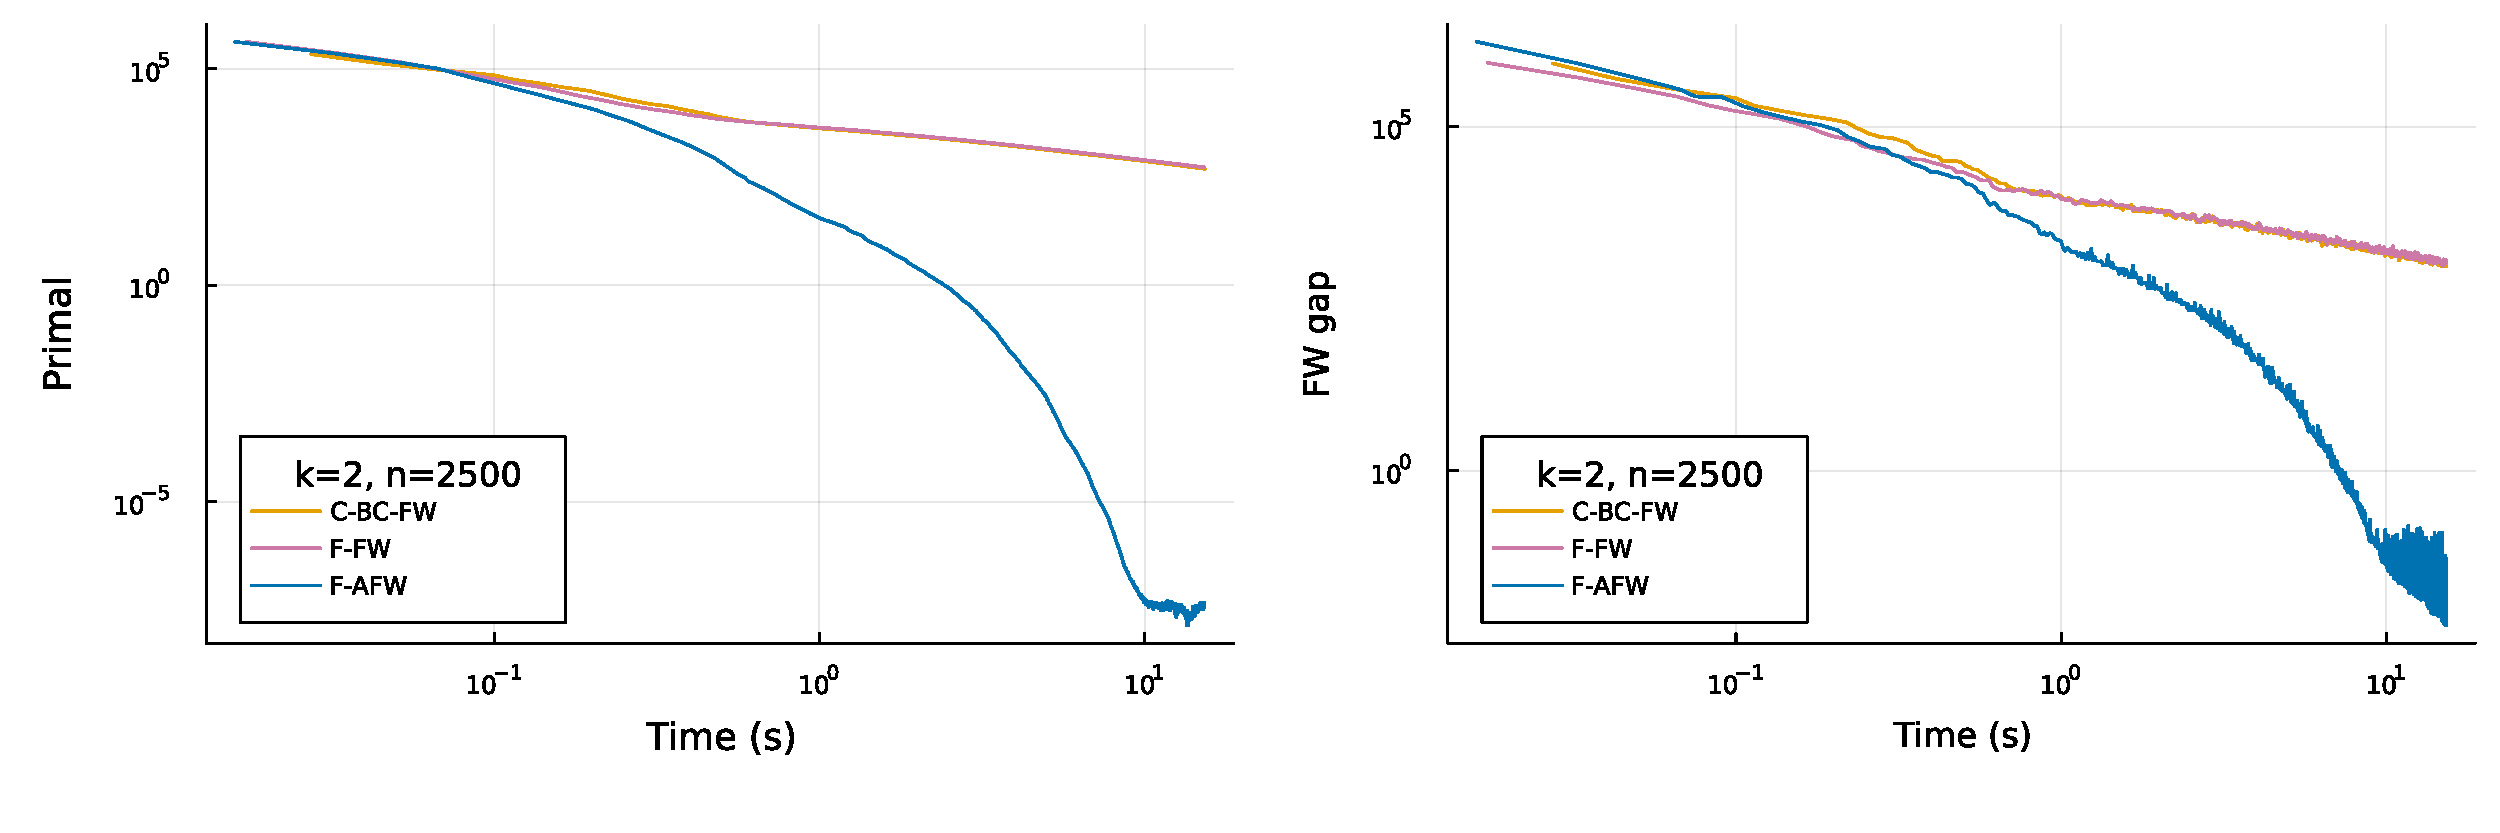
\includegraphics[width=\textwidth]{./figures/plot_ni_k2_n2500_i1000_s240389_cvxho_anc_t20250514_114746_fromlogs}
\caption{FW variants, run for up to $1\,000$ iterations on two non-intersecting point-cloud polytopes in $\R^{2\,500}$. }
\label{fig:k2n2500_pc_ni}
\end{figure}
%

\begin{figure}[!t]
\centering
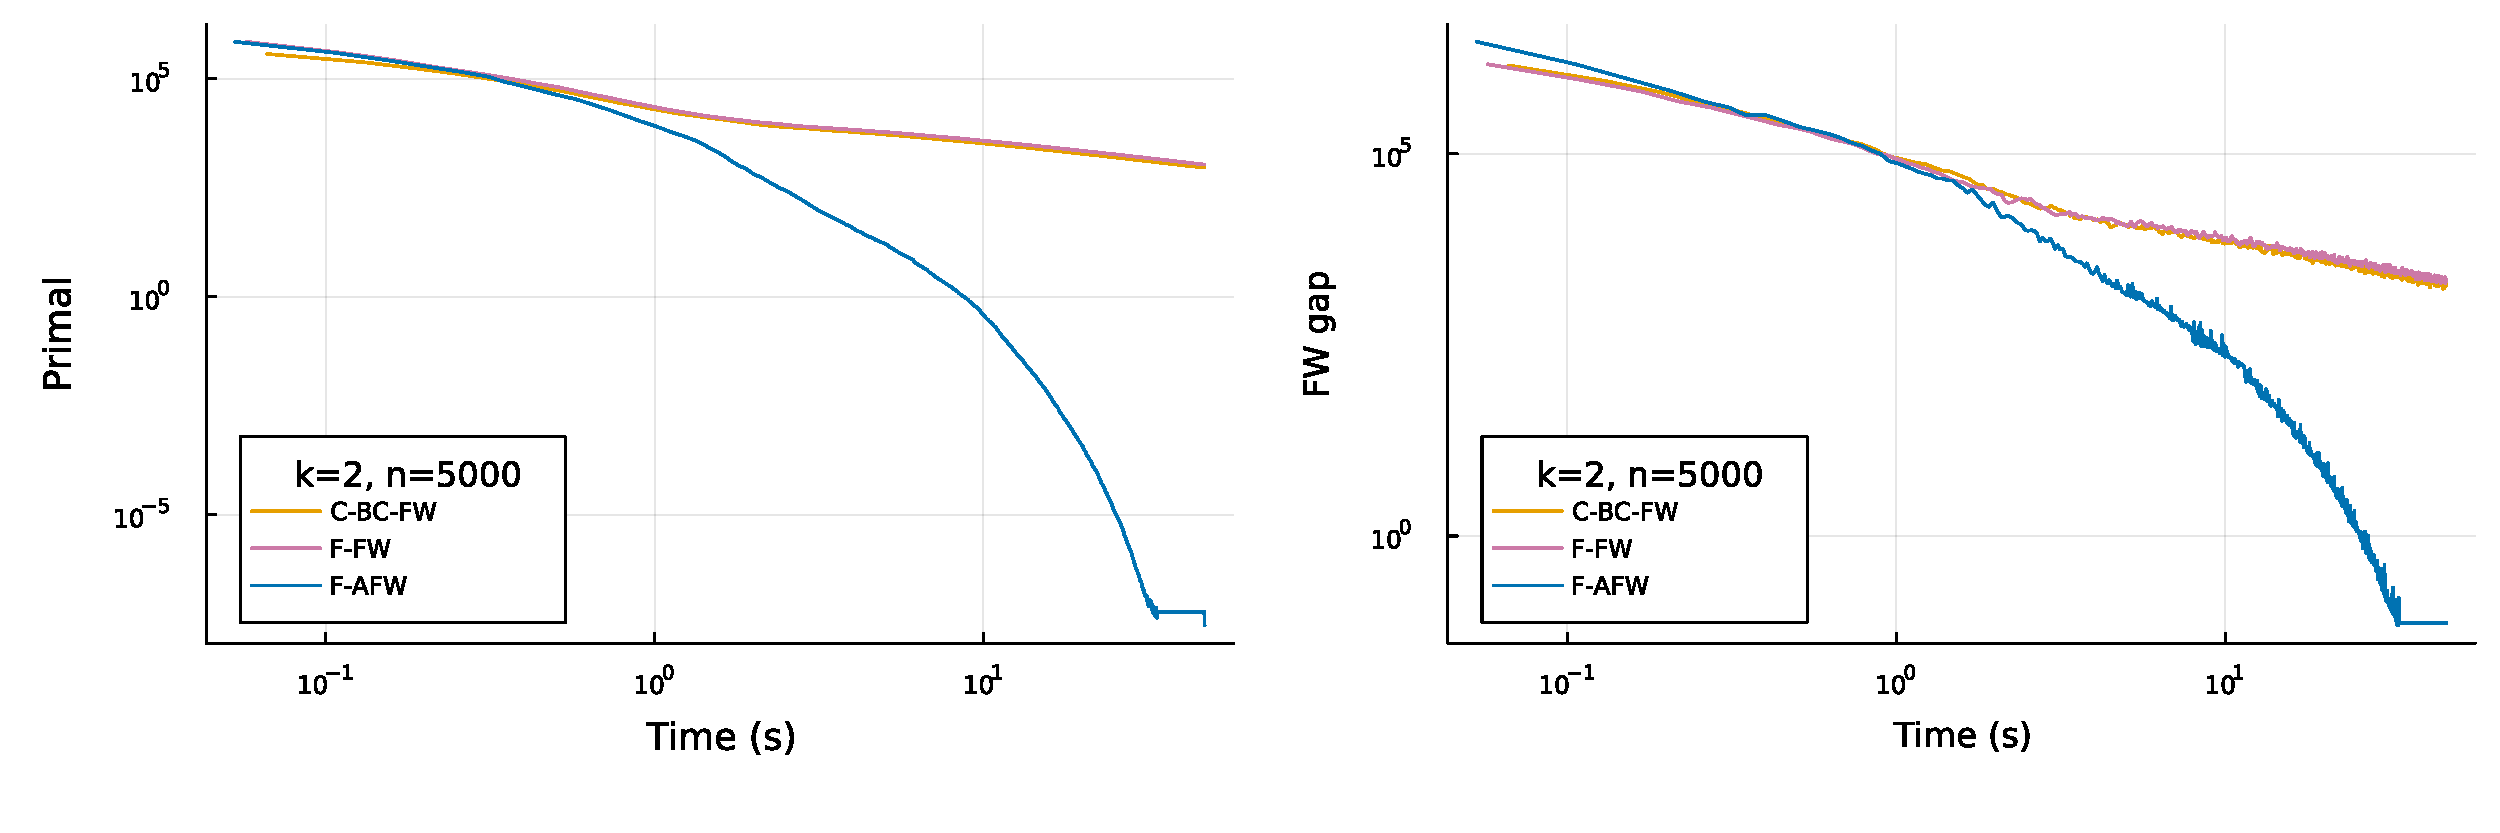
\includegraphics[width=\textwidth]{./figures/plot_ni_k2_n5000_i1000_s240389_cvxho_anc_t20250514_113038_fromlogs}
\caption{\FW{} variants, run for up to $1\,000$ iterations on two non-intersecting point-cloud polytopes in $\R^{5\,000}$. }
\label{fig:k2n5000_pc_ni}
\end{figure}
%

\begin{figure}[!t]
\centering
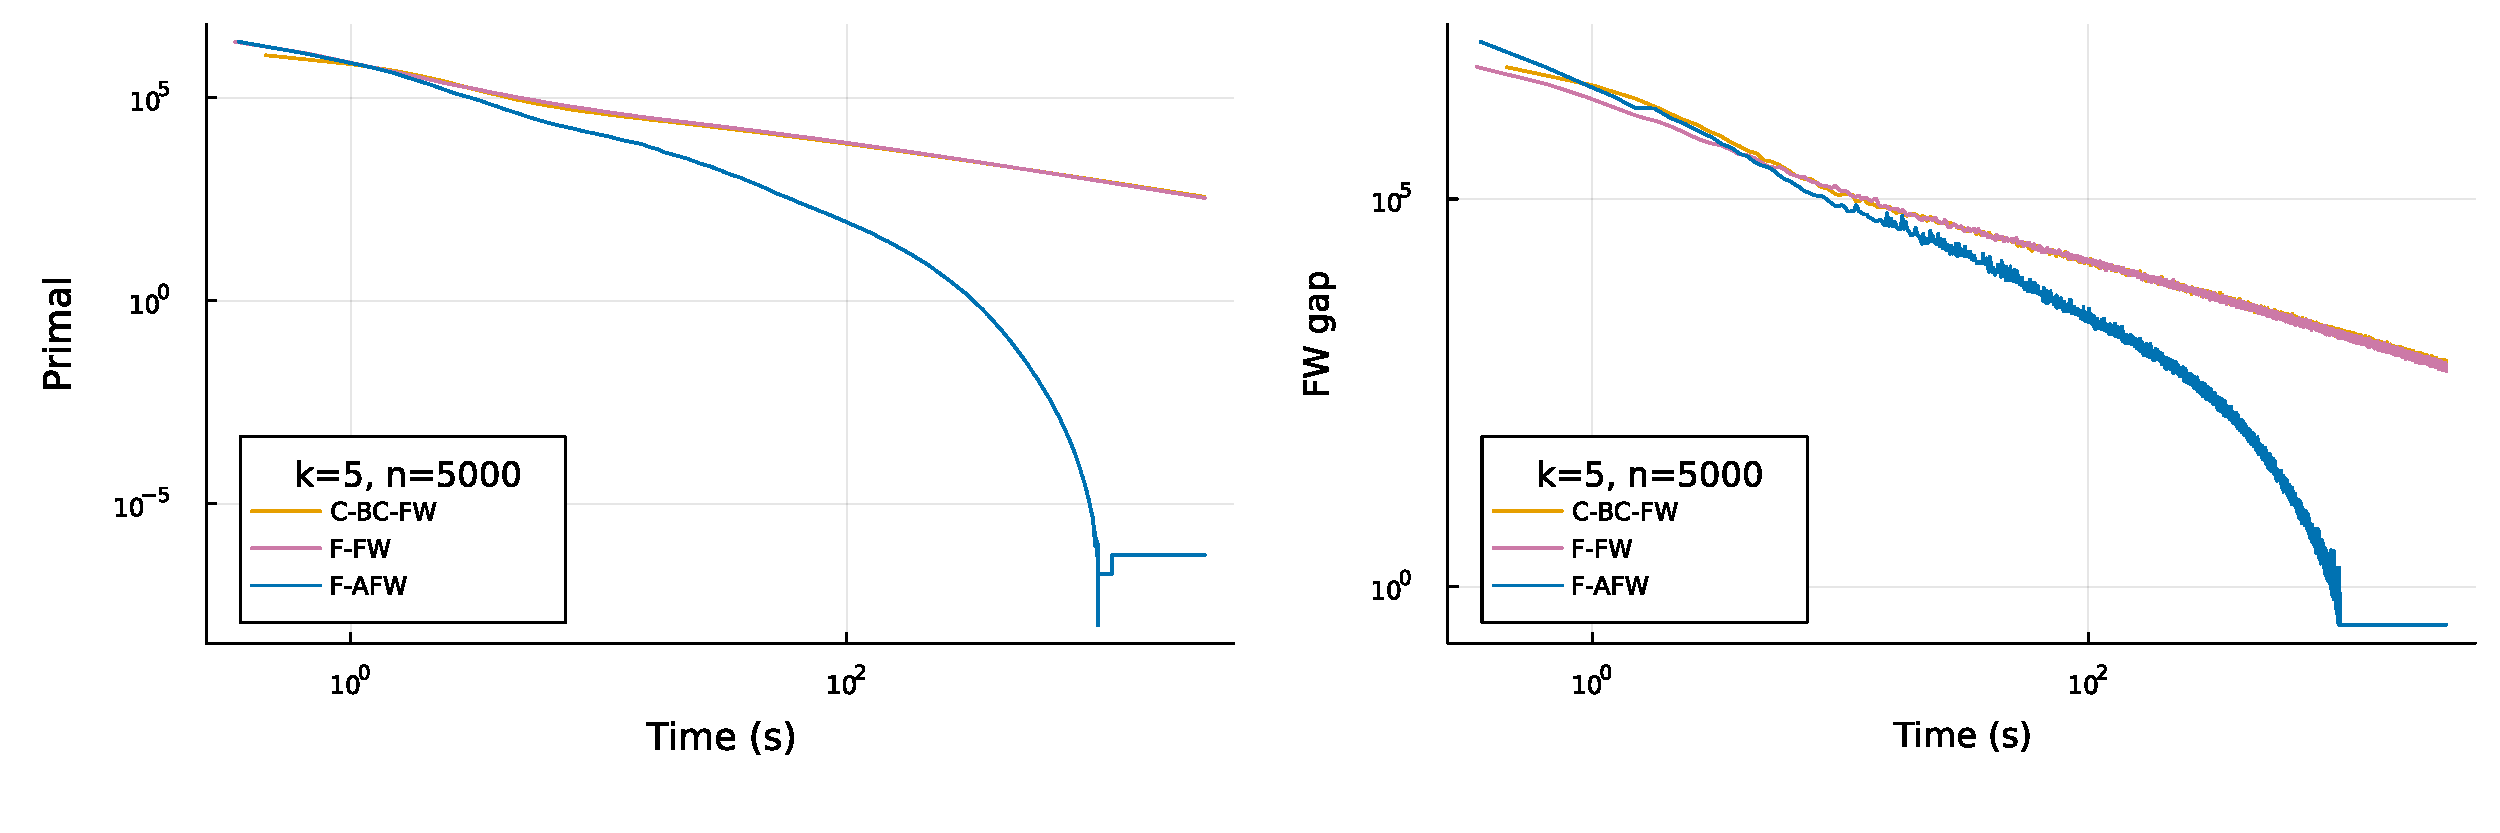
\includegraphics[width=\textwidth]{./figures/plot_ni_k5_n5000_npub25000_unif_i10000_s240389_cvxho-mat_a-p1_p2_segment-0.5_ref-vertex_t20260327_024217}
\caption{FW variants, run for up to $10\,000$ iterations on five non-intersecting point-cloud polytopes in $\R^{5\,000}$. For each polytope, we draw the number of points uniformly at random in $[n, 5n]$.}
\label{fig:k5n5000_pc_ni}
\end{figure}

%
\begin{figure}[!t]
\centering
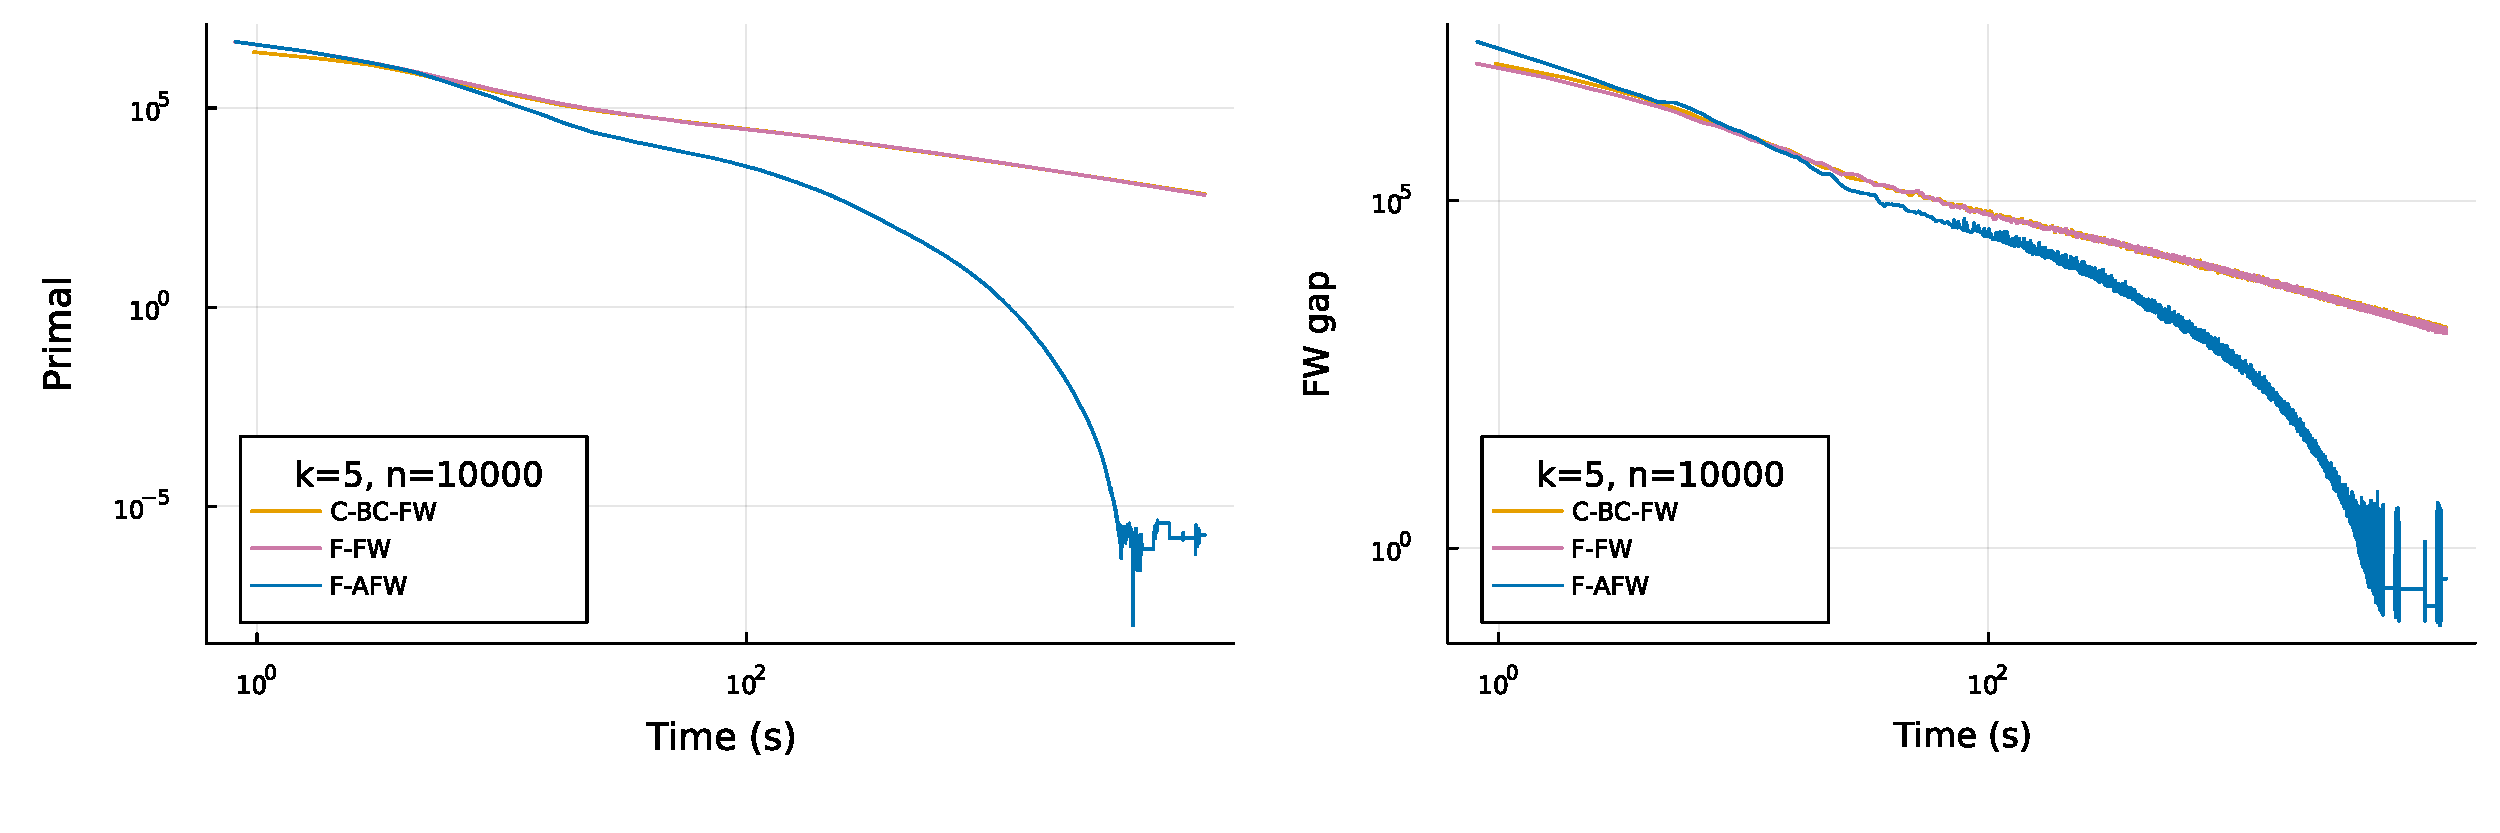
\includegraphics[width=\textwidth]{./figures/plot_ni_k5_n10000_npub50000_unif_i10000_s344_cvxho-mat_a-p1_p2_segment-0.5_ref-vertex_t20260327_064429}
\caption{FW variants, run for up to $10\,000$ iterations on five non-intersecting point-cloud polytopes in $\R^{10\,000}$. For each polytope, we draw the number of points uniformly at random in $[n, 5n]$.}
\label{fig:k5n10000_pc_ni}
\end{figure}

%
\begin{figure}[!t]
\centering
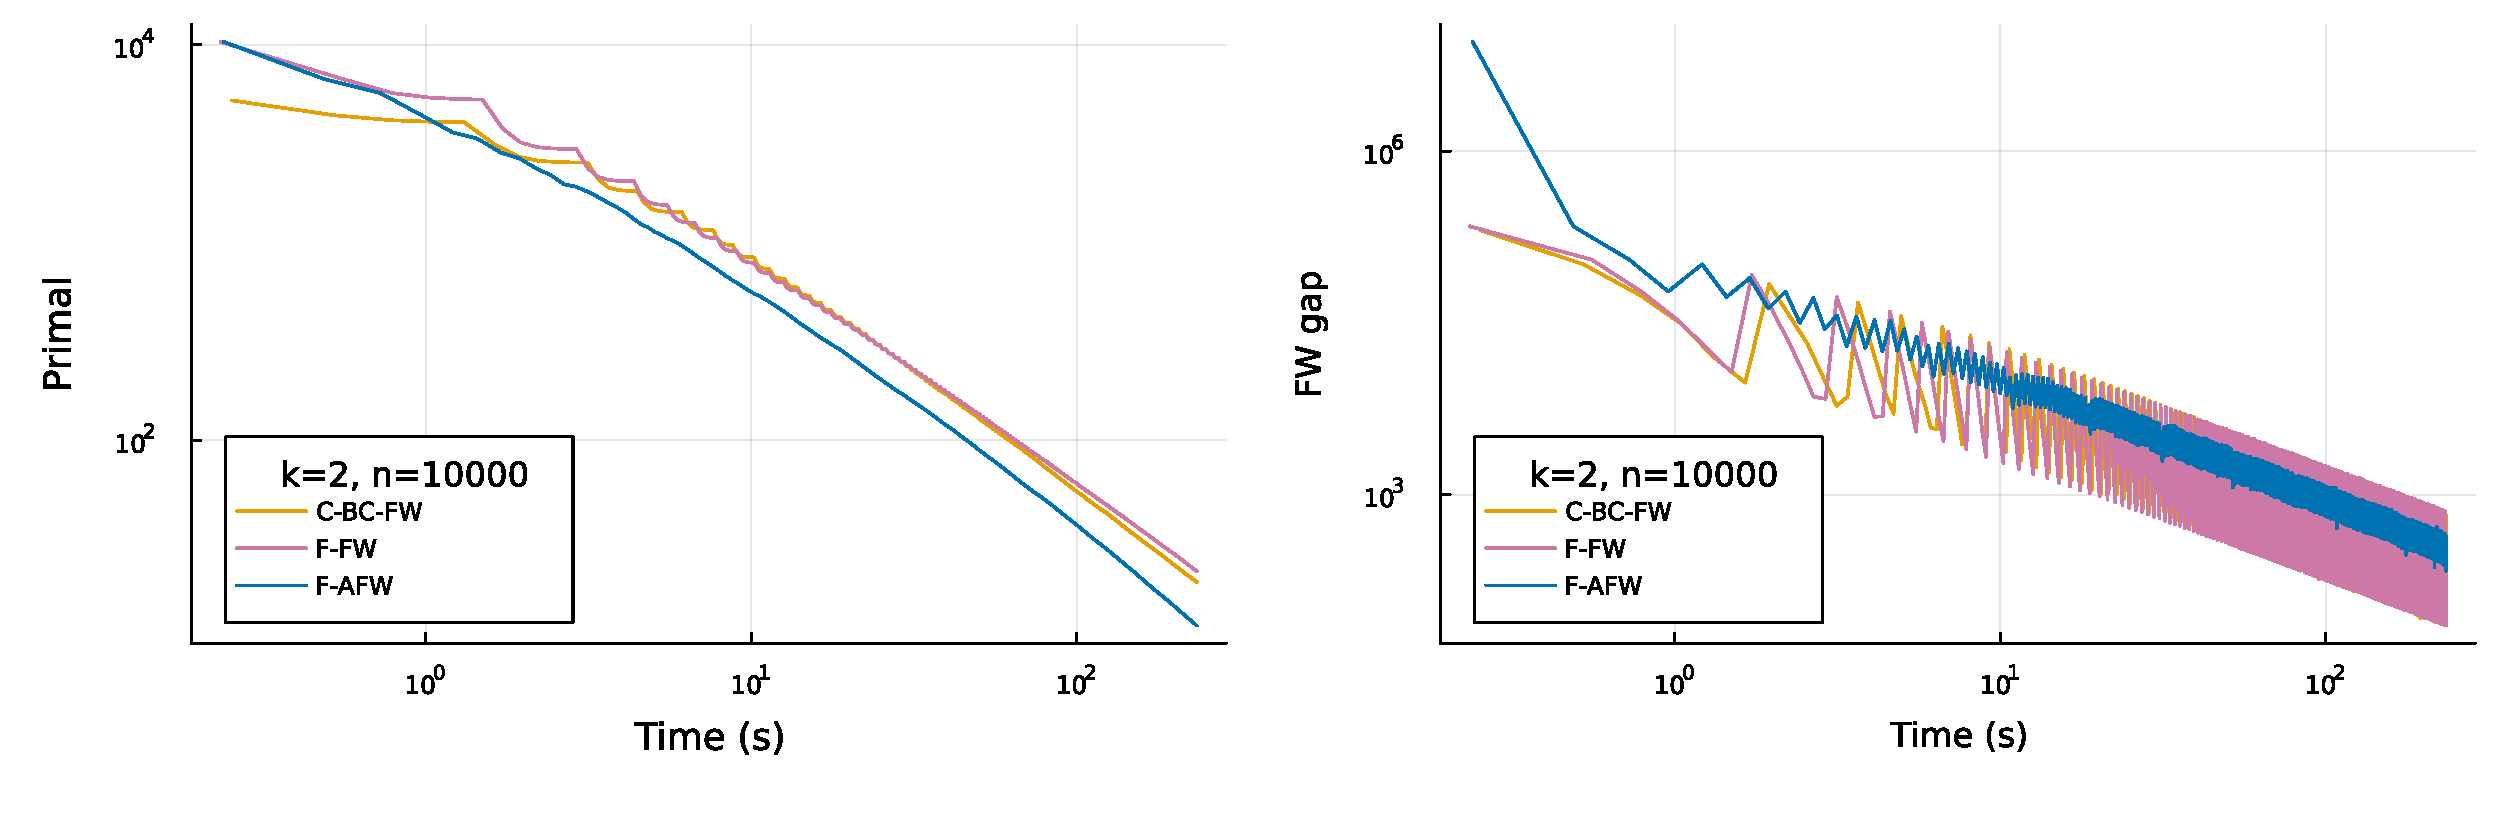
\includegraphics[width=\textwidth]{./figures/plot_i_k2_n10000_i1000_s240389_cvxho_anc_t20250511_123700_fromlogs}
\caption{FW variants, run for up to $1\,000$ iterations on two intersecting point-cloud polytopes in $\R^{10\,000}$. }
\label{fig:k2n10000_pc_i}
\end{figure}

%
\begin{figure}[!t]
\centering
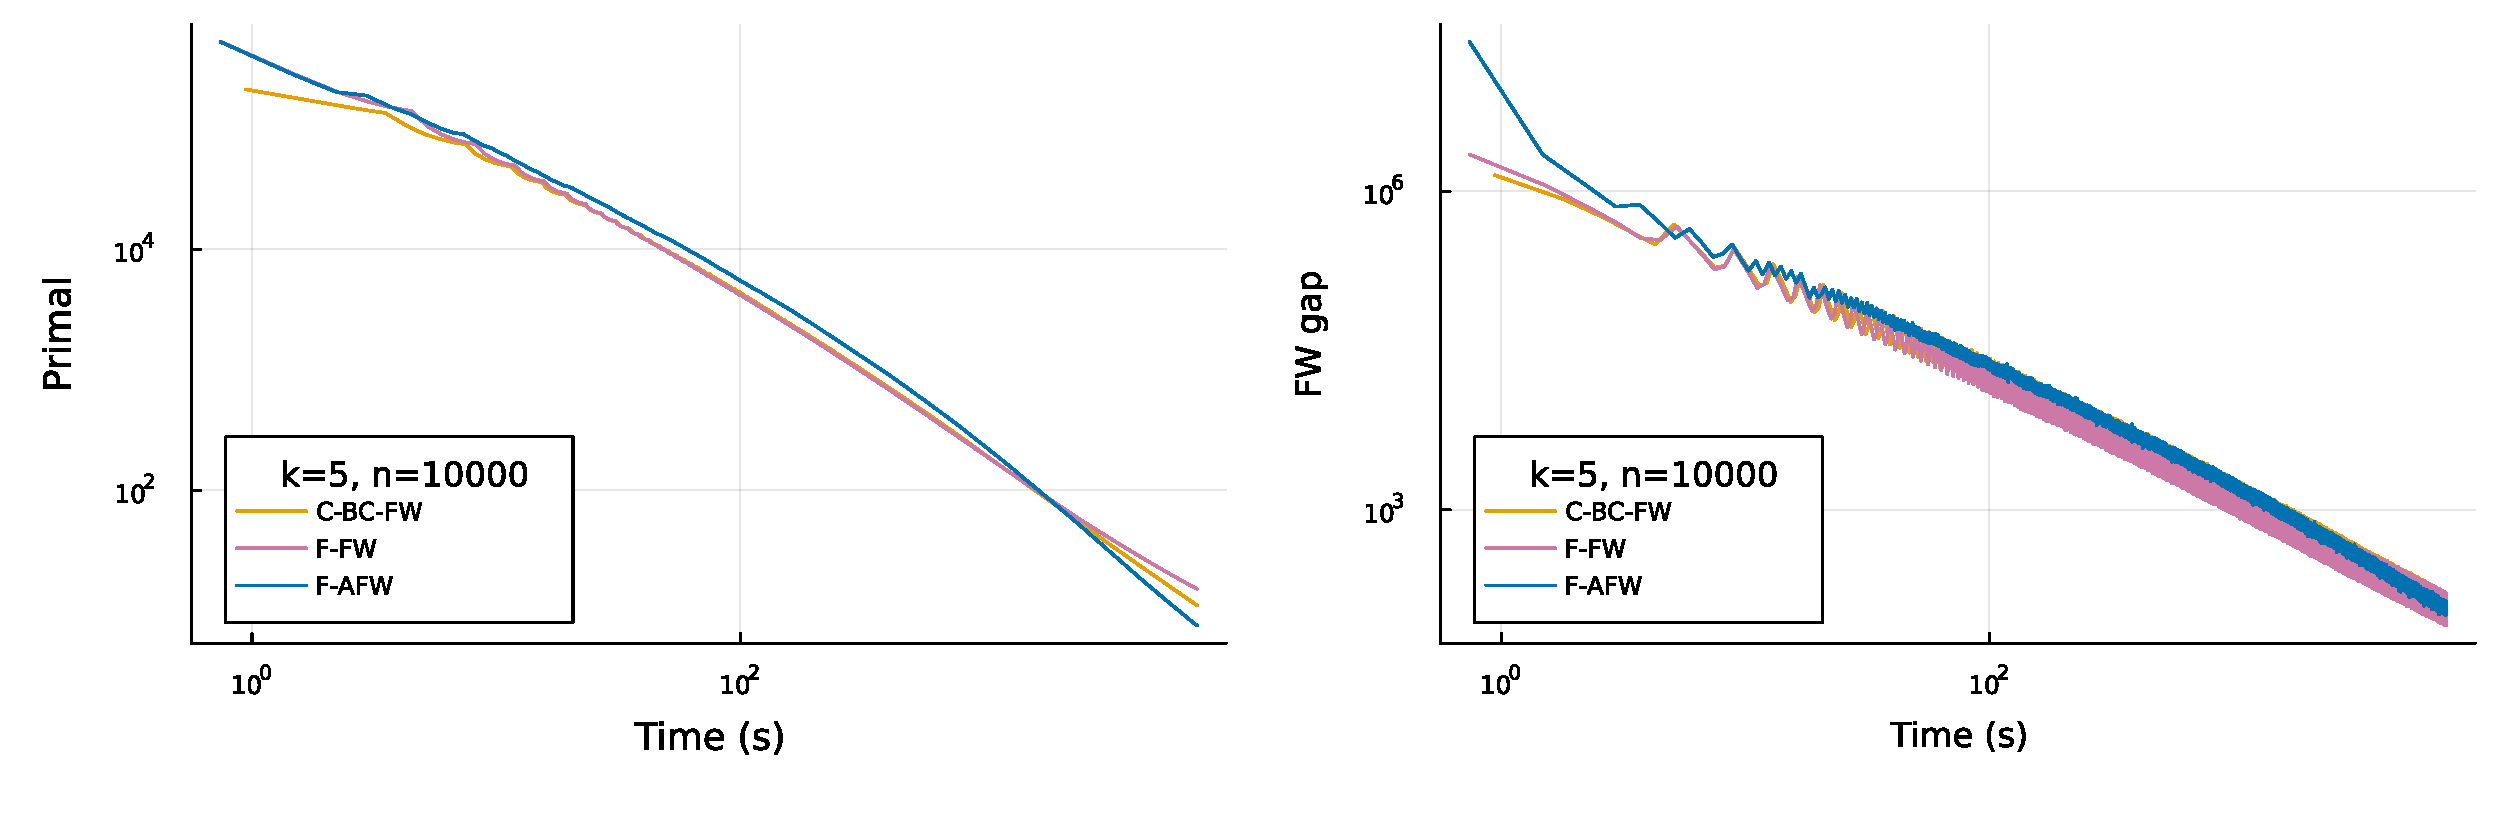
\includegraphics[width=\textwidth]{./figures/plot_i_k5_n10000_npub50000_unif_i10000_s344_cvxho-mat_a-p1_p2_segment-0.5_ref-vertex_t20260327_064429}
\caption{FW variants, run for up to $10\,000$ iterations on the five intersecting point-cloud polytopes from \cref{fig:k5n10000_pc_ni}, here translated to intersect. For each polytope, we draw the number of points uniformly at random in $[n, 5n]$.}
\label{fig:k5n10000_pc_i}
\end{figure}


\gabaistats{
We also include new vertex-facet experiments in \cref{fig:k2n10000_vf_ni,fig:k2n20000_vf_ni,fig:k2n20000_vf_i}.
\cref{fig:k2n10000_vf_ni} complements the $n=10\,000$ intersecting vertex-facet instance from the main text by showing the corresponding non-intersecting construction.
\cref{fig:k2n20000_vf_ni,fig:k2n20000_vf_i} further extend this family to dimension $20\,000$, in both the non-intersecting and intersecting settings.
Across these additional vertex-facet plots, \AFW{} again exhibits the clearest linear regime and maintains a marked advantage over the FW-based baselines, which is consistent with the sharper local geometry induced by the vertex-facet construction.
}

\begin{figure}[!t]
\centering
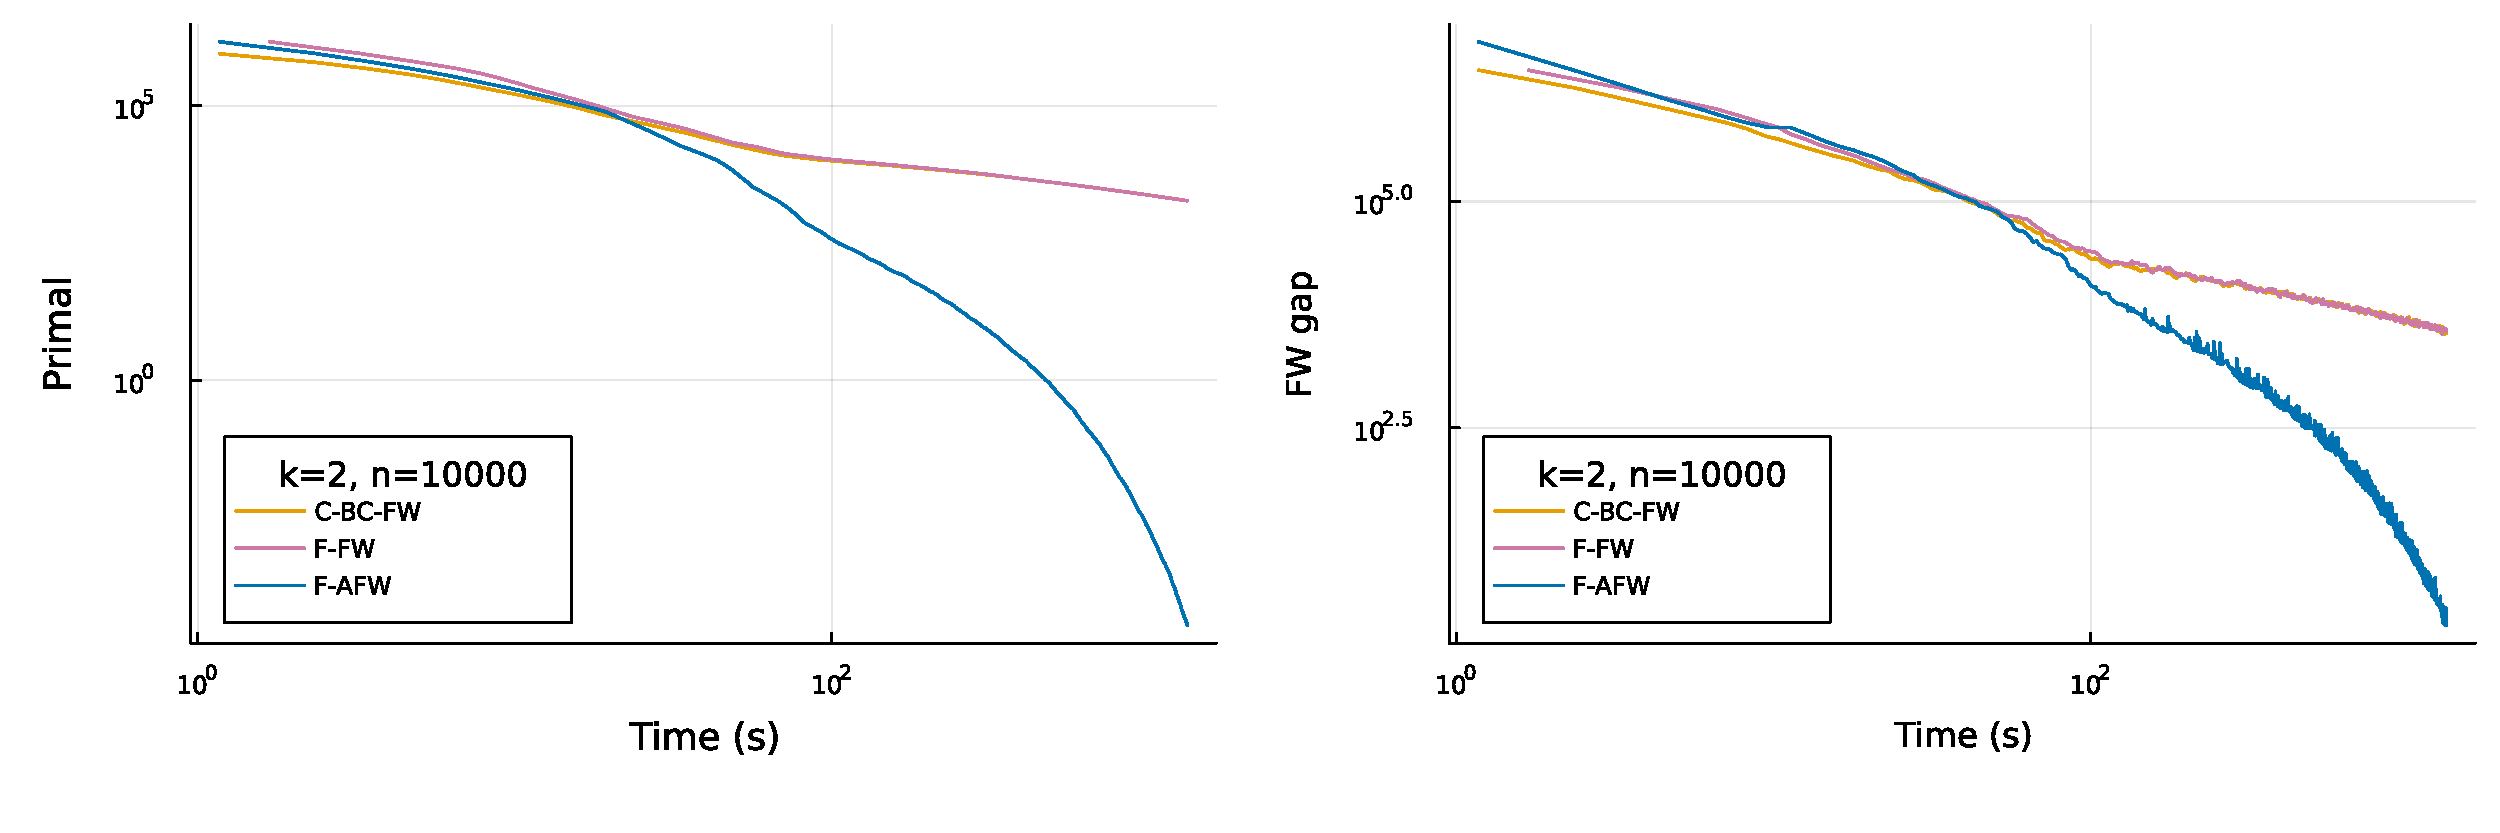
\includegraphics[width=\textwidth]{./figures/plot_ni_k2_n10000_i1000_s240389_cvxho_vert_t20250513_175132_fromlogs_100000vertices}
\caption{FW variants, run for up to $1\,000$ iterations on two non‑intersecting point-cloud polytopes in $\R^{10\,000}$, generated as the convex hull of $100\,000$ vertices.}
\label{fig:k2n10000_100000vertices_pc_ni}
\end{figure}

\begin{figure}[!t]
\centering
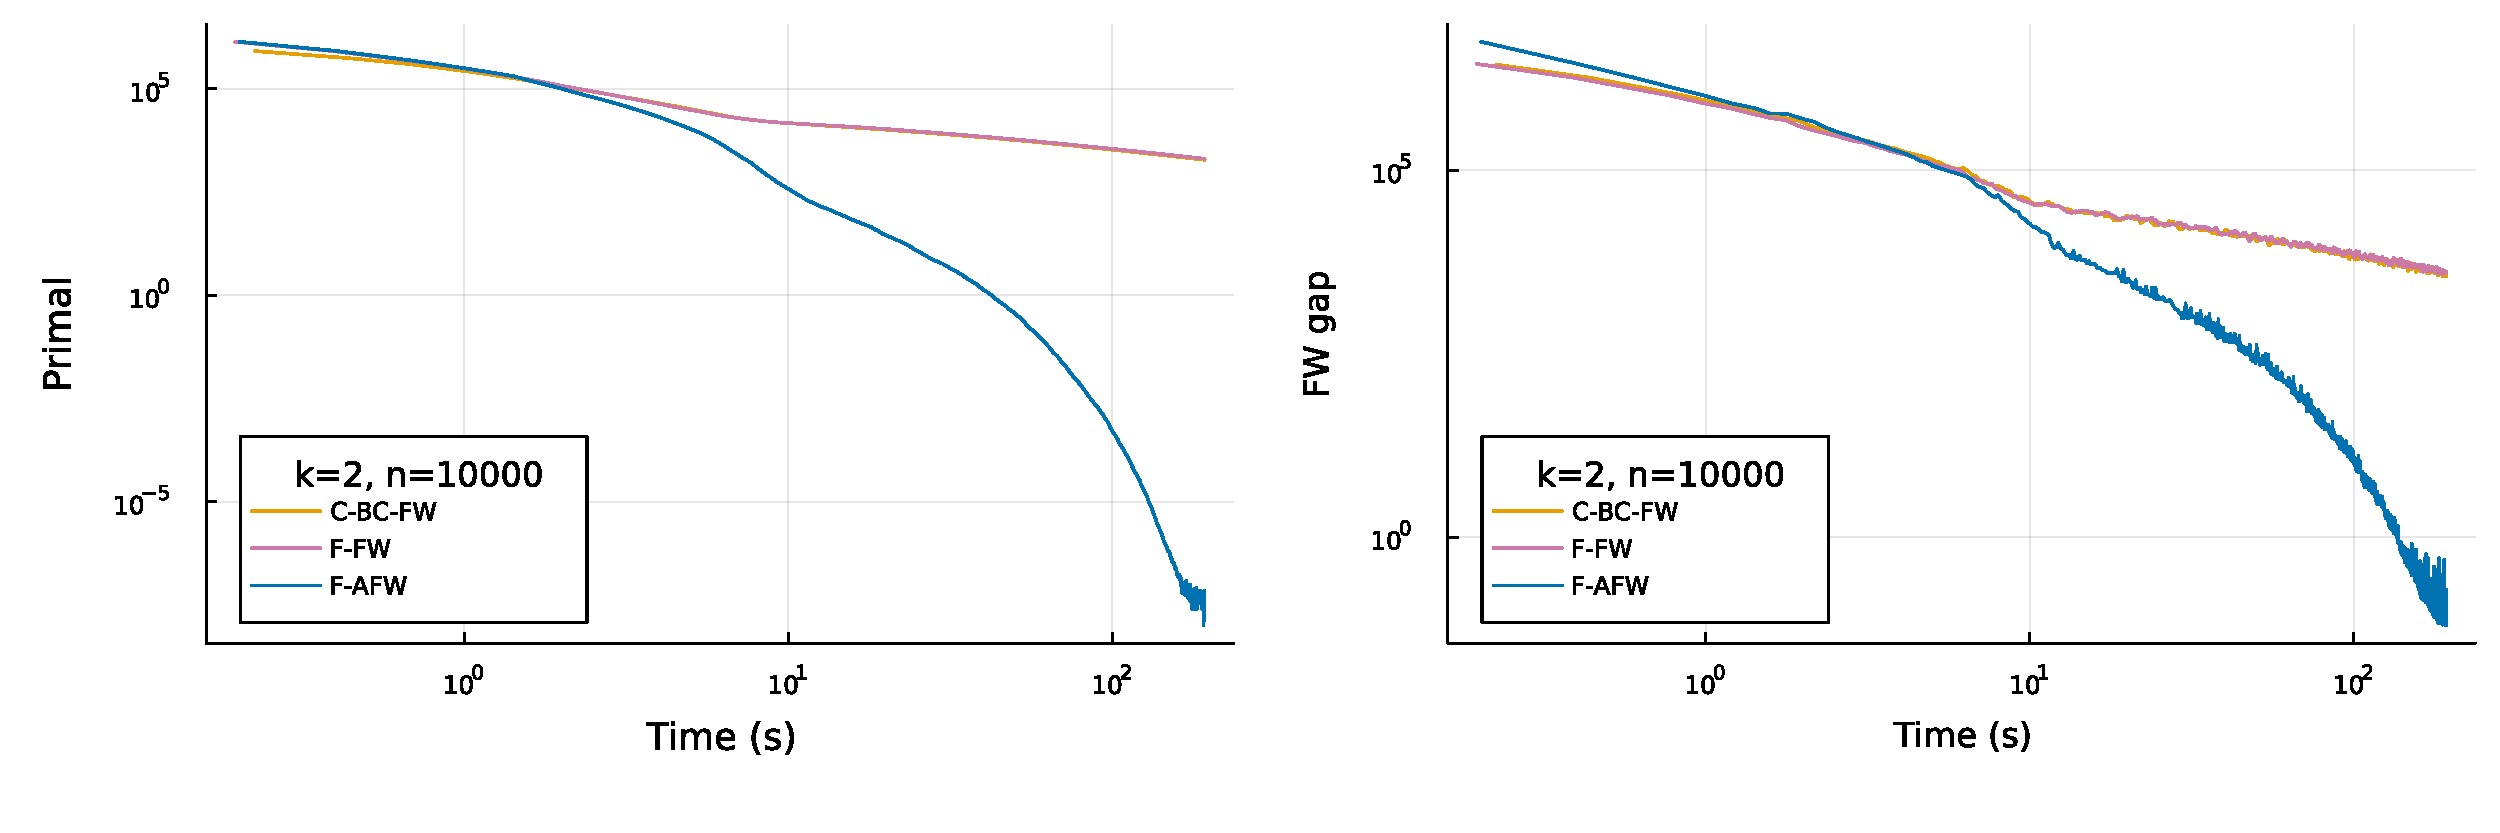
\includegraphics[width=\textwidth]{./figures/plot_ni_k2_n10000_i1000_s6_cvxho_anc_t20250515_121134_fromlogs}
\caption{FW variants, run for up to $1\,000$ iterations on two non‑intersecting point-cloud polytopes in $\R^{10\,000}$, generated as the convex hull of $15\,000$ vertices.}
\label{fig:k2n10000_15000vertices_pc_ni}
\end{figure}


\begin{figure}[!t]
\centering
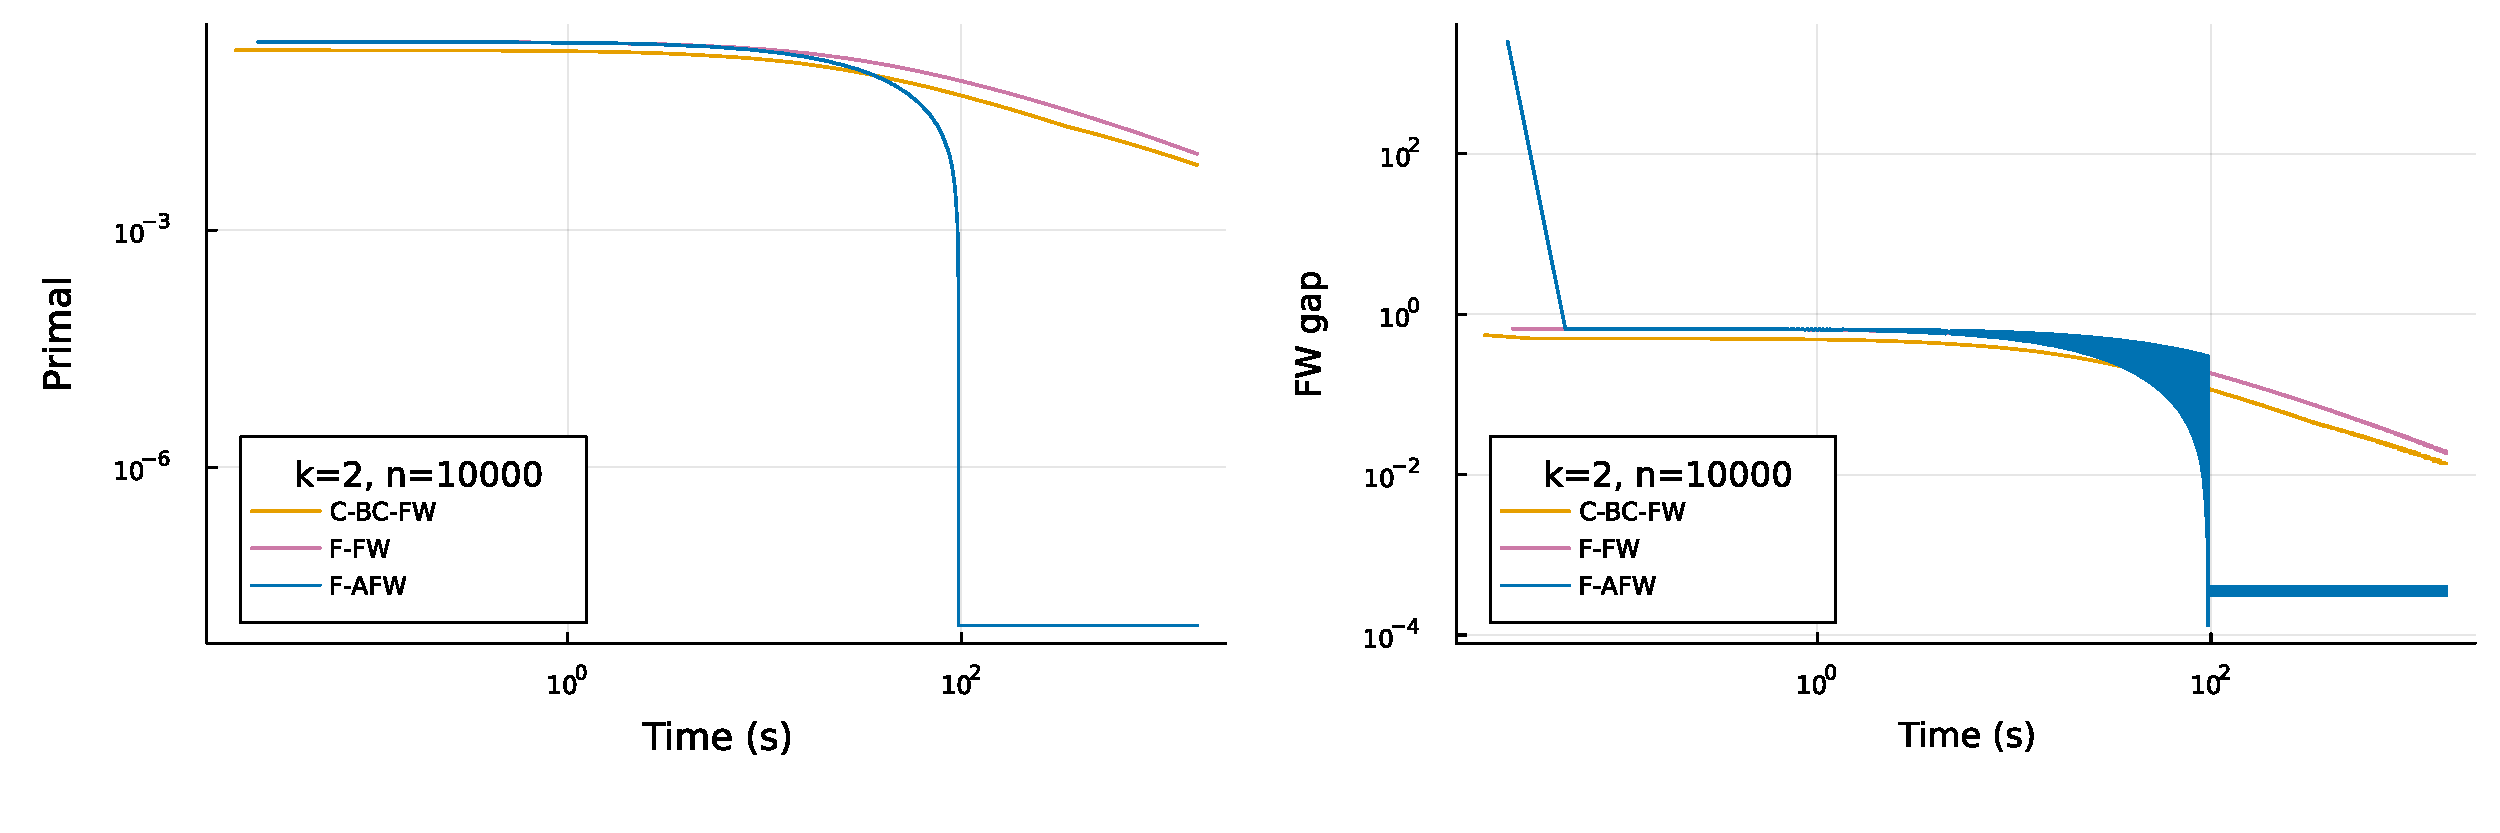
\includegraphics[width=\textwidth]{./figures/plot_ni_vf_k2_n10000_i80000_s42_a0p1_b0p3_d0p45_tp-mid_sep-0p5_t20260324_022349}
\caption{FW variants, run for up to $80\,000$ iterations on the two vertex-facet polytopes from \cref{fig:k2n10000_vf_i}, not intersecting here.}
\label{fig:k2n10000_vf_ni}
\end{figure}


\begin{figure}[!t]
\centering
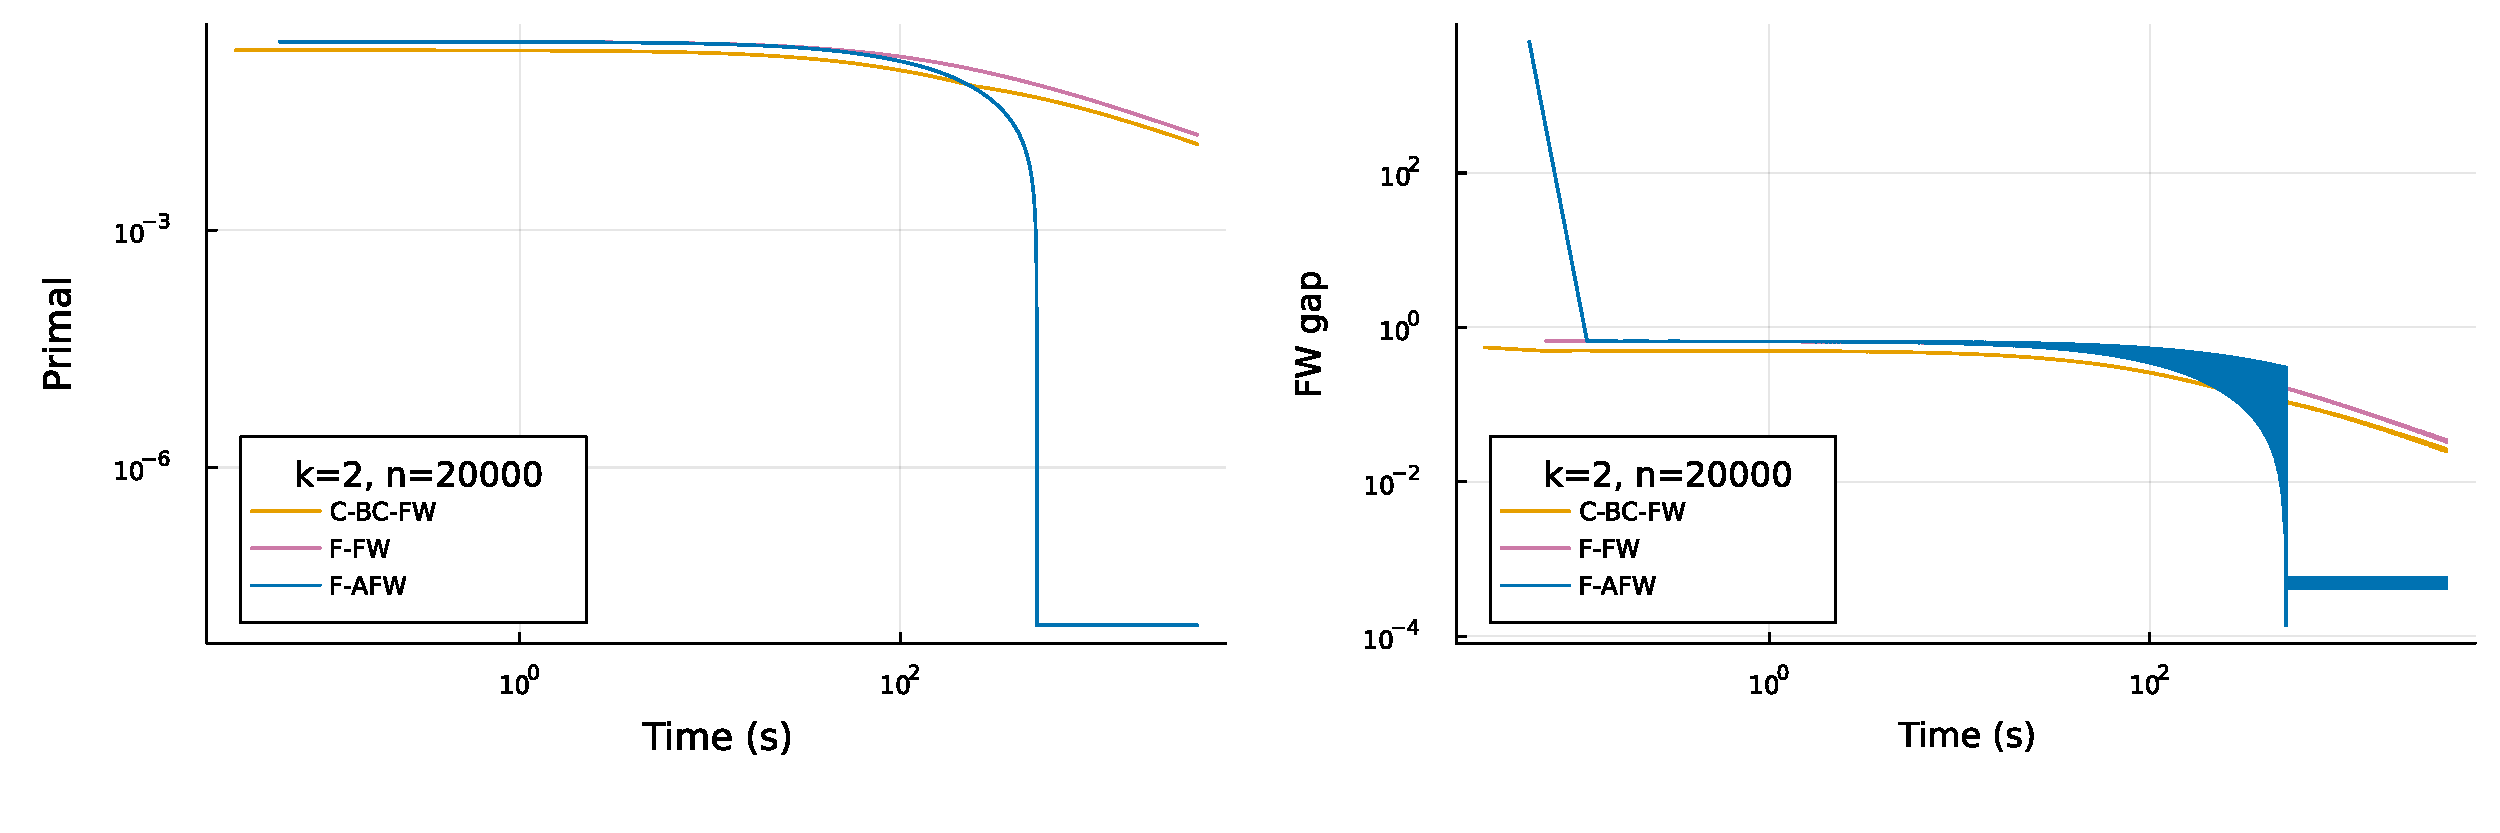
\includegraphics[width=\textwidth]{./figures/plot_ni_vf_k2_n20000_i80000_s42_a0p1_b0p3_d0p45_tp-mid_sep-0p5_t20260328_030828}
\caption{FW variants, run for up to $80\,000$ iterations on two non-intersecting vertex-facet polytopes in $\R^{20\,000}$.}
\label{fig:k2n20000_vf_ni}
\end{figure}

\begin{figure}[!t]
\centering
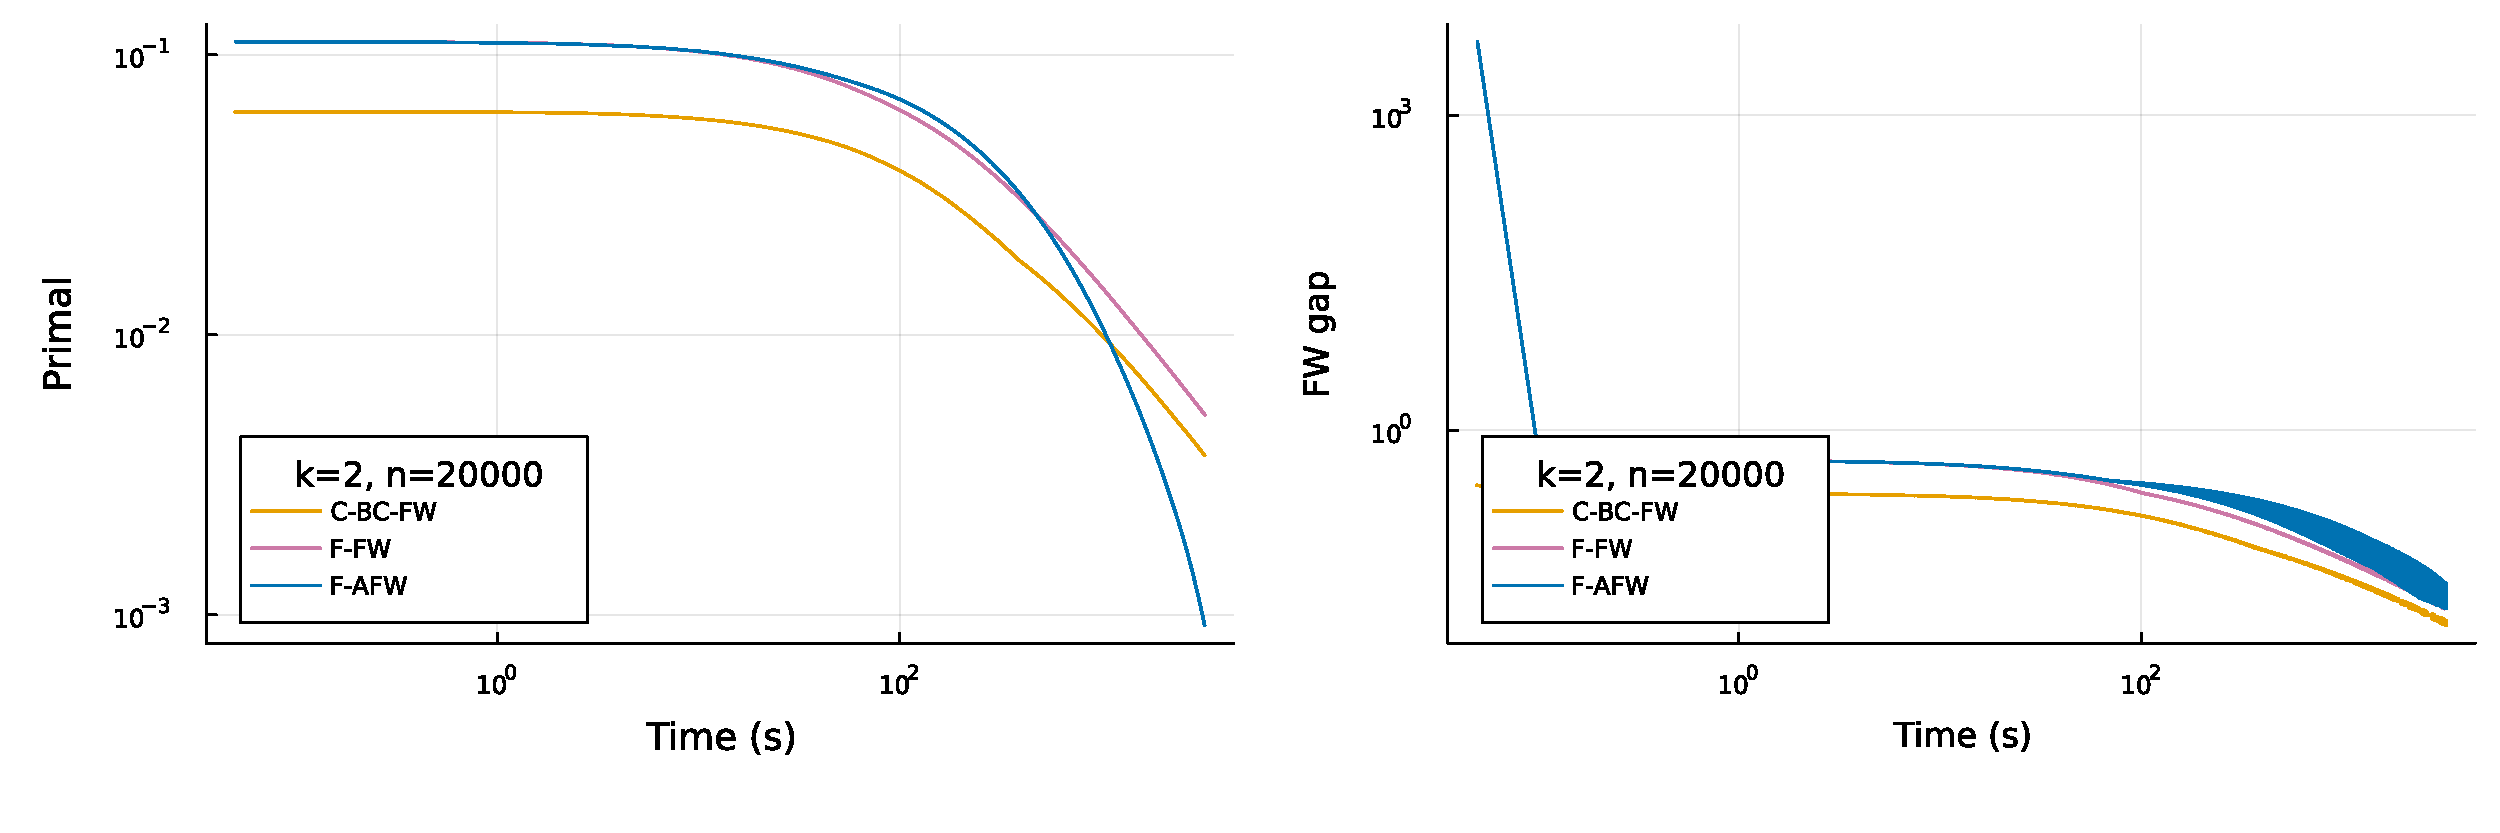
\includegraphics[width=\textwidth]{./figures/plot_i_vf_k2_n20000_i80000_s42_a0p1_b0p3_d0p45_tp-mid_sep-0p5_t20260328_030828}
\caption{FW variants, run for up to $80\,000$ iterations on the two vertex-facet polytopes from \cref{fig:k2n20000_vf_ni}, here translated to intersect.}
\label{fig:k2n20000_vf_i}
\end{figure}

% --------------------


\end{document}
